\documentclass{article}

  % packages
    % basic stuff for rendering math
    \usepackage[letterpaper, top=1in, bottom=1in, left=1in, right=1in]{geometry}
    \usepackage{extarrows, esvect, esint, pgfplots}
    \usepackage[utf8]{inputenc}
    \usepackage[english]{babel}
    \usepackage{amsmath} 
    \usepackage{amssymb}

    % extra math symbols and utilities
    \usepackage{mathtools}        % for extra stuff like \coloneqq
    \usepackage{mathrsfs}         % for extra stuff like \mathsrc{}
    \usepackage{centernot}        % for the centernot arrow 
    \usepackage{bm}               % for better boldsymbol/mathbf 
    \usepackage{enumitem}         % better control over enumerate, itemize
    \usepackage{hyperref}         % for hypertext linking
    \usepackage{xr-hyper}
    \usepackage{fancyvrb}          % for better verbatim environments
    \usepackage{newverbs}         % for texttt{}
    \usepackage{xcolor}           % for colored text 
    \usepackage{listings}         % to include code
    \usepackage{lstautogobble}    % helper package for code
    \usepackage{parcolumns}       % for side by side columns for two column code
    

    % page layout
    \usepackage{fancyhdr}         % for headers and footers 
    \usepackage{lastpage}         % to include last page number in footer 
    \usepackage{parskip}          % for no indentation and space between paragraphs    
    \usepackage[T1]{fontenc}      % to include \textbackslash
    \usepackage{footnote}
    \usepackage{etoolbox}

    % for custom environments
    \usepackage{tcolorbox}        % for better colored boxes in custom environments
    \tcbuselibrary{breakable}     % to allow tcolorboxes to break across pages

    % figures
    \usepackage{pgfplots}
    \pgfplotsset{compat=1.18}
    \usepackage{float}            % for [H] figure placement
    \usepackage{tikz}
    \usepackage{tikz-cd}
    \usepackage{circuitikz}
    \usetikzlibrary{arrows}
    \usetikzlibrary{positioning}
    \usetikzlibrary{calc}
    \usetikzlibrary{patterns}
    \usepackage{graphicx}
    \usepackage{algorithm, algpseudocode}
    \usepackage{caption} 
    \usepackage{subcaption}
    \captionsetup{font=small}

    % for tabular stuff 
    \usepackage{dcolumn}

    \usepackage[nottoc]{tocbibind}
    \pdfsuppresswarningpagegroup=1
    \hfuzz=5.002pt                % ignore overfull hbox badness warnings below this limit

  % New and replaced operators
    \DeclareMathOperator{\Tr}{Tr}
    \DeclareMathOperator{\Sym}{Sym}
    \DeclareMathOperator{\Span}{span}
    \DeclareMathOperator{\im}{Im}
    \DeclareMathOperator{\Div}{div}
    \DeclareMathOperator{\curl}{curl}
    \DeclareMathOperator{\GL}{GL}
    \DeclareMathOperator{\SL}{SL}
    \DeclareMathOperator{\GA}{GA}
    \DeclareMathOperator{\std}{std}
    \DeclareMathOperator{\Cov}{Cov}
    \DeclareMathOperator{\Var}{Var}
    \DeclareMathOperator{\Corr}{Corr}
    \DeclareMathOperator{\Int}{Int}
    \DeclareMathOperator{\Id}{Id}
    \DeclareMathOperator{\Lie}{Lie}
    \DeclareMathOperator{\Hom}{Hom}
    \DeclareMathOperator{\Alt}{Alt}
    \DeclareMathOperator{\rank}{rank}
    \DeclareMathOperator{\conv}{conv}
    \DeclareMathOperator{\aff}{aff}
    \DeclareMathOperator{\arccot}{arccot}
    \DeclareMathOperator*{\argmin}{\arg\!\min}
    \DeclareMathOperator*{\argmax}{\arg\!\max}
    \newcommand{\ket}[1]{\ensuremath{\left|#1\right\rangle}}
    \newcommand{\bra}[1]{\ensuremath{\left\langle#1\right|}}
    \newcommand{\braket}[2]{\langle #1 | #2 \rangle}
    \newcommand{\qed}{\hfill$\blacksquare$}     % I like QED squares to be black

  % Custom Environments
    \tcbset{
      colframe = black,
      colback  = white,
      coltitle = black,
      colbacktitle = black!10,
      breakable, 
      arc=0mm,
      boxrule=1pt,
      left=8pt,
      right=8pt,
      top=6pt,
      bottom=6pt,
      before skip=12pt,
      after skip=12pt,
      bottomrule at break=-1pt,
      toprule at break=-1pt,
      fonttitle=\bfseries,
    }
    \newtcolorbox[auto counter, number within=section]{question}[1][]
    {
      title = \textbf{Question \thetcbcounter ~(#1)}
    }
    \newtcolorbox[auto counter, number within=section]{exercise}[1][]
    {
      title = \textbf{Exercise \thetcbcounter ~(#1)}
    }
    \newtcolorbox[auto counter, number within=section]{solution}[1][]
    {
      title = \textbf{Solution \thetcbcounter}
    }
    \newtcolorbox[auto counter, number within=section]{lemma}[1][]
    {
      title = \textbf{Lemma \thetcbcounter ~(#1)},
    }
    \newtcolorbox[auto counter, number within=section]{theorem}[1][]
    {
      title = \textbf{Theorem \thetcbcounter ~(#1)},
    } 
    \newtcolorbox[auto counter, number within=section]{corollary}[1][]
    {
      title = \textbf{Corollary \thetcbcounter ~(#1)},
    } 
    \newtcolorbox[auto counter, number within=section]{proof}[1][]
    {
      before skip = -7pt,
      before upper = \textit{Proof. },
    } 
    \newtcolorbox[auto counter, number within=section]{definition}[1][]
    {
      title = \textbf{Definition \thetcbcounter ~(#1)}
    }
    \newtcolorbox[auto counter, number within=section]{example}[1][]
    {
      title = \textbf{Example \thetcbcounter ~(#1)}
    } 
    \newtcolorbox[auto counter, number within=section]{code}[1][]
    {
      title = \textbf{Code \thetcbcounter ~(#1)}
    } 

    \definecolor{dkgreen}{rgb}{0,0.6,0}
    \definecolor{gray}{rgb}{0.5,0.5,0.5}
    \definecolor{mauve}{rgb}{0.58,0,0.82}
    \definecolor{lightgray}{gray}{0.93}

    % default options for listings (for code)
    \lstset{
      autogobble,
      frame=ltbr,
      language=C,                           % the language of the code
      aboveskip=3mm,
      belowskip=3mm,
      showstringspaces=false,
      columns=fullflexible,
      keepspaces=true,
      basicstyle={\small\ttfamily},
      numbers=left,
      firstnumber=1,                        % start line number at 1
      numberstyle=\tiny\color{gray},
      keywordstyle=\color{blue},
      commentstyle=\color{dkgreen},
      stringstyle=\color{mauve},
      backgroundcolor=\color{lightgray}, 
      breaklines=true,                      % break lines
      breakatwhitespace=true,
      tabsize=3, 
      xleftmargin=2em, 
      framexleftmargin=1.5em, 
      stepnumber=1
    }

  % Page style
    \pagestyle{fancy}
    \fancyhead[L]{Multivariate Real Analysis}
    \fancyhead[C]{Muchang Bahng}
    \fancyhead[R]{Spring 2025} 
    \fancyfoot[C]{\thepage / \pageref{LastPage}}
    \renewcommand{\footrulewidth}{0.4pt}          % the footer line should be 0.4pt wide
    \renewcommand{\thispagestyle}[1]{}  % needed to include headers in title page

  % external documents
   \externaldocument[la-]{../Linear_Algebra/paper}[../Linear_Algebra/paper.pdf] 

\begin{document}

\title{Multivariate Real Analysis}
\author{Muchang Bahng}
\date{Spring 2025}

\maketitle
\tableofcontents
\pagebreak

Unlike my machine learning notes, which focuses mostly on the theoretical soundness of classical (e.g. pre-deep and interpretable) models, the theory of deep neural networks have not been developed as well yet. Furthermore, the recency of developments, especially in the post-2010s, results in a pretty nonlinear\footnote{No pun intended.} timeline that is difficult to categorize effectively. Before I give my motivation, the direct prerequisites for deep learning are basic knowledge of my notes in probability theory, machine learning, and real analysis. 

Therefore, after much thought, I think organizing my notes in chronological order would be best. It turned out that in the early days of deep learning, most researchers like Andrew Ng stated that he focused on supervised models,\footnote{He states this in his podcast with Lex Fridman.} and it wasn't until the 2010s that the development of unsupervised models burgeoned. 

\begin{enumerate}
  \item We start by introducing \textit{multilayered perceptrons} (MLPs), which build upon generalized linear models (GLMs) that we have went over in machine learning. This is pretty much the ``foundational'' model that we will build on. We then talk a about practical methodologies regarding training and control. 

  \item Then we introduce the other two architectures. The \textit{convolutional neural network} (CNN) gives us a scalable way to perform sparse matrix multiplication efficiently, by taking advantage of locality. Then in \textit{recurrent neural networks} (RNNs), we are not limited to a single $n$-dimensional vector input and are able to process a time series of inputs.  
    
  \item With these building blocks, we are able take and two neural networks together to create an encoder-decoder model. The two main applications of this was dimensionality reduction with \textit{autoencoders}, followed by \textit{seq2seq} for machine translation between sequences of words.  

  \item The practical success of autoencoders led to the development of not just density estimation models, but \textit{generative} ones that seek to sample from the learned distribution. These generative models were ``deep'' extensions of the classical linear factor models resulting in \textit{restricted Boltzmann machines (RBMs)} and \textit{variational autoencoders (VAEs)}, which attempted to explicitly model an approximation of the true data generating distribution. More specifically, RBMs were \textit{energy models} that borrowed ideas from physics to learn a distribution of the form $p_X (x) = \frac{1}{Z} e^{-f_\theta (x)}$. To sample from this, researchers already had access to the established Markov Chain Monte Carlo (MCMC) algorithms designed for this exact problem. As for VAEs, these were trained and sampled through \textit{variational inference} methods. 

  \item In 2014, a completely new architecture composed of 2 neural networks competing each other gave rise to \textit{generative adversarial networks} (GANs) which blew RBMs and VAEs away. A similar architecture followed with \textit{generative stochastic networks} (GSNs).

  \item In 2016, \textit{normalizing flow models}, which attempted to model a smooth function that transformed simple latent variables to the true data generating distribution, were invented by Google DeepMind and surpassed GANs. 

  \item In 2017, \textit{attention} took the world by storm, which had drastically improved machine translation in seq2seq, and the resulting \textit{self-attention} plus the \textit{transformer} architectures led to the success of OpenAI's ChatGPT. 
\end{enumerate} 

Again, I emphasize that the math in these notes are not very advanced. However, implementing these simple models and training algorithms from scratch is a challenge in itself. I will go through implementing everything from scratch as if we were building a mini-version of PyTorch as we learn new topics. My implementations can be found \href{https://github.com/mbahng/pyember}{here}. 

\section{Banach Spaces}  

  Note that both the domain and codomain of a function $f: \mathbb{R}^n \to \mathbb{R}^m$ are vector spaces. However, Euclidean spaces have a lot of structure on them, and it is nice to identify the essential properties we need from these sets. It is essential that we work in vector spaces because when we define a derivative, we usually see some form that looks like 
  \begin{equation}
    \frac{f(x + h) - f(x)}{h}
  \end{equation} 
  Note the operations used here. First, we want a notion of addition in the domain ($x + h$) and the codomain $f(x + h) - f(x)$, along with some scalar multiplication when we multiply by $1/h$. A vector space precisely supports these operations and therefore is a natural choice. It is immediate that to define convergence, we definitely need a topology. We will see later that we want to define multivariate derivatives by adding a norm to this term, requiring the use of a normed vector space. Completion is clearly essential as we have seen in single-variable analysis. 

  \begin{definition}[Banach Space]
    A \textbf{Banach space} is a normed completed vector space. 
  \end{definition}

  Note that by extending the dimension, we have essentially lost the ordering $\leq$ on these spaces, along with the field properties. Therefore, we will need to adapt our definitions accordingly. 

\subsection{Coordinate Systems}  

  Frenet frame? 

\section{Differentiation}

  Now, we will establish differentiation and culminate in the fundamental theorem of calculus. Monotone functions are a nice class of functions to study for differentiation and for constructing more general measures. 

  \begin{theorem}
    Suppose $f$ is monotone, increasing on $[a, b]$. Then, the set of discontinuities of $f$ at most countable. 
  \end{theorem}
  \begin{proof}
    Let $x_k$ be any point of discontinuity. Note that 
    \begin{equation}
      \lim_{x \to x_k^-} f(x), \qquad \lim_{x \to x_k^+} f(x)
    \end{equation}
    both exist by monotonicity, but since there is a discontinuity, we have 
    \begin{equation}
      L_k^- = \lim_{x \to x_k^-} f(x) < \lim_{x \to x_k^+} f(x) = L_k^+
    \end{equation}
    Then, $L_k^+ - L_k^-$ is a jump of $f$ at $x_k$. These intervals $[L_k^-, L_k^+]$ are disjoint due to monotonicity, and each interval contains a rational number. So there can only be at most countable intervals. 
  \end{proof}

  One piece of info from this trick. 

  \begin{definition}
    A point $x$ is a discontinuity of the first kind of $f(x)$ if both one-sided limits exist. 
  \end{definition}

  Now here's a generalization for not necessarily monotone functions. 

  \begin{theorem}[Detour]
    The set of discontinuities of the first kind is countable. 
  \end{theorem}
  \begin{proof}
    Idea of the proof. Look at some jump discontinuity and record the jump $\eta > 0$. Then, find $\delta > 0$ s.t. if $0 < y - x < \delta$, then 
    \begin{equation}
      \big| f(x)  - \lim_{y \to x^+} f(y) \big|  < \frac{\eta}{10}
    \end{equation}
    Then look at the rectangle on the graph associated with each jump. Because the limits exist, you can pick the rectangles so small that they are completely disjoint. Look at picture. 
  \end{proof}

  Now back to monotone functions. 

  \begin{theorem}
    For any countable set $C \subset (a, b)$ (where the interval doesn't need to be bounded), there exists monotonically increasing $f$ with a jump at each $x \in C$ and continuous at every $x \not\in C$. 
  \end{theorem}
  \begin{proof}
    Let $x_1, x_2, \ldots$ be $C$, and define 
    \begin{equation}
      f(x) = \sum_{x_k \leq x, x \in C} 2^{-k}
    \end{equation}
    The sum is increasing and convergent (since it's dominated by geometric series). $f$ also has a jump of $2^{-k}$ at every $x_k$. 

    Now we prove continuity. Suppose $x \not\in C$. Take $N \in \mathbb{N}$. Find $\delta_N > 0$ s.t. 
    \begin{equation}
      x_1, x_2, \ldots, x_N \not\in (x - \delta_N, x + \delta_N)
    \end{equation}
    which is possible since this is a finite set. The remaining sum can only add up to $2^{-N}$, and so $f(x + \delta_N) - f(x - \delta_N) \leq 2^{-N}$. 
  \end{proof}


\subsection{Oct 22} 

  \begin{theorem}[Fundamental Theorem of Calculus of Absolutely Continuous Functions]
    Suppose $f$ is AC on $[a, b]$.\footnote{Note that this is bounded and closed.} Then $f$ is differentiable a.e. on $(a, b)$, and $f^\prime$ is integrable on $[a, b]$, and 
    \begin{equation}
      \int_a^b f^\prime = f(b) - f(a)
    \end{equation}
  \end{theorem}

  An immediate corollary is that we can do 
  \begin{equation}
    \int_a^x = f(x) - f(a) \quad \forall x \in [a, b]
  \end{equation}
  If $f$ is AC on $[a, b]$, then $f$ is AC on $[a, x]$.  

  \begin{corollary}
    $f$ is AC on $[a, b]$ if and only if 
    \begin{equation}
      f(x) = f(a) + \int_a^x g(y) \,dy \quad \forall x \in [a, b]
    \end{equation}
    for some integrable $g$. 
  \end{corollary}
  \begin{proof}
    We prove bidirectionally. 
    \begin{enumerate}
      \item The forward implication is quite straightforward using the fundamental theorem. 
      \item $(\leftarrow)$ We just need to prove that the antiderivative is absolutely continuous. Take $\{(a_k, b_k)\}_{k=1}^n$ disjoint. We estimate the total variation,
        \begin{equation}
          \sum_{k=1}^n |f(b_k) - f(a_k)| 
        \end{equation}
        and try to make this small if the measure of the unions of the intervals is small. Just using the definition that $f$ is the antiderivative, the sum can be bounded by 
        \begin{equation}
          \sum_{k=1}^n |f(b_k) - f(a_k)| \leq \sum_{k=1}^n \int_{a_k}^{b_k} |g| \,dx = \int_{\cup (a_k, b_k)} |g| \,dx 
        \end{equation}
        using the triangle inequality, and then using additivity. The rest is just $\epsilon$-$\delta$ language. $\forall \epsilon > 0$, $\exists \delta > 0$ s.t. 
        \begin{equation}
          m(\bigcup (a_k, b_k)) < \delta \implies \sum_{k=1}^n |f(b_k) - f(a_k)| < \epsilon
        \end{equation}
        This is true since $g$ is integrable, and whenever the measure of the region that you are integrating on is less than $\delta$, your integral will be less than $\epsilon$. So $\exists \delta > 0$ s.t. for all measurable $E$, 
        \begin{equation}
          m(E) < \delta \implies \int_E |g| \,dx < \epsilon
        \end{equation}
        This is just the definition of integrability. This implies that 
        \begin{equation}
          \sum_{k=1}^n |a_k - b_k| < \delta \implies \sum_{k=1}^n |f(b_k) - f(a_k)| < \epsilon 
        \end{equation}
        Note that we are using the bounded 
    \end{enumerate}
  \end{proof}

  Another corollary is for monotone functions, and how we can determine whether they are AC or not. 

  \begin{corollary}[AC of Monotone Functions]
    Let $f$ be monotone on $[a, b]$. Then $f$ is AC if and only if 
    \begin{equation}
      \int_a^b f^\prime \,dx = f(b) - f(a)
    \end{equation}
    If we have montone function, note that derivative should exist a.e., and the derivative is integrable for monotone functions. Note that in the previous corollary, we need to check for all $x \in [a, b]$, but in here, we only need to check at the endpoints $a$ and $b$. 
  \end{corollary}
  \begin{proof}
    Bidirectional. 
    \begin{enumerate}
      \item $(\rightarrow)$. 
      \item $(\leftarrow)$. Let $x \in [a, b]$. We know from assumption---by rearranging the terms---that
      \begin{equation}
        0 = \int_a^b f^\prime - \big( f(b) - f(a) \big)
      \end{equation}
      But by additivity of the integral, we have 
      \begin{equation}
        = \underbrace{\int_a^x f^\prime - \big( f(x) - f(a) \big)}_{\leq 0} + \underbrace{\int_x^b f^\prime - \big( f(b) - f(x) \big)}_{\leq 0}
      \end{equation}
      But we know that WLOG, $f$ is increasing. If $f$ is increasing, then we know that both integrals should be positive, since the only type of discontinuities can be jump discontinuities. 
      \begin{equation}
        \int_a^x f^\prime - \big( f(x) - f(a) \big) + \int_x^b f^\prime - \big( f(b) - f(x) \big)
      \end{equation}

    \end{enumerate}
  \end{proof}

  This is another corollary, also sometimes known as the fundamental theorem for absolutely continuous functions. 

  \begin{lemma} 
    Le $f$ be integrable over $[a, b]$, with 
    \begin{equation}
      \int_{x_1}^{x_2} f\, dx = 0 \quad \forall (x_1, x_2) \subset [a, b]
    \end{equation}
    Then, $f = 0$ a.e. $[a, b]$. 
  \end{lemma}
  \begin{proof}
    Note that if we add the constraint that $f \geq 0$, then this is true. But the potential problem is that $f$ might change signs, which may cancel out. So starting from the assumption, we know that for any open $O$, 
    \begin{equation}
      \int_O f \,dx = 0 \quad \forall O \text{ open} 
    \end{equation}
    Since $G_\delta$ sets can be written as a decreasing sequence of open sets, by continuity of measure, we can write 
    \begin{equation}
      \int_G f \,dx = 0 \quad \forall G \text{ } G_\delta
    \end{equation}
    Since any measurable set $E$ can be written as $E = G \setminus E_0$ with $m(E_0) = 0$, we have 
    \begin{equation}
      \int_E f \,dx = 0 \quad \forall E \text{ measurable}
    \end{equation}
    So let $E^+ = \{ x \in [a, b] \mid f(x) > 0\}$ and $E^- = \{ x \in [a, b] \mid f(x) < 0\}$. So we have the first equalities
    \begin{align}
      0 & = \int_{E^+} f = \int_a^b f^+ \\
      0 & = \int_{E^-} f = - \int_a^b f^-  
    \end{align}
    So this means that $f^+ = f^- = 0$ a.e. 
  \end{proof}

  \begin{corollary}
    Let $f$ be integrable over bounded, closed interval $[a, b]$. Then, 
    \begin{equation}
      \frac{d}{dx} \bigg[ \int_a^x f \,dt \bigg] = f(x) \quad \text{ for a.e. } x \in (a, b)
    \end{equation}
    So basically, the derivative of the antiderivative is the function itself. 
  \end{corollary}
  \begin{proof}
    We know that $\int_a^x f \,dt$ is AC, so by two corollaries ago, its derivative must exist a.e. Let's call it $F(x) = \int_a^x f \, dt$, and so $F^\prime$ is integrable. So we need to compare $F^\prime$ and $f$. For any $(x_1, x_2) \subset [a, b]$ by linearity, we have 
    \begin{equation}
      \int_{x_1}^{x_2} [ F^\prime - f ] = \int_{x_1}^{x_2} F^\prime - \int_{x_1}^{x_2} f 
    \end{equation}
    where the integral of the first term is $F(x_2) - F(x_1)$, since it is AC. For the second term, we know that $F = \int_a^x f \,dt$, so can can split it 
    \begin{equation}
      = F(x_2) - F(x_1) - \underbrace{\int_a^{x_2}}_{F(x_2)} + \underbrace{\int_{a}^{x_1}}_{F(x_1)} = 0
    \end{equation}
    So this is true for any open interval in $[a, b]$. Then by invoking the previous lemma, $f = F^\prime$ a.e. 
  \end{proof}

  This is the end of absolutely continuous functions. 

\subsection{Oct 22. Convex Functions} 

  \begin{definition}[Convex Function]
    $\varphi$ is convex on $(a, b) \subset \mathbb{R}$ if $\forall x_1, x_2 \in (a, b)$, $\forall \lambda \in [0, 1]$, the linear interpolation 
    \begin{equation}
      \varphi (\lambda x_1 + (1 - \lambda) x_2) \leq \lambda \varphi(x_1) + (1 - \lambda) \varphi(x_2)
    \end{equation}
  \end{definition}

  Note that if we have $x = \lambda x_1 + (1 - \lambda) x_2$, then $\lambda = \frac{x_2 - x}{x_2 - x_1}$, and so the definition can be rewritten as 
  \begin{equation}
    \varphi(x) \leq \frac{x_2 - x}{x_2 - x_1} \varphi(x_1) + \frac{x - x_1}{x_2 - x_1} \varphi(x_2) \quad \forall x \in [x_1, x_2]
  \end{equation}
  Note that the two fraction coefficients add up to $1$. So we can write 
  \begin{equation}
    \frac{x_2 - x}{x_2 - x_1} \varphi(x) + \frac{x - x_1}{x_2 - x_1} \varphi(x)  \leq \frac{x_2 - x}{x_2 - x_1} \varphi(x_1) + \frac{x - x_1}{x_2 - x_1} \varphi(x_2) \quad \forall x \in (x_1, x_2)
  \end{equation}
  and rearranging, we get 
  \begin{equation}
    \frac{x_2 - x}{x_2 - x_1} \big( \varphi(x) - \varphi(x_1) \big) = \frac{x - x_1}{x_2 - x_1} \big( \varphi(x_2) - \varphi(x) \big)
  \end{equation} 
  Cancel out the common denominator to get 
  \begin{equation}
    \frac{\varphi(x) - \varphi(x_1)}{x - x_1} \leq \frac{\varphi(x_2) - \varphi(x)}{x_2 - x} \qquad \forall x \in (x_1, x_2)
  \end{equation}
  This is an if and only if derivation, so this is an equivalent. 

  \begin{theorem}
    If $\varphi$ is differentiable on $(a, b)$ with $\varphi^\prime$ increaseing, then $\varphi$ is convex. 
  \end{theorem}
  \begin{proof}
    Note that the LHS $= \varphi^\prime (c_1)$, RHS $= \varphi^\prime (c_2)$. Therefore, 
    \begin{equation}
      \varphi^\prime (c_1) \leq \varphi^\prime (c_2)
    \end{equation}
  \end{proof}

  \begin{example}
    $x^p$ for $p \geq 1$ is convex on $(0, \infty)$. Also, $e^{\alpha x}$ for $\alpha > 1$ is convex on $\mathbb{R}$. 
  \end{example}

  \begin{lemma}[Chorded Slope Lemma]
    Let $\varphi$ be convex on $(a, b)$, with $x_1 < x < x_2$ belonging to $a, b$. Then, 
    \begin{equation}
      \frac{\varphi(x) - \varphi(x_1)}{x - x_1} \leq \frac{\varphi(x_2) - \varphi(x_1)}{x_2 - x_1} \leq \frac{\varphi(x_2) - \varphi(x)}{x_2 - x} 
    \end{equation}
  \end{lemma}
  \begin{proof}
    Note that we can just write the second term as an interpolation of the first and third terms. 
    \begin{equation}
      \frac{\varphi(x_2) - \varphi(x_1)}{x_2 - x_1} = \frac{\varphi(x) - \varphi(x_1)}{x - x_1} \frac{x - x_1}{x_2 - x_1} + \frac{\varphi(x_2) - \varphi(x)}{x_2 - x} \frac{x_2 - x}{x_2 - x_1}
    \end{equation}
  \end{proof}

  \begin{theorem}
    Let $\varphi$ be convex on $(a, b)$. Then $\varphi$ has left and right derivatives at each point $x \in (a, b)$. Moreover, if $u < v$ on $(a, b)$, then 
    \begin{equation}
      \varphi^\prime (u^-) \leq \varphi^\prime (u^+) \leq \frac{\varphi(v) - \varphi(u)}{v - u} \leq \varphi^\prime (v) \leq \varphi^\prime (v^\prime)
    \end{equation}
  \end{theorem}
  \begin{proof}
    From lemma, $\varphi(u^-)$ exists since $\frac{\varphi(u) - \varphi(w)}{u - w}$ is monotonically incraesing in $w$. It is also bounded from above by $\frac{\varphi(v) - \varphi(u)}{v - u}$. So $\varphi^\prime(u^-)$ exists. 
  \end{proof}



\section{Higher Order Derivatives} 

  Redefine derivatives by talking about tensors. 

  \begin{definition}
    Definition of derivatives again with tensors. 
  \end{definition}

  Since $\nabla_\mathbf{v} f: D \subset \mathbb{R}^n \longrightarrow \mathbb{R}$, we can take the directional derivative (assuming it exists) of it again in direction $\mathbf{u}$ to get a second derivative $\nabla_\mathbf{u} \nabla_\mathbf{v} f$. We usually work with iterated partial derivatives, and we can compute derivatives as many times as we want, given that they exist. Therefore, the second-order iterated partial derivatives of $f$ are 
  \[\partial_{x_i x_j} \coloneqq \partial_{x_j} \partial_{x_i} f \text{ for } i, j = 1, \ldots n\]

  \begin{definition}[$C^k$ Functions]
  A function $f: D \subset \mathbb{R}^n \longrightarrow \mathbb{R}$ is said to be a $C^k$ function if all $k$-times iterated partial derivatives 
  \[\partial_{x_{i_1} x_{i_2} \ldots x_{i_k}} f\]
  exist and are continuous. The vector space of all $C^k$ functions is denoted $C^k (D; \mathbb{R})$, or $C^k(D)$. 
  \end{definition}

  Whenever we want to get the $k$th iterated partial derivative of $f$, we will assume that $f \in C^k$. Again, this is overkill, but it is conventional since we don't really work with the set of functions with existing partial derivatives. 

  \begin{theorem}[Nested $C^k$ and $\mathcal{D}^k$ Function Spaces]
  Let the space of all $k$-times differentiable functions over $\mathbb{R}^n$ be denoted $\mathcal{D}(\mathbb{R}^n)$. Then, 
  \[C^0(\mathbb{R}^n) \supset \mathcal{D}^1 (\mathbb{R}^n) \supset C^1 (\mathbb{R}^n) \supset \mathcal{D}^2 (\mathbb{R}^n) \supset C^2 (\mathbb{R}^n) \ldots \mathcal{D}^k (\mathbb{R}^n) \supset C^k (\mathbb{R}^n) \ldots C^\infty (\mathbb{R}^n) \]
  \end{theorem}

  Note that mathematicians throw around the word "smooth" a lot. Usually, it means one of three things
  \begin{enumerate}
      \item it is of class $C^1$ 
      \item it is of class $C^\infty$
      \item it is of class $C^k$, where $k$ is however high it needs to be to satisfy our assumptions. For example, if I say let us differentiate smooth $f$ two times, then I am assuming that $f \in C^2 (\mathbb{R}^n)$. 
  \end{enumerate}
  Visualizing $C^k$-functions is easy for low orders. A $C^0$ function produces a graph that isn't "ripped" or "punctured," since this is exactly what a discontinuity would look like. A $C^1$ function requires the surface to be smooth in such a way that there is a well defined affine tangent subspace at every point. This means that there cannot be any sharp "points" or "edges" on the graph since a tangent subspace cannot be well defined. 

  \begin{theorem}[Clairut's Theorem]
    Given $f \in C^2$ at point $\mathbf{a}$, its second iterated partials are equal. 
    \[\partial_{x_i x_j} f (\mathbf{a})= \partial_{x_j x_i} f (\mathbf{a})\text{ for } i, j = 1, 2, \ldots, n\]
  \end{theorem}
  \begin{proof}
    For clarity, denote $x_i, x_j$ as $x, y$ and ignore the rest of the variables. Then, the partial derivatives $\partial_{x y} f$ and $\partial_{y x} f$ at a point $(x_0, y_0)$ can be expressed as double limits: 
    \[\partial_{x y} f (x_0, y_0) = \lim_{y \rightarrow y_0} \frac{\partial_x f (x_0, y) - \partial_x f (x_0, y_0)}{y - y_0}\]
    where $\partial_x f: D \subset \mathbb{R}^n \longrightarrow \mathbb{R}$. We can use the two limit definitions of partial derivatives
    \[\partial_x f (x_0, y) = \lim_{x \rightarrow x_0} \frac{f(x, y) - f(x_0, y)}{x-x_0} \text{ and } \partial_x f (x_0, y_0) = \lim_{x \rightarrow x_0} \frac{f(x, y_0) - f(x_0, y_0)}{x-x_0}\]
    and substitute them to get the two partials
    \begin{align*}
        \partial_{xy} f (x_0, y_0) & = \lim_{y \rightarrow y_0} \frac{ \lim_{x \rightarrow x_0} \frac{f(x, y) - f(x_0, y)}{x-x_0} - \lim_{y \rightarrow y_0} \frac{f(x, y_0) - f(x_0, y_0)}{x-x_0}}{y - y_0} \\
        & =  \lim_{y \rightarrow y_0} \lim_{x \rightarrow x_0} \bigg( \frac{f(x, y) - f(x_0, y) - f(x, y_0) + f(x_0, y_0)}{(x - x_0) (y - y_0)} \bigg) \\
        \partial_{yx} f (x_0, y_0) & = \lim_{x \rightarrow x_0} \frac{ \lim_{y \rightarrow y_0} \frac{f(x, y) - f(x, y_0)}{y-y_0} - \lim_{y \rightarrow y_0} \frac{f(x_0, y) - f(x_0, y_0)}{y-y_0}}{x - x_0} \\
        & = \lim_{x \rightarrow x_0} \lim_{y \rightarrow y_0} \bigg( \frac{f(x, y) - f(x, y_0) - f(x_0, y) + f(x_0, y_0)}{(y-y_0) (x-x_0)} \bigg)
    \end{align*}
    Now invoking our assumption that $f$ is $C^2$, the two limits, which approach $(x_0, y_0)$ along different paths, both exist and are equal to 
    \[\lim_{(x, y) \rightarrow (x_0, y_0)} \frac{f(x, y) - f(x_0, y) - f(x, y_0) + f(x_0, y_0)}{(x - x_0) (y - y_0)}\]
    and therefore $\partial_{x y} f = \partial_{y x} f$. 
  \end{proof}

  \begin{corollary}
    Given $f \in C^k$, its $k$th iterated partials are equal. That is, given any permutation $\sigma$, 
    \[\partial_{x_{i_1} x_{i_2} \ldots x_{i_k}} f = \partial_{x_{\sigma(i_1)} x_{\sigma(i_2)} \ldots x_{\sigma(i_k)}} f \text{ for } i_1, \ldots, i_k = 1, \ldots, n\]
  \end{corollary}

  \begin{corollary}
    Higher order derivatives live in the exterior algebra. 
  \end{corollary}

\subsection{Second Order Derivatives}

  \begin{definition}[Hessian Matrix]
    The $n \times n$ matrix of second iterated partials of $f \in C^2$ at $\mathbf{a}$ is called the \textbf{Hessian matrix}. 
    \[H f_\mathbf{a} \coloneqq \begin{pmatrix} 
    \partial_{x_1 x_1} (\mathbf{a}) & \ldots & \partial_{x_1 x_n} (\mathbf{a}) \\
    \vdots & \ddots & \vdots \\
    \partial_{x_n x_1} (\mathbf{a}) & \ldots & \partial_{x_n x_n} (\mathbf{a}) \\
    \end{pmatrix} \text{ and } H f \coloneqq \begin{pmatrix} 
    \partial_{x_1 x_1} & \ldots & \partial_{x_1 x_n} \\
    \vdots & \ddots & \vdots \\
    \partial_{x_n x_1} & \ldots & \partial_{x_n x_n} \\
    \end{pmatrix}\]
    By equality of mixed partials, it is symmetric. 
  \end{definition}

  \begin{theorem}
    The Hessian matrix of a function $f: D \subset \mathbb{R}^n \longrightarrow \mathbb{R}$ is the Jacobian matrix of the gradient of $f$. That is, interpreting $\nabla f: D \subset \mathbb{R}^n \longrightarrow \mathbb{R}^n$, we have
    \[H f_\mathbf{a} = D \nabla f_\mathbf{a} \text{ for all } \mathbf{a} \in D\]
    which we can also write as $H f = D \nabla f$. This theorem is very useful, especially for optimization and sampling methods, since we can now interpret the Hessian as the rate of change of the gradient of $f$. 
  \end{theorem}

\subsection{Taylor Series}

  To talk about convergence, the big-O notation is very useful. 

  \begin{definition}[Classes of Infinitesimal Functions]
  A function $\alpha: \mathbb{R}^n \longrightarrow \mathbb{R}$ is \textbf{infinitesimal} if $\alpha \rightarrow 0$ as $\mathbf{x} \rightarrow \mathbf{x}_0$. There are multiple "levels" of infinitesimal functions, i.e. how fast they converge to $0$. We can classify them by comparing their limits to polynomials. 
  \begin{enumerate}
      \item $\alpha$ is of class $O(1)$ if 
      \[\lim_{\mathbf{x} \rightarrow \mathbf{x}_0} \frac{\alpha(\mathbf{x})}{1} = 0\]
      This means that $\alpha(\mathbf{x})$ tends to $0$ infinitely faster than $1$ (which just means that it tends to $0$). 
      
      \item $\alpha$ is of class $O(h)$ if 
      \[\lim_{\mathbf{x} \rightarrow \mathbf{x}_0}
      \frac{\alpha(\mathbf{x})}{||\mathbf{x} - \mathbf{x}_0||} = 0\]
      This means that $\alpha(\mathbf{x})$ tends to $0$ infinitely faster than the linear $||\mathbf{h}||$, where $\mathbf{h} = \mathbf{x} - \mathbf{x}_0$. 
      
      \item $\alpha$ is of class $O(h^2)$ if 
      \[\lim_{\mathbf{x} \rightarrow \mathbf{x}_0} \frac{\alpha(\mathbf{x})}{||\mathbf{x} - \mathbf{x}_0||^2} = 0\]
      This means that $\alpha(\mathbf{x})$ tends to $0$ infinitely faster than the quadratic $||\mathbf{h}||^2$, where $\mathbf{h} = \mathbf{x} - \mathbf{x}_0$. 
      
      \item $\alpha$ is of class $O(h^k)$ if 
      \[\lim_{\mathbf{x} \rightarrow \mathbf{x}_0} \frac{\alpha(\mathbf{x})}{||\mathbf{x} - \mathbf{x}_0||^k} = 0\]
      This means that $\alpha(\mathbf{x})$ tends to $0$ infinitely faster than the $k$th-order $||\mathbf{h}||^k$, where $\mathbf{h} = \mathbf{x} - \mathbf{x}_0$. 
  \end{enumerate}
  Clearly, $O(h^k) \supset O(h^{k+1})$. 
  \end{definition}

  Now given a $f: D \subset \mathbb{R}^n \longrightarrow \mathbb{R}$, we present some polynomial approximations of $f$ at $\mathbf{x}_0 \in D$: 
  \begin{enumerate}
      \item If $f \in C^0$, the zeroth (constant) approximation is just 
      \[P_0 (\mathbf{x}) = f(\mathbf{x}_0)\]
      This is not interesting at all, since it is just constant. Furthermore, the error term $\epsilon_0 (\mathbf{x}) = f(\mathbf{x}) - P_0 (\mathbf{x})$ is an infinitesimal function as $\mathbf{x} \rightarrow \mathbf{x}_0$ and is of class $O(1)$, since 
      \[\lim_{\mathbf{x} \rightarrow \mathbf{x_0}} \frac{f(\mathbf{x}) - P_0 (\mathbf{x})}{1} = 0\]
      
      \item If $f \in C^1$, the first (linear) approximation requires us to use our total derivative: 
      \[P_1 (\mathbf{x}) = f(\mathbf{x}_0) + D f_{\mathbf{x}_0} (\mathbf{x} - \mathbf{x}_0)\]
      and we know that the error $\epsilon_1 (\mathbf{x}) = f(\mathbf{x}) - P_1 (\mathbf{x})$ is infinitesimal as $\mathbf{x} \rightarrow \mathbf{x}_0$ and is of class $O(h)$, since 
      \[\lim_{\mathbf{x} \rightarrow \mathbf{x}_0} \frac{f(\mathbf{x}) - P_1(\mathbf{x})}{||\mathbf{x} - \mathbf{x}_0||} = 0\]
      
      \item If $f \in C^2$, the second (quadratic) approximation requires us to use a quadratic term (i.e. a bilinear form of $\mathbf{h} = \mathbf{x} - \mathbf{x}_0$) centered at $\mathbf{x}_0$. Call it $H_{\mathbf{x}_0}: \mathbb{R}^n \times \mathbb{R}^n \longrightarrow \mathbb{R}$, and our estimation is 
      \[P_2 (\mathbf{x}) = f(\mathbf{x}_0) + D f_{\mathbf{x}_0} (\mathbf{x} - \mathbf{x}_0) + \frac{1}{2} H (\mathbf{x} - \mathbf{x}_0, \mathbf{x} - \mathbf{x}_0)\]
      which we would like the error term $\epsilon_2 (\mathbf{x}) = f(\mathbf{x}) - P_2 (\mathbf{x})$ to be $O(h^2)$, or in limit terms, $P_2$ must satisfy 
      \[\lim_{\mathbf{x} \rightarrow \mathbf{x}_0} \frac{f(\mathbf{x}) - P_2 (\mathbf{x})}{||\mathbf{x} - \mathbf{x}_0||^2} = 0\]
      We show that this form $H$ is precisely the Hessian matrix. 
  \end{enumerate}

  \begin{theorem}[Hessian]
  The second order approximation of a $C^2$-differentiable function $f$ about a point $\mathbf{x}_0$ is 
  \[f (\mathbf{x}) = f(\mathbf{x}_0) + D f_{\mathbf{x}_0} (\mathbf{x} - \mathbf{x}_0) + \frac{1}{2} (\mathbf{x} - \mathbf{x}_0)^T H f_{\mathbf{x}_0} (\mathbf{x} - \mathbf{x}_0) + O(h^2)\]
  where $D f_{\mathbf{x}_0}$ is the total derivative at $\mathbf{x}_0$ and $H f_{\mathbf{x}_0}$ is the Hessian matrix at $\mathbf{x}_0$. 
  \end{theorem}

\section{Matrix Calculus}

  Now we will take a look at functions that have either an input or output as matrices. Essentially, matrices are also vectors, so there is nothing new here to learn, but having a concrete set of notation is useful. First, note that when we talk about a total derivative $D \mathbf{f}_\mathbf{a}$, we can interpret this as a linear map that takes in some small perturbation $\mathbf{h}$ and gives us the result $D \mathbf{f}_\mathbf{a} (\mathbf{h})$. In our column-vector setting, this just corresponded to left matrix multiplication: 
  \[D \mathbf{f}_\mathbf{a} (\mathbf{h}) = D \mathbf{f}_\mathbf{a} \mathbf{h}\]
  This is not the case in the matrix setting. Let us compare the following: 
  \begin{enumerate}
      \item The derivative of $f: \mathbb{R} \rightarrow \mathbb{R}$ at $a$ is a linear function $D f_a: \mathbb{R} \longrightarrow \mathbb{R}$ satisfying $f(a + h) \approx f(a) + D f_a (h) + O(h^2)$. But linearity reduces $D f_a$ to simply a scalar, and so our condition reduces to 
      
      \[f(a + h) \approx f(a) + D f_a h + O(h^2)\]
      
      \item The derivative of a path function $\mathbf{f}: \mathbb{R} \rightarrow \mathbb{R}^m$ is a linear function $D \mathbf{f}_a : \mathbb{R} \longrightarrow \mathbb{R}^m$ satisfying $\mathbf{f}(a + h) = \mathbf{f}(a) + D \mathbf{f}_a (h) + O(h^2)$. Linearity implies that $D \mathbf{f}_a$ is a rank-1 linear map, which reduces to it being a column vector, and our condition reduces to 
      \[\underbrace{\mathbf{f}(a + h)}_{m \times 1} \approx \underbrace{\mathbf{f}(a)}_{m \times 1} + \underbrace{D \mathbf{f}_a}_{m \times 1} \underbrace{h}_{1 \times 1}\]
      
      \item The derivative of a matrix function $\mathbf{F}: \mathbb{R} \rightarrow \mathbb{R}^{m \times n}$ is a linear map $D \mathbf{F}_a: \mathbb{R} \longrightarrow \mathbb{R}^{m \times n}$ satisfying $\mathbf{F}(a + h) \approx \mathbf{F}(a) + D \mathbf{F}_a (h)$. This time, linearity does not reduce it to simple left-hand matrix multiplication. We could just say that this is a left-hand scalar multiplication, but this doesn't generalize well, so we are stuck with just saying that $D \mathbf{F}_a$ is a linear map. 
      \[\underbrace{\mathbf{F}(a + h)}_{m \times n} \approx \underbrace{\mathbf{F}(a)}_{m \times n} + \underbrace{D \mathbf{F}_a (h)}_{m \times n}\]
  \end{enumerate}
  Now let us take a look at when we have matrix inputs. 
  \begin{enumerate}
      \item The derivative of $f: \mathbb{R}^{m \times n} \longrightarrow \mathbb{R}$ is a linear function $D f_{\mathbf{A}} : \mathbb{R}^{m \times n} \longrightarrow \mathbb{R}$ satisfying $f(\mathbf{A} + \mathbf{H}) \approx f(\mathbf{A}) + D f_{\mathbf{A}} (\mathbf{H})$. We could let $D f_{\mathbf{A}}$ be some linear map like $\mathbf{M} \mapsto \mathbf{v}^T \mathbf{M} \mathbf{u}$, where $\mathbf{v}, \mathbf{u}$ is fixed. But in generality, we just have the condition 
      \[\underbrace{f(\mathbf{A} + \mathbf{H})}_{1 \times 1} \approx \underbrace{f(\mathbf{A})}_{1 \times 1} + \underbrace{D f_{\mathbf{A}} (\mathbf{H})}_{1 \times 1}\]
      
      \item The derivative of $\mathbf{f}: \mathbf{R}^{m \times n} \longrightarrow \mathbb{R}^d$ is some linear map $D \mathbf{f}_\mathbf{A} : \mathbf{R}^{m \times n} \longrightarrow \mathbb{R}^d$ satisfying $\mathbf{f} (\mathbf{A} + \mathbf{H}) \approx \mathbf{f}(\mathbf{A}) + D \mathbf{f}_\mathbf{A} (\mathbf{H})$. Again, we could construct some form that would give us a linear map in terms of some matrix multiplication, but in generality, we have the condition 
      \[\underbrace{\mathbf{f} (\mathbf{A} + \mathbf{H})}_{d \times 1} \approx \underbrace{\mathbf{f}(\mathbf{A})}_{d \times 1} + \underbrace{D \mathbf{f}_\mathbf{A} (\mathbf{H})}_{d \times 1}\]
  \end{enumerate}

  \subsection{Simple Differentiation Rules}

  Now we present some theorems on basic differentiation. Proving these just requires us to expand the function and compute the derivatives component-wise. 

  \begin{theorem}[Derivative of Affine Map]
  Given $f: \mathbb{R}^n \longrightarrow \mathbb{R}^m$ defined $f(\mathbf{x}) = \mathbf{A} \mathbf{x} + \mathbf{b}$ (where $\mathbf{A}, \mathbf{b}$ is not dependent on $\mathbf{x}$), its derivative is 
  \[D \mathbf{f} = \mathbf{A}\]
  \end{theorem}

  \begin{theorem}
  Given the scalar $\alpha$ defined by 
  \[\alpha = \mathbf{y}^T \mathbf{A} \mathbf{x}\]
  where $\mathbf{y} \in \mathbb{R}^{m \times 1}, \mathbf{A} \in \mathbb{R}^{m \times n}$, and $\mathbf{x} \in \mathbb{R}^{n \times 1}$, then 
  \[\frac{\partial \alpha}{\partial \mathbf{x}} = \mathbf{y}^T \mathbf{A} : \mathbb{R}^n \longrightarrow \mathbb{R}\]
  and 
  \[\frac{\partial \alpha}{\partial \mathbf{y}} = \mathbf{x}^T \mathbf{A}^T : \mathbb{R}^m \longrightarrow \mathbb{R}\]
  Rewritten in the total derivative notation, we can interpret $\alpha$ as a function of both $\mathbf{x}$ and $\mathbf{y}$ and write 
  \[D \alpha_{(\mathbf{x}, \mathbf{y})} = \begin{pmatrix} \mathbf{y}^T \mathbf{A} \\ \mathbf{x}^T \mathbf{A}^T \end{pmatrix} : \mathbb{R}^{n + m} \longrightarrow \mathbb{R}\]
  \end{theorem}

  \begin{theorem}
  Given the scalar $\alpha$ defined by the quadratic form 
  \[\alpha = \mathbf{x}^T \mathbf{A} \mathbf{x}\]
  where $\mathbf{x} \in \mathbb{R}^{n \times 1}$ and $\mathbf{A} \in \mathbb{R}^{n \times n}$, then 
  \[\frac{\partial \alpha}{\partial \mathbf{x}} = \mathbf{x}^T \big( \mathbf{A} + \mathbf{A}^T \big)\]
  or in the total derivative notation, 
  \[D \alpha_\mathbf{a} = \mathbf{a}^T \big( \mathbf{A} + \mathbf{A}^T \big) : \mathbb{R}^n \longrightarrow \mathbb{R}\]
  \end{theorem}


\section{Vector Fields} 

\subsection{Gradients}

  \begin{definition}[Gradient]
  The gradient of a $C^1$ scalar-valued function $f$ is the vector field $\nabla f: D \subset \mathbb{R}^n \longrightarrow \mathbb{R}^n$ defined 
  \[\nabla f(\mathbf{a}) \coloneqq \begin{pmatrix} \partial_{\mathbf{x}_1} (\mathbf{a}) \\ \vdots \\ \partial_{\mathbf{x}_n} (\mathbf{a}) \end{pmatrix} \]
  The gradient at a point is a \textbf{tangent vector}. 
  \end{definition}

  Note that the gradient is a vector field (a bundle of vectors), while the total derivative is a covector field (a bundle of covectors). Since $\mathbb{R}^n$ is an inner product space, we can invoke Riesz Representation theorem and see that they are related in the way that 
  \[D f_\mathbf{a} \mathbf{v} = \nabla f (\mathbf{a}) \cdot \mathbf{v}\]
  where $\cdot$ represents the dot product. At this point, it's a bit hard to see the difference between these two, but in more abstract spaces the total derivative generalizes much better than the gradient, which exists for inner product spaces. From this, we can write a coordinate independent definition of the gradient. 

  \begin{definition}[Gradient]
  The gradient of a scalar valued function $f \in C^1$ is the unique vector field whose dot product with any vector $\mathbf{v}$ at each point is the directional derivative of $f$ along $\mathbf{v}$. That is, 
  \[\nabla f_\mathbf{a} \cdot \mathbf{v} = D f_\mathbf{a} \mathbf{v} \text{ for all } \mathbf{a} \in D\]
  \end{definition}

  \begin{theorem}[Gradient as Direction of Fastest Increase]
  Let $f$ be a real-valued function such that $\nabla f(x) \neq 0$. Then, at the point $x$, $\nabla f(x)$ points in the direction along which $f$ is increasing the fastest. Equivalently, $-\nabla f(x)$ points in the direction along which $f$ is decreasing the fastest. 
  \end{theorem}
  \begin{proof}
  Note that this is a coordinate-independent proof. Given a directional vector $\mathbf{v}$, we can normalize it since we are only interested in direction. Evaluating it with the total derivative at $x$ gives us $D_\mathbf{a} f \mathbf{v}$. But by definition, 
  \[\nabla f_\mathbf{a} \cdot \mathbf{v} = D f_\mathbf{a} \mathbf{v}\]
  which means that 
  \begin{align*}
      \sup_{||\mathbf{v}|| = 1} \{D f_\mathbf{a} \mathbf{v}\} & = \sup_{||\mathbf{v}||=1} \{\nabla f_\mathbf{a} \cdot \mathbf{v}\} \\
      & = \sup_{||\mathbf{v}||=1} \{ ||\nabla f_\mathbf{a}|| \, ||\mathbf{v}|| \cos(\theta)\} \\
      & = \sup \{||\nabla f_\mathbf{a}|| \cos(\theta)\} \\
      & = ||\nabla f_\mathbf{a}|| \text{ when } \theta = 0
  \end{align*}
  Therefore, $v$ must point in the direction of $\nabla f_\mathbf{a}$. 
  \end{proof}

  Therefore, we can interpret the gradient evaluated at a point as the tangent vector that points in the direction of fastest increase. We can also interpret the gradient $\nabla f$ itself as the vector field that determines some sort of "flow" in the domain $\mathbb{R}^n$. Therefore, if we drop a point in this field, the point will flow through $\mathbb{R}^n$ through a current determined by $\nabla f$ and will eventually end up at a local maximum. 

  \begin{definition}[Del Operator]
  For convenience, we use the del operator to denote the gradient. The \textbf{del operator} $\nabla: f \mapsto \nabla f$ takes in a differentiable function and outputs the gradient of it. 
  \end{definition}

\subsection{Divergence}

  Colloquially, the divergence is an operator $\Div$ that operates on a vector field and produces a scalar field which provides the quantity of the vector field's source at each point. Technically, the divergence represents the volume density of the outward flux of a vector field from an infinitesimal volume around a given point. 

  There is a very nice geometric interpretation for divergence. Imagine that the vector field $F$ represents fluid flow in $\mathbb{R}^n$. Divergence is then the "measure" of the net amount of fluid flowing in and out of an infinitesimally small region, labeled at each point. If the net fluid flow is positive (i.e. more fluid is flowing in than out) at point $x_0$, then $\Div{F}(x_0) > 0$. If the net fluid flow is negative (i.e. more fluid is flowing out than in) at point $x_0$, then $\Div{F}(x_0) < 0$. This measure assigns a number to every point in the space (creating a scalar field). Therefore, each point either acts as a "source" of fluid emanating from it or as a "sink" that sucks in more fluid than it puts out. 
  \begin{center}
      \includegraphics[scale=0.25]{img/Divergence_compared_to_Zero.PNG}
  \end{center}

  \begin{definition}[Divergence]
  The \textbf{divergence} of a vector field $\mathbf{F}: \mathbb{R}^n \longrightarrow \mathbb{R}^n$ is a scalar field defined 
  \[\Div \mathbf{F} \coloneqq \nabla \cdot \mathbf{F} = \begin{pmatrix} \frac{\partial}{\partial x_1} \\ \vdots \\ \frac{\partial}{\partial x_n} \end{pmatrix} \cdot \begin{pmatrix} F_1 \\ \vdots \\ F_n \end{pmatrix} = \sum_i \frac{\partial \mathbf{F}_i}{\partial x_i}\]
  When $n = 1$, $\mathbf{F}$ reduces to a regular function and $\Div \mathbf{F} $ reduces to the ordinary derivative. Some further properties: 
  \begin{enumerate}
      \item By linearity of partials, $\Div$ is also a linear operator. That is, given two vector fields $\mathbf{F}, \mathbf{G}$ and two scalars $\alpha, \beta$, 
      \[\Div (\alpha \mathbf{F} + \beta \mathbf{G}) = \alpha \Div \mathbf{F} + \beta \Div \mathbf{G}\]
      
      \item Divergence satisfies the product rule: Given a vector field $\mathbf{F}: \mathbb{R}^n \longrightarrow \mathbb{R}^n$ and a scalar function $\varphi: \mathbb{R}^n \longrightarrow \mathbb{R}$. 
      \[\nabla \cdot (\varphi \mathbf{F}) = \nabla \varphi \cdot \mathbf{F} + \varphi (\nabla \cdot \mathbf{F})\]
  \end{enumerate}
  \end{definition}

  \begin{example}
  The divergence of the origin in the left graph is clearly negative since the net flow is out of the point, while the divergence of the origin in the right graph is positive since the net fluid flow is in. 
  \begin{center}
  \pgfplotsset{width=7cm,compat=1.16}
  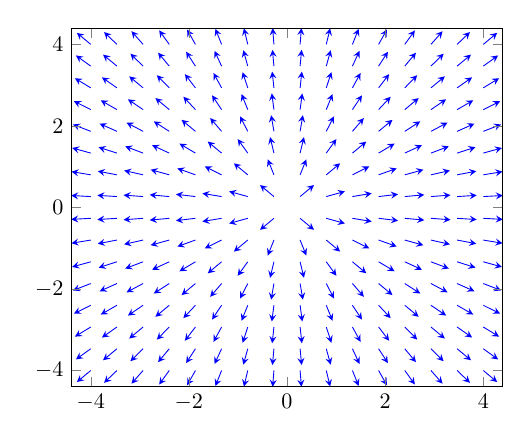
\begin{tikzpicture}[scale=0.8]
  \begin{axis}[view={0}{90}, domain=-4:4]
  \addplot3 [blue,-stealth,samples=16,
          quiver={
              u={2*x/pow(x^2 + y^2,1/2)},
              v={2*y/pow(x^2 + y^2,1/2)},
              scale arrows=0.2,
          },
      ] { 1};
  \end{axis}
  \end{tikzpicture}
  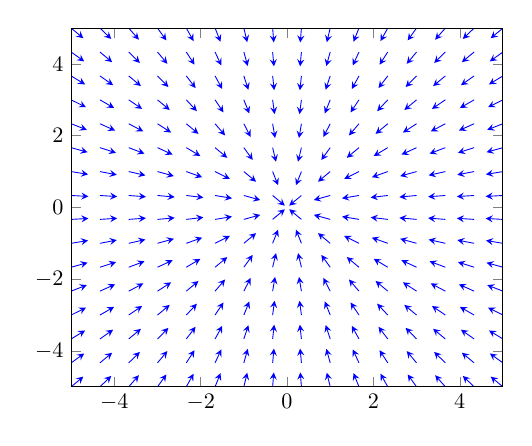
\begin{tikzpicture}[scale=0.8]
  \begin{axis}[view={0}{90}]
  \addplot3 [blue,-stealth,samples=16,
          quiver={
              u={-2*x/pow(x^2 + y^2,1/2)},
              v={-2*y/pow(x^2 + y^2,1/2)},
              scale arrows=0.2,
          },
      ] { 1};
  \end{axis}
  \end{tikzpicture}
  \end{center}
  \end{example}

  \begin{lemma}[Divergence in Cylindrical Coordinates]
  For vector field $F: \mathbb{R}^3 \longrightarrow \mathbb{R}^3$ expressed in cylindrical coordinates as 
  \[F = \begin{pmatrix}
  F_r \\ F_\theta \\ F_z
  \end{pmatrix}\]
  the divergence is
  \[\Div F = \nabla \cdot F = \frac{1}{r} \frac{\partial}{\partial r} \big(r F_r \big) + \frac{1}{r} \frac{\partial F_\theta}{\partial \theta} + \frac{\partial F_z}{\partial z}\]
  Note that the condition of locality is important, since in general a global cylindrical coordinate system would be inconsistent. 
  \end{lemma}

  \begin{lemma}[Divergence in Spherical Coordinates]
  For vector field $F: \mathbb{R}^3 \longrightarrow \mathbb{R}^3$ expressed in spherical coordinates $(r, \theta, \phi)$, the divergence is 
  \[\Div F = \nabla \cdot F = \frac{1}{r^2} \frac{\partial}{\partial r} \big( r^2 F_r) + \frac{1}{r \, \sin{\theta}} \frac{\partial}{\partial \theta} \big( \sin{\theta} F_\theta\big) + \frac{1}{r\, \sin{\theta}} \frac{\partial F_\phi}{\partial \phi}\]
  \end{lemma}

\subsection{Curl}

  Colloquially, the curl is a vector operator that describes the infinitesimal circulation of a vector field in $3$-dimensional Euclidean space, where the curl at each point is represented by a vector whose length and direction denote the magnitude and axis as the maximum circulation. That is, if one drops a twig or a ball with its center of mass at a certain point, the curl measures how much it will spin. In physics, the rotation of a rigid body in 3-dimensions can be described by a vector $\omega$ along the axis of rotation. $\omega$ is called the \textit{angular velocity vector}, with $||\omega||$ denoting the angular speed of the body. The curl of this vector field measured at the center of mass of the body is measured as $2 \omega$. That is, the curl outputs \textit{twice} the angular velocity vector of any rigid body. Note that unlike the gradient and divergence operators, curl does not generalize as simply to other dimensions. 

  \begin{definition}[Curl]
  The \textit{curl} of a 3-dimensional $C^k$ vector field $F: \mathbb{R}^3 \longrightarrow \mathbb{R}^3$ is an operator
  \[\curl: C^k (\mathbb{R}^3; \mathbb{R}^3) \longrightarrow C^{k-1} (\mathbb{R}^3; \mathbb{R}^3)\]
  defined
  \[\curl{F} \equiv \nabla \times F \equiv \begin{pmatrix}
  \frac{\partial}{\partial x} \\ \frac{\partial}{\partial y}\\ \frac{\partial}{\partial z} \end{pmatrix} \equiv \begin{pmatrix}
  \frac{\partial F_3}{\partial y} - \frac{\partial F_2}{\partial z} \\
  \frac{\partial F_1}{\partial z} - \frac{\partial F_3}{\partial x} \\
  \frac{\partial F_2}{\partial x} - \frac{\partial F_1}{\partial y}
  \end{pmatrix}\]
  \end{definition}

  \begin{definition}[Irrotational Vector Fields]
  A vector field $F$ is \textit{irrotational} if 
  \[\curl{F} = \mathbf{0}\]
  Visually, this indicates that there are no "whirlpools" everywhere, meaning that any rigid body placed anywhere, while it may travel along a path, will not rotate around its own axis. 
  \end{definition}

  It has been shown that fluid draining from a tub is usually irrotational except for right at the center, which is surprising since the fluid itself is "rotating" around the drain. 

  \begin{theorem}
  For any $C^2$ vector field $F$, 
  \[\Div{\curl{F}} = \nabla\cdot (\nabla \times F) = 0\]
  That is, the divergence of any curl is 0. 
  \end{theorem}
  \begin{proof}
  Proved by equality of mixed partials. 
  \end{proof}

  \begin{definition}
  The \textit{Laplace operator}, or \textit{Laplacian}, of a function $f: \mathbb{R}^n \longrightarrow \mathbb{R}$ is the divergence of the gradient. 
  \[\nabla^2 f \equiv \nabla \cdot (\nabla f) \equiv \sum_{i=1}^n \frac{\partial^2 f}{\partial x_i^2}\]
  \end{definition}

\subsection{Conservative, Solenoidal Vector Fields}

  \begin{definition}[Conservative Vector Fields]
  A vector field $F: U \subset \mathbb{R}^n \longrightarrow \mathbb{R}^n$ is a \textit{conservative vector field} if and only if there exists a scalar field $f: U \subset \mathbb{R}^n \longrightarrow \mathbb{R}$ such that 
  \[F = \nabla f\]
  on $U$. 
  \end{definition}

  Conservative vector fields appear naturally in mechanics: they are vector fields representing forces of physical systems in which energy is conserved. 

  \begin{theorem}
  Given a $C^2$-function $f: \mathbb{R}^3 \longrightarrow \mathbb{R}$,
  \[\nabla \times ( \nabla f) = 0\]
  That is, the curl of any gradient vector field is the zero vector. 
  \end{theorem}
  \begin{proof}
  $\nabla \times \nabla f$ can be expanded to
  \[\bigg( \frac{\partial^2 f}{\partial y \partial z} - \frac{\partial^2 f}{\partial z \partial y}, \; \frac{\partial^2 f}{\partial z \partial x} - \frac{\partial^2 f}{\partial x \partial z}, \; \frac{\partial^2 f}{\partial x \partial y} - \frac{\partial^2 f}{\partial y \partial x}\bigg) = (0, 0, 0)\]
  by equality of mixed partials. 
  \end{proof}

  \begin{definition}[Solenoidal Vector Fields]
  A \textit{solenoidal, or incompressible, vector field} is a vector field $F: \mathbb{R}^n \longrightarrow \mathbb{R}^n$ such that
  \[\Div F = \nabla \cdot F = 0\]
  at all point in the field. That is, the field has no sources or sinks. 
  \end{definition}

  \begin{example}
  The vector field $F: (x, y) \mapsto (y, -x)$ is solenoidal. 
  \begin{center}
      \includegraphics[scale=0.17]{img/Solenoidal_vector_field.png}
  \end{center}
  \end{example}


\section{Riemann Integration} 

  We would like to define an integral. We do this essentially by defining the Riemann sums for a particular partition, which is a number in $\mathbb{R}$. If we consider the set of all such Riemann sums, somehow bound them in a way. Then we define the upper and lower Riemann sums, and then consider the set of all Riemann sums. By doing so, we can construct two sets that are lower bounded and

  \begin{definition}[Partition]
    Let $[a, b]$ be an interval. A \textbf{partition} $P$ of $[a, b]$ is a set of $P = \{x_0, \ldots, x_n\}$ (note that this is finite!) s.t. 
    \begin{equation}
      a = x_0 \leq x_1 \leq \ldots \leq x_{n-1} \leq x_n = b
    \end{equation}
    with $\Delta x_i = x_i - x_{i-1}$ for $i = 1, \ldots, n$. 
  \end{definition}

  In some textbooks, we also define a \textit{partition with distinguished points} which simply is a partition $P$ along with some set of $\xi_i$'s that land in each interval. This allows for extra degrees of freedom for choosing points.  

  The natural way to define the Riemann integral is as the limit of the finite Riemann sums as partitions gets finer and finer.  But we must be careful in saying what ``finer'' means. It is not simply as the number of partitions $n \rightarrow \infty$, since this may lead to multiple subsequential values of convergence by increasing the partition within different subsets of $[a,b]$. 

  \begin{figure}[H]
    \centering
    % First row - upper sequence (red)
    \begin{subfigure}[b]{0.32\textwidth}
      \centering
      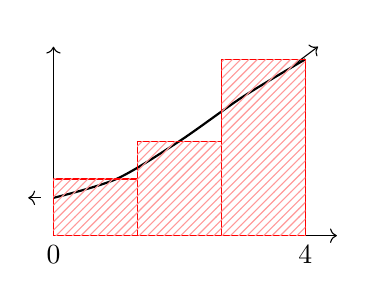
\begin{tikzpicture}[scale=0.8]
        % Axes
        \draw[->] (0,0) -- (4.5,0) node[right] {};
        \draw[->] (0,0) -- (0,3) node[above] {};
        
        % Origin label
        \node[below] at (0,0) {$0$};
        \node[below] at (4,0) {$4$};
        
        % Function curve
        \draw[thick] plot[domain=0:4, samples=100, smooth] coordinates {(0,0.6) (1,0.9) (2,1.5) (3,2.2) (4,2.8)};
        
        % Arrow at left end of curve
        \draw[->] (-0.2,0.6) -- (-0.4,0.6);
        % Arrow at right end of curve
        \draw[->] (3.8,2.7) -- (4.2,3.0);
        
        % Rectangles and patterns - rightmost is fixed
        \draw[red] (0,0) rectangle (1.33,0.9);
        \draw[red] (1.33,0) rectangle (2.67,1.5);
        \draw[red] (2.67,0) rectangle (4,2.8);
        
        % Fill with diagonal pattern
        \fill[pattern=north east lines, pattern color=red!40] (0,0) rectangle (1.33,0.9);
        \fill[pattern=north east lines, pattern color=red!40] (1.33,0) rectangle (2.67,1.5);
        \fill[pattern=north east lines, pattern color=red!40] (2.67,0) rectangle (4,2.8);
      \end{tikzpicture}
      \caption{}
    \end{subfigure}
    \hfill 
    \begin{subfigure}[b]{0.32\textwidth}
      \centering
      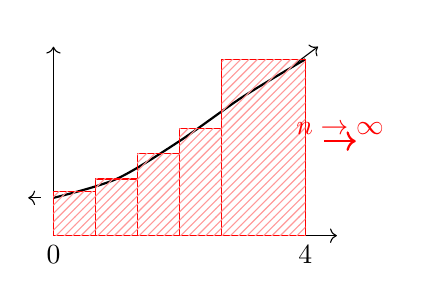
\begin{tikzpicture}[scale=0.8]
        % Axes
        \draw[->] (0,0) -- (4.5,0) node[right] {};
        \draw[->] (0,0) -- (0,3) node[above] {};
        
        % Origin label
        \node[below] at (0,0) {$0$};
        \node[below] at (4,0) {$4$};
        
        % Function curve
        \draw[thick] plot[domain=0:4, samples=100, smooth] coordinates {(0,0.6) (1,0.9) (2,1.5) (3,2.2) (4,2.8)};
        
        % Arrow at left end of curve
        \draw[->] (-0.2,0.6) -- (-0.4,0.6);
        % Arrow at right end of curve
        \draw[->] (3.8,2.7) -- (4.2,3.0);
        
        % Rectangles and patterns - rightmost is fixed
        \draw[red] (0,0) rectangle (0.67,0.7);
        \draw[red] (0.67,0) rectangle (1.33,0.9);
        \draw[red] (1.33,0) rectangle (2,1.3);
        \draw[red] (2,0) rectangle (2.67,1.7);
        \draw[red] (2.67,0) rectangle (4,2.8);
        
        % Fill with diagonal pattern
        \fill[pattern=north east lines, pattern color=red!40] (0,0) rectangle (0.67,0.7);
        \fill[pattern=north east lines, pattern color=red!40] (0.67,0) rectangle (1.33,0.9);
        \fill[pattern=north east lines, pattern color=red!40] (1.33,0) rectangle (2,1.3);
        \fill[pattern=north east lines, pattern color=red!40] (2,0) rectangle (2.67,1.7);
        \fill[pattern=north east lines, pattern color=red!40] (2.67,0) rectangle (4,2.8);
        
        % Red arrow showing refinement
        \draw[->, red, thick] (4.3,1.5) -- (4.8,1.5);
        \node[red] at (4.55,1.7) {$n\to\infty$};
      \end{tikzpicture}
      \caption{}
    \end{subfigure}
    \hfill 
    \begin{subfigure}[b]{0.32\textwidth}
      \centering
      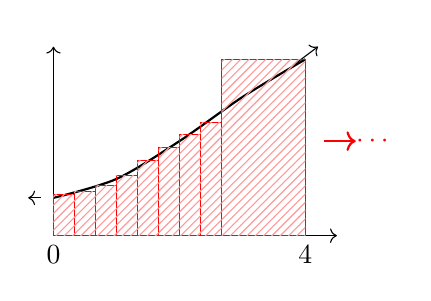
\begin{tikzpicture}[scale=0.8]
        % Axes
        \draw[->] (0,0) -- (4.5,0) node[right] {};
        \draw[->] (0,0) -- (0,3) node[above] {};
        
        % Origin label
        \node[below] at (0,0) {$0$};
        \node[below] at (4,0) {$4$};
        
        % Function curve
        \draw[thick] plot[domain=0:4, samples=100, smooth] coordinates {(0,0.6) (1,0.9) (2,1.5) (3,2.2) (4,2.8)};
        
        % Arrow at left end of curve
        \draw[->] (-0.2,0.6) -- (-0.4,0.6);
        % Arrow at right end of curve
        \draw[->] (3.8,2.7) -- (4.2,3.0);
        
        % Rectangles and patterns - rightmost is fixed
        \draw[red] (0,0) rectangle (0.33,0.65);
        \draw[red] (0.33,0) rectangle (0.67,0.7);
        \draw[red] (0.67,0) rectangle (1,0.8);
        \draw[red] (1,0) rectangle (1.33,0.95);
        \draw[red] (1.33,0) rectangle (1.67,1.2);
        \draw[red] (1.67,0) rectangle (2,1.4);
        \draw[red] (2,0) rectangle (2.33,1.6);
        \draw[red] (2.33,0) rectangle (2.67,1.8);
        \draw[red] (2.67,0) rectangle (4,2.8);
        
        % Fill with diagonal pattern
        \fill[pattern=north east lines, pattern color=red!40] (0,0) rectangle (0.33,0.65);
        \fill[pattern=north east lines, pattern color=red!40] (0.33,0) rectangle (0.67,0.7);
        \fill[pattern=north east lines, pattern color=red!40] (0.67,0) rectangle (1,0.8);
        \fill[pattern=north east lines, pattern color=red!40] (1,0) rectangle (1.33,0.95);
        \fill[pattern=north east lines, pattern color=red!40] (1.33,0) rectangle (1.67,1.2);
        \fill[pattern=north east lines, pattern color=red!40] (1.67,0) rectangle (2,1.4);
        \fill[pattern=north east lines, pattern color=red!40] (2,0) rectangle (2.33,1.6);
        \fill[pattern=north east lines, pattern color=red!40] (2.33,0) rectangle (2.67,1.8);
        \fill[pattern=north east lines, pattern color=red!40] (2.67,0) rectangle (4,2.8);
        
        % Red arrow showing refinement with dots
        \draw[->, red, thick] (4.3,1.5) -- (4.8,1.5);
        \node[red] at (5.1,1.5) {$\cdots$};
      \end{tikzpicture}
      \caption{}
    \end{subfigure}
    
    % Second row - lower sequence (blue)
    \begin{subfigure}[b]{0.32\textwidth}
      \centering
      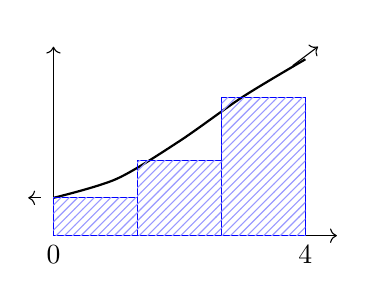
\begin{tikzpicture}[scale=0.8]
        % Axes
        \draw[->] (0,0) -- (4.5,0) node[right] {};
        \draw[->] (0,0) -- (0,3) node[above] {};
        
        % Origin label
        \node[below] at (0,0) {$0$};
        \node[below] at (4,0) {$4$};
        
        % Function curve
        \draw[thick] plot[domain=0:4, samples=100, smooth] coordinates {(0,0.6) (1,0.9) (2,1.5) (3,2.2) (4,2.8)};
        
        % Arrow at left end of curve
        \draw[->] (-0.2,0.6) -- (-0.4,0.6);
        % Arrow at right end of curve
        \draw[->] (3.8,2.7) -- (4.2,3.0);
        
        % Rectangles and patterns - leftmost is fixed
        \draw[blue] (0,0) rectangle (1.33,0.6);
        \draw[blue] (1.33,0) rectangle (2.67,1.2);
        \draw[blue] (2.67,0) rectangle (4,2.2);
        
        % Fill with diagonal pattern
        \fill[pattern=north east lines, pattern color=blue!40] (0,0) rectangle (1.33,0.6);
        \fill[pattern=north east lines, pattern color=blue!40] (1.33,0) rectangle (2.67,1.2);
        \fill[pattern=north east lines, pattern color=blue!40] (2.67,0) rectangle (4,2.2);
      \end{tikzpicture}
      \caption{}
    \end{subfigure}
    \hfill 
    \begin{subfigure}[b]{0.32\textwidth}
      \centering
      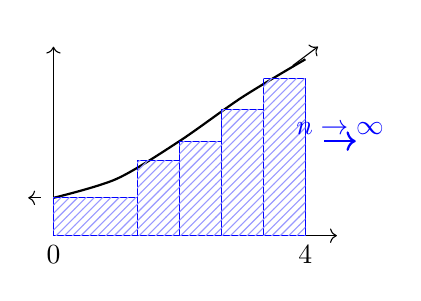
\begin{tikzpicture}[scale=0.8]
        % Axes
        \draw[->] (0,0) -- (4.5,0) node[right] {};
        \draw[->] (0,0) -- (0,3) node[above] {};
        
        % Origin label
        \node[below] at (0,0) {$0$};
        \node[below] at (4,0) {$4$};
        
        % Function curve
        \draw[thick] plot[domain=0:4, samples=100, smooth] coordinates {(0,0.6) (1,0.9) (2,1.5) (3,2.2) (4,2.8)};
        
        % Arrow at left end of curve
        \draw[->] (-0.2,0.6) -- (-0.4,0.6);
        % Arrow at right end of curve
        \draw[->] (3.8,2.7) -- (4.2,3.0);
        
        % Rectangles and patterns - leftmost is fixed
        \draw[blue] (0,0) rectangle (1.33,0.6);
        \draw[blue] (1.33,0) rectangle (2,1.2);
        \draw[blue] (2,0) rectangle (2.67,1.5);
        \draw[blue] (2.67,0) rectangle (3.33,2.0);
        \draw[blue] (3.33,0) rectangle (4,2.5);
        
        % Fill with diagonal pattern
        \fill[pattern=north east lines, pattern color=blue!40] (0,0) rectangle (1.33,0.6);
        \fill[pattern=north east lines, pattern color=blue!40] (1.33,0) rectangle (2,1.2);
        \fill[pattern=north east lines, pattern color=blue!40] (2,0) rectangle (2.67,1.5);
        \fill[pattern=north east lines, pattern color=blue!40] (2.67,0) rectangle (3.33,2.0);
        \fill[pattern=north east lines, pattern color=blue!40] (3.33,0) rectangle (4,2.5);
        
        % Blue arrow showing refinement
        \draw[->, blue, thick] (4.3,1.5) -- (4.8,1.5);
        \node[blue] at (4.55,1.7) {$n\to\infty$};
      \end{tikzpicture}
      \caption{}
    \end{subfigure}
    \hfill 
    \begin{subfigure}[b]{0.32\textwidth}
      \centering
      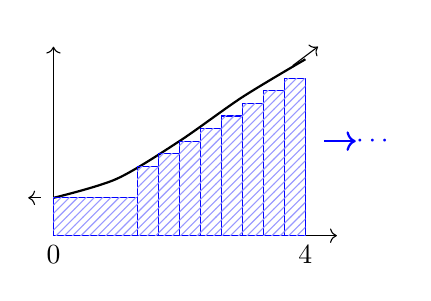
\begin{tikzpicture}[scale=0.8]
        % Axes
        \draw[->] (0,0) -- (4.5,0) node[right] {};
        \draw[->] (0,0) -- (0,3) node[above] {};
        
        % Origin label
        \node[below] at (0,0) {$0$};
        \node[below] at (4,0) {$4$};
        
        % Function curve
        \draw[thick] plot[domain=0:4, samples=100, smooth] coordinates {(0,0.6) (1,0.9) (2,1.5) (3,2.2) (4,2.8)};
        
        % Arrow at left end of curve
        \draw[->] (-0.2,0.6) -- (-0.4,0.6);
        % Arrow at right end of curve
        \draw[->] (3.8,2.7) -- (4.2,3.0);
        
        % Rectangles and patterns - leftmost is fixed
        \draw[blue] (0,0) rectangle (1.33,0.6);
        \draw[blue] (1.33,0) rectangle (1.67,1.1);
        \draw[blue] (1.67,0) rectangle (2,1.3);
        \draw[blue] (2,0) rectangle (2.33,1.5);
        \draw[blue] (2.33,0) rectangle (2.67,1.7);
        \draw[blue] (2.67,0) rectangle (3,1.9);
        \draw[blue] (3,0) rectangle (3.33,2.1);
        \draw[blue] (3.33,0) rectangle (3.67,2.3);
        \draw[blue] (3.67,0) rectangle (4,2.5);
        
        % Fill with diagonal pattern
        \fill[pattern=north east lines, pattern color=blue!40] (0,0) rectangle (1.33,0.6);
        \fill[pattern=north east lines, pattern color=blue!40] (1.33,0) rectangle (1.67,1.1);
        \fill[pattern=north east lines, pattern color=blue!40] (1.67,0) rectangle (2,1.3);
        \fill[pattern=north east lines, pattern color=blue!40] (2,0) rectangle (2.33,1.5);
        \fill[pattern=north east lines, pattern color=blue!40] (2.33,0) rectangle (2.67,1.7);
        \fill[pattern=north east lines, pattern color=blue!40] (2.67,0) rectangle (3,1.9);
        \fill[pattern=north east lines, pattern color=blue!40] (3,0) rectangle (3.33,2.1);
        \fill[pattern=north east lines, pattern color=blue!40] (3.33,0) rectangle (3.67,2.3);
        \fill[pattern=north east lines, pattern color=blue!40] (3.67,0) rectangle (4,2.5);
        
        % Blue arrow showing refinement with dots
        \draw[->, blue, thick] (4.3,1.5) -- (4.8,1.5);
        \node[blue] at (5.1,1.5) {$\cdots$};
      \end{tikzpicture}
      \caption{}
    \end{subfigure}
    
    \caption{Upper (top row) and lower (bottom row) Riemann sums with refinement of partition. In the upper row, the rightmost rectangle remains fixed while other rectangles become thinner. In the lower row, the leftmost rectangle remains fixed while other rectangles become thinner.}
    \label{fig:upper-lower-refinement}
  \end{figure}

  An alternative way is to have the partitions all converge ``uniformly'' as in the maximum length of an interval in a partition must go to $0$. 

  \begin{figure}[H]
    \centering
    \begin{subfigure}[b]{0.32\textwidth}
      \centering
      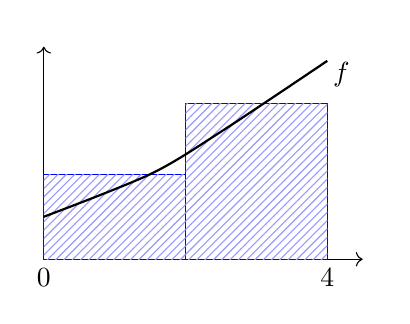
\begin{tikzpicture}[scale=0.9]
        % Axes
        \draw[->] (0,0) -- (4.5,0) node[right] {};
        \draw[->] (0,0) -- (0,3) node[above] {};
        
        % Origin label
        \node[below] at (0,0) {$0$};
        \node[below] at (4,0) {$4$};
        
        % Rectangles and patterns
        \draw[blue] (0,0) rectangle (2,1.2);
        \draw[blue] (2,0) rectangle (4,2.2);
        
        % Fill with diagonal pattern
        \fill[pattern=north east lines, pattern color=blue!40] (0,0) rectangle (2,1.2);
        \fill[pattern=north east lines, pattern color=blue!40] (2,0) rectangle (4,2.2);
        
        % Function curve
        \draw[thick] plot[domain=0:4, samples=100, smooth] coordinates {(0,0.6) (1.5,1.2) (2.5,1.8) (4,2.8)};
        
        % Label f (no arrow)
        \node at (4.2,2.6) {$f$};
      \end{tikzpicture}
      \caption{$\lambda(P) = 2$}
    \end{subfigure}
    \hfill 
    \begin{subfigure}[b]{0.32\textwidth}
      \centering
      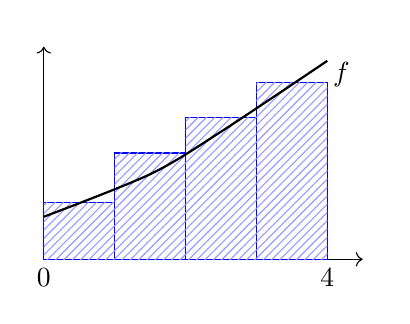
\begin{tikzpicture}[scale=0.9]
        % Axes
        \draw[->] (0,0) -- (4.5,0) node[right] {};
        \draw[->] (0,0) -- (0,3) node[above] {};
        
        % Origin label
        \node[below] at (0,0) {$0$};
        \node[below] at (4,0) {$4$};
        
        % Rectangles and patterns
        \draw[blue] (0,0) rectangle (1,0.8);
        \draw[blue] (1,0) rectangle (2,1.5);
        \draw[blue] (2,0) rectangle (3,2);
        \draw[blue] (3,0) rectangle (4,2.5);
        
        % Fill with diagonal pattern
        \fill[pattern=north east lines, pattern color=blue!40] (0,0) rectangle (1,0.8);
        \fill[pattern=north east lines, pattern color=blue!40] (1,0) rectangle (2,1.5);
        \fill[pattern=north east lines, pattern color=blue!40] (2,0) rectangle (3,2);
        \fill[pattern=north east lines, pattern color=blue!40] (3,0) rectangle (4,2.5);
        
        % Function curve
        \draw[thick] plot[domain=0:4, samples=100, smooth] coordinates {(0,0.6) (1.5,1.2) (2.5,1.8) (4,2.8)};
        
        % Label f (no arrow)
        \node at (4.2,2.6) {$f$};
      \end{tikzpicture}
      \caption{$\lambda(P) = 1$}
    \end{subfigure}
    \hfill 
    \begin{subfigure}[b]{0.32\textwidth}
      \centering
      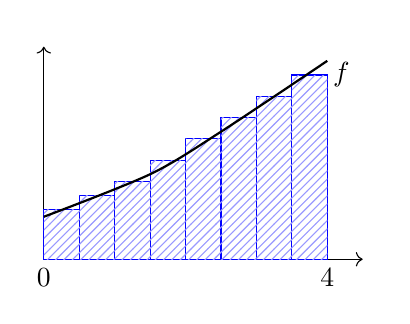
\begin{tikzpicture}[scale=0.9]
        % Axes
        \draw[->] (0,0) -- (4.5,0) node[right] {};
        \draw[->] (0,0) -- (0,3) node[above] {};
        
        % Origin label
        \node[below] at (0,0) {$0$};
        \node[below] at (4,0) {$4$};
        
        % Rectangles and patterns
        \draw[blue] (0,0) rectangle (0.5,0.7);
        \draw[blue] (0.5,0) rectangle (1,0.9);
        \draw[blue] (1,0) rectangle (1.5,1.1);
        \draw[blue] (1.5,0) rectangle (2,1.4);
        \draw[blue] (2,0) rectangle (2.5,1.7);
        \draw[blue] (2.5,0) rectangle (3,2);
        \draw[blue] (3,0) rectangle (3.5,2.3);
        \draw[blue] (3.5,0) rectangle (4,2.6);
        
        % Fill with diagonal pattern
        \fill[pattern=north east lines, pattern color=blue!40] (0,0) rectangle (0.5,0.7);
        \fill[pattern=north east lines, pattern color=blue!40] (0.5,0) rectangle (1,0.9);
        \fill[pattern=north east lines, pattern color=blue!40] (1,0) rectangle (1.5,1.1);
        \fill[pattern=north east lines, pattern color=blue!40] (1.5,0) rectangle (2,1.4);
        \fill[pattern=north east lines, pattern color=blue!40] (2,0) rectangle (2.5,1.7);
        \fill[pattern=north east lines, pattern color=blue!40] (2.5,0) rectangle (3,2);
        \fill[pattern=north east lines, pattern color=blue!40] (3,0) rectangle (3.5,2.3);
        \fill[pattern=north east lines, pattern color=blue!40] (3.5,0) rectangle (4,2.6);
        
        % Function curve
        \draw[thick] plot[domain=0:4, samples=100, smooth] coordinates {(0,0.6) (1.5,1.2) (2.5,1.8) (4,2.8)};
        
        % Label f (no arrow)
        \node at (4.2,2.6) {$f$};
      \end{tikzpicture}
      \caption{$\lambda(P) = 0.5$}
    \end{subfigure}
    \caption{Approximating an integral with increasingly fine partitions}
    \label{fig:partition-refinement}
  \end{figure}

  A cleaner way it to simply look at the set of all partitions along with the set of the corresponding upper and lower Riemann sums, and then hope that they behave nicely with each other. This is the approach we will take. 

  \begin{definition}[Riemann Sums with Respect to Partition]
    Let $P$ be a partition of $[a, b]$ and $f: [a, b] \to \mathbb{R}$ be bounded. Then, the \textbf{upper and lower Riemann sum} is defined 
    \begin{equation}
      M_i = \sup_{\Delta x_i} f(x), \qquad m_i = \inf_{\Delta x_i} f(x) 
    \end{equation}
    Now define  
    \begin{equation}
      U(P, f) = \sum_{i=1}^n M_i \Delta x_i, \qquad L(P, f) = \sum_{i=1}^n m_i \Delta x_i
    \end{equation}

    \begin{figure}[H]
      \centering 
      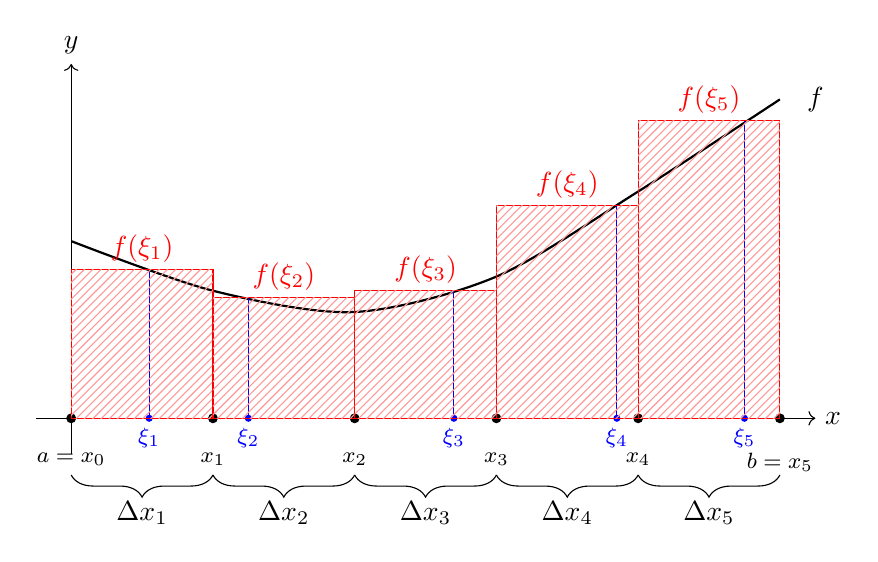
\begin{tikzpicture}[scale=0.9]
        % Define axes
        \draw[->] (-0.5,0) -- (10.5,0) node[right] {$x$};
        \draw[->] (0,-0.5) -- (0,5) node[above] {$y$};
        
        % Function curve
        \draw[thick] plot[domain=0:10, samples=100, smooth] 
            coordinates {(0,2.5) (2,1.8) (4,1.5) (6,2) (8,3.2) (10,4.5)};
        
        % f label
        \node at (10.5,4.5) {$f$};
        
        % Partition points on x-axis
        \foreach \x/\label [count=\i from 0] in {
          0/a=x_0, 2/x_1, 4/x_2, 6/x_3, 8/x_4, 10/b=x_5
        } {
          \fill (\x,0) circle (0.07);
          \node[black, below, font=\footnotesize] at (\x,-0.35) {$\label$};
        }
        
        % Sample points ξᵢ (blue)
        \foreach \x/\label [count=\i from 1] in {
          1.1/\xi_1, 2.5/\xi_2, 5.4/\xi_3, 7.7/\xi_4, 9.5/\xi_5
        } {
          \fill[blue] (\x,0) circle (0.05);
          \node[blue, below, font=\footnotesize] at (\x,0) {$\label$};
          
        }
        \draw[blue, thin] (1.1,0) -- (1.1,2.1);
        \draw[blue, thin] (2.5,0) -- (2.5,1.7);
        \draw[blue, thin] (5.4,0) -- (5.4,1.8);
        \draw[blue, thin] (7.7,0) -- (7.7,3);
        \draw[blue, thin] (9.5,0) -- (9.5,4.2);
        
        % Rectangles for Riemann sum
        \foreach \xstart/\xend/\y [count=\i from 1] in {
          0/2/2.1, 2/4/1.7, 4/6/1.8, 6/8/3, 8/10/4.2
        } {
          % Rectangle with red border and pattern
          \draw[red] (\xstart,0) rectangle (\xend,\y);
          \fill[pattern=north east lines, pattern color=red!40] (\xstart,0) rectangle (\xend,\y);
          
          % Function value labels
          \node[red] at ({(\xstart+\xend)/2},{\y+0.3}) {$f(\xi_{\i})$};
        }
        
        % Delta x labels with curly braces (opening downward)
        \foreach \xstart/\xend/\i in {
          0/2/1, 2/4/2, 4/6/3, 6/8/4, 8/10/5
        } {
          \draw[decorate, decoration={brace, mirror, amplitude=8pt}, black] 
            (\xstart,-0.8) -- (\xend,-0.8) node[midway, below, yshift=-6pt] {$\Delta x_{\i}$};
        }
      \end{tikzpicture}
      \caption{Riemann sum approximation using sample points $\xi_i$ within each subinterval. This is known as a Riemann sum of a partition with distinguished points. The Riemann sum is a mapping that takes in a partition with distinguished points $p = (P, \xi)$ on the closed interval $[a, b]$ and outputs a number representing the total area of the Riemann sums. }
      \label{fig:riemann-sum-xi}
    \end{figure}
  \end{definition}

  \begin{definition}[Riemann Integral]
    Now, given the same assumptions, the \textbf{upper and lower Rimemann integrals} of $f(x)$ are defined 
    \begin{equation}
      \int_a^{\bar{b}} f(x) \, dx \coloneqq \inf_P U(P, f), \qquad \int_{\bar{a}}^{b} f(x) \, dx \coloneqq \sup_P L(P, f)
    \end{equation}
    If the upper and lower Riemann integrals are equal, then $f$ is said to be \textbf{Riemann integrable} over $[a, b]$, denoted $f \in \mathcal{R}([a, b])$.\footnote{Where $\mathcal{R}(X)$ is the set of all Riemann integrable functions over $X$.}
  \end{definition} 

  Great, so we've defined Riemann integrable functions, but it's hard to determine whether a function is Riemann integrable---and if so---what the value of the integral is. We will determine the first problem by talking about sufficient conditions for Riemann integrability, and then introduce the fundamental theorem of calculus to address computability. 

  \begin{definition}[Refinement]
    $P^\ast$ is a \textbf{refinement} of $P$ if $P \subset P^\ast$. If $P_1, P_2$ are two partitions, then their \textbf{common refinement} $P^\ast = P_1 \cup P_2$. 

    \begin{figure}[H]
      \centering 
      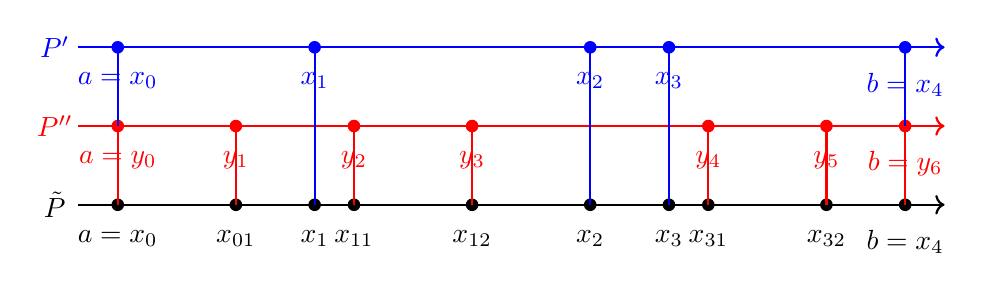
\begin{tikzpicture}[scale=1.0]
        % First partition P' (blue) - reduced vertical spacing
        \draw[thick, blue, ->] (-0.5,1) -- (10.5,1);
        \node[blue] at (-0.8,1) {$P'$};
        
        % Points on first partition
        \foreach \x/\label [count=\i from 0] in {
          0/a=x_0, 2.5/x_1, 6/x_2, 7/x_3, 10/b=x_4
        } {
          \fill[blue] (\x,1) circle (0.08);
          \node[blue, below] at (\x,0.8) {$\label$};
        }
        
        % Second partition P'' (red) - reduced vertical spacing
        \draw[thick, red, ->] (-0.5,0) -- (10.5,0);
        \node[red] at (-0.8,0) {$P''$};
        
        % Points on second partition
        \foreach \x/\label [count=\i from 0] in {
          0/a=y_0, 1.5/y_1, 3/y_2, 4.5/y_3, 7.5/y_4, 9/y_5, 10/b=y_6
        } {
          \fill[red] (\x,0) circle (0.08);
          \node[red, below] at (\x,-0.2) {$\label$};
        }
        
        % Third partition P̃ (black) - combined partition - reduced vertical spacing
        \draw[thick, ->] (-0.5,-1) -- (10.5,-1);
        \node at (-0.8,-1) {$\tilde{P}$};
        
        % Points on combined partition - all points from both partitions
        \foreach \x/\label [count=\i from 0] in {
          0/a=x_0, 1.5/x_{01}, 2.5/x_1, 3/x_{11}, 4.5/x_{12}, 6/x_2, 7/x_3, 7.5/x_{31}, 9/x_{32}, 10/b=x_4
        } {
          \fill (\x,-1) circle (0.08);
          \node[below] at (\x,-1.2) {$\label$};
        }
        
        % Vertical lines connecting corresponding points
        % From P' to P̃
        \foreach \x in {0, 2.5, 6, 7, 10} {
          \draw[blue, thick] (\x,1) -- (\x,-1);
        }
        
        % From P'' to P̃
        \foreach \x in {0, 1.5, 3, 4.5, 7.5, 9, 10} {
          \draw[red, thick] (\x,0) -- (\x,-1);
        }
      \end{tikzpicture}
      \caption{Partitions $P'$ and $P''$ with their common refinement $\tilde{P}$}
      \label{fig:three-partitions}
    \end{figure}
  \end{definition}

  \begin{lemma}[Fundamental Lemma]
    If $P^\ast$ is a refinement of $P$ and $f: [a, b] \to \mathbb{R}$ is bounded, then 
    \begin{equation}
      L(P, f) \leq L(P^\ast, F) \leq U(P^\ast, F) \leq U(P, f) 
    \end{equation}
  \end{lemma}
  \begin{proof} 
    By induction on the number of points we add to $P$ to get $P^\ast$, we might as well assume that $P^\ast = P \cup \{x_\ast\}$. So, 
    \begin{align}
      P & = \{a = x_0, x_1, \ldots, x_{n-1}, x_n \} \\
      P^\ast & = \{a = x_0, x_1, \ldots, x_{i-1}, x_i, x_\ast, x_{i+1}, \ldots, x_{n-1}, x_n \} \\
    \end{align}
    Now let's compute $L(f, P^\ast) - L(f, P)$. Since the only intervals affected are $[x_i, x_{i+1}]$, we have 
    \begin{align}
      L(f, P^\ast) - L(f, P) & = \inf_{[x_i, x_{\ast}]} f(x) (x_{\ast} - x_i) + \inf_{[x_\ast, x_{i+1}]} f(x) (x_{i+1} - x_\ast) - \inf_{[x_{i}, x_{i+1}]} f(x) (x_{i+1} - x_i) \\ 
                             & = \big( \underbrace{\inf_{[x_i, x_{\ast}]} f(x) - \inf_{[x_{\ast}, x_{i+1}]} f(x)}_{> 0} \big) (x_\ast - x_i) + \big( \underbrace{\inf_{[x_\ast, x_{i+1}]} f(x) - \inf_{[x_i , x_{i+1}]}}_{> 0} \big) (x_{i+1} - x_\ast) 
    \end{align}
    which is therefore greater than $0$. 
  \end{proof}

  \begin{theorem}[Lower and Upper Integrals as Bounds of Each Other]
    We claim
    \begin{equation}
      \int_{\bar{a}}^b f(x) \, dx \leq \int_{a}^{\bar{b}} f(x) \, dx
    \end{equation}
  \end{theorem}
  \begin{proof}
    Given $P_1, P_2$ partitions, let $P^\ast = P_1 \cup P_2$ be their common refinement. Then, from the theorem above, 
    \begin{equation}
      L(P_2, f) \leq L(P^\ast, f) \leq U(P^\ast, f) \leq U(P, f) 
    \end{equation}
    So taking the supremum over all partitions $P_2$ and fixing $P_1$ gives 
    \begin{equation}
      \int_{\bar{a}}^b f(x) \, dx = \sup_{P_2} L(P_2, f) \leq \sup_{P_2} U(P_1, f) = U(P_1, f)
    \end{equation}
    Then taking the infimum over all partitions $P_1$ gives us 
    \begin{equation}
      \int_{\bar{a}}^b f(x) \, dx = \inf_{P_1} \int_{\bar{a}}^b f(x) \, dx \leq \inf_{P_1} U(P_1, f) = \int_{a}^{\bar{b}} f(x) \,dx
    \end{equation}
    where we note that the infimum does not affect the terms that do not depend on $P_1$. 
  \end{proof}

\subsection{Conditions for Integrability}

  We have seen some bounds of the upper and lower integrals, and defined the Riemann integral. However, checking Riemann integrability is quite tedious, since we have to take the supremum and infimum over all possible partitions. The following theorem is extremely useful as it only requires us to find \textit{one} partition given some $\epsilon$. In some sense, this is similar to the Cauchy convergence criterion. 

  \begin{theorem}[Cauchy]
    $f \in \mathcal{R}$ iff $\forall \epsilon > 0$, there exists partition $P$ such that $U(P, f) - L(P, f) < \epsilon$. 
  \end{theorem}
  \begin{proof}
    We prove bidirectionally. The reverse implication is easy, but for the forward direction you must use refinements. 
    \begin{enumerate}
      \item $(\leftarrow)$. Pick any partition $P$. Since
        \begin{align}
          L(f, P) \leq \int_{\bar{a}}^b f(x) \, dx \leq \int_a^{\bar{b}} f(x)\,dx \leq U(f, P)
        \end{align}
        This implies that 
        \begin{equation}
          0 \leq \int_a^{\bar{b}} f(x)\,dx - \int_{\bar{a}}^b f(x) \, dx \leq U(f, P) - L(f, P) < \epsilon 
        \end{equation}
        and since any nonnegative number less than any positive number must be $0$ (since there are no infinitesimals in $\mathbb{R}$), the LHS is $0$, and the result is proven.  

      \item $(\rightarrow)$. $f$ is Riemann integrable, so  
        \begin{equation}
          \int_a^{\bar{b}} f(x) \,dx = \int_{\bar{a}}^{b} f(x) \,dx \iff \inf_P U(f, P) = \sup_{Q} L(f, Q) 
        \end{equation}
        for partitions $P, Q$. So we can find $P$ that gets really close to the infimum and same for $Q$ close to the supremum, i.e. there exists a $P, Q$, such that
        \begin{equation}
          U(f, P) < \int_a^{\bar{b}} f(x) \,dx + \frac{\epsilon}{2}, \qquad L(f, Q) > \int_{\bar{a}}^b f(x) \,dx - \frac{\epsilon}{2}
        \end{equation}
        Now take the common refinement $P^\ast = P \cup Q$, and so by the fundamental lemma, 
        \begin{equation}
          \int_{\bar{a}}^b f(x) \,dx - \frac{\epsilon}{2} < L(f, Q) \leq L(f, P^\ast) \leq U(f, P^\ast) \leq U(f, P) < \int_a^{\bar{b}} f(x) \,dx + \frac{\epsilon}{2}
        \end{equation} 
        which implies that $0 \leq U(f, P^\ast) - L(f, P^\ast) < \epsilon$. 
    \end{enumerate}
  \end{proof}  

  Note that a necessary condition of $f$ being Riemann integrable is that $f$ is bounded. In fact it is defined that way. You may know that a sufficient condition of integrability is that it is continuous, but we can prove something slightly weaker. 

  \begin{definition}[Oscillation]
    Given an interval $I$, the \textbf{oscillation} of $f$ on $I$ is defined 
    \begin{equation}
      \mathop{\osc}_{I} (f) \coloneqq \sup_I (f) - \inf_I (f)
    \end{equation}
  \end{definition}

  Intuitively, a function $f$ is Riemann integrable if we can make $U(f, P) - L(f, P)$ as small as we wish. This is the case if we can find a sufficiently refined partition $P$ such that the oscillation on $f$ on each interval is small. 

  \begin{lemma}[Functions with Vanishing Osillations are Riemann Integrable]
    Let $f$ be a bounded on a closed interval $[a, b]$. If, for every $\epsilon > 0$, there exists a partition $P$ such that
    \begin{equation}
      \sum_{i=0}^{n-1} \mathop{\osc}_{[x_i, x_{i+1}]} f < \epsilon
    \end{equation}
    then $f$ is Riemann integrable. 
  \end{lemma}
  \begin{proof}
    Given $\epsilon > 0$, choose $\epsilon/(b-a)$. By assumption we can find a partition $P$ in which the total oscillation is bounded above by $\epsilon/(b-a)$. Therefore, 
    \begin{align}
      U(P, f) - L(P, f) & = \sum_{i=0}^{n-1} \sup_{[x_i, x_{i+1}]} f(x) \Delta x_i - \sum_{i=0}^{n-1} \inf_{[x_i, x_{i+1}]} f(x) \Delta x_i \\ 
                        & = \sum_{i=0}^{n-1} (\sup_{[x_i, x_{i+1}]} f(x) - \inf_{[x_i, x_{i+1}]} f(x) ) \Delta x_i \\ 
                        & < \sum_{i=0}^{n-1} \mathop{\osc}_{[x_i, x_{i+1}]} f \Delta x_i \\ 
                        & \leq \sum_{i=0}^{n-1} \frac{\epsilon}{b-a} \Delta x_i \\ 
                        & = \frac{\epsilon}{b-a} \sum_{i=0}^{n-1} \Delta x_i \\
                        & = \frac{\epsilon}{b-a} (b-a) = \epsilon
    \end{align}
  \end{proof} 

  Here is a classic example of a non-integrable function.  

  \begin{example}[Non-Integrability of the Dirichlet Function]
    The Dirichlet function
    \begin{equation}
      \mathcal{D}(x) \equiv \begin{cases}
        1, & \text{ for } x \in \mathbb{Q} \\
        0, & \text{ for } x \in \mathbb{R} \setminus \mathbb{Q}
      \end{cases}
    \end{equation}
    on the interval $[0,1]$ is not integrable on that interval. For any partition $P$ of $[0,1]$ we can find in each interval $\Delta_i$ both a rational point $\xi^\prime_i$ and an irrational point $\xi_i^{\prime\prime}$. Then, we can see that the lower and upper Riemann sums do not necessarily converge to each other since
    \begin{equation}
      \sigma(f; P, \xi^\prime) = \sum_{i=1}^n 1 \cdot \Delta x_i = 1 \text{ while } \sigma(f;P, \xi^{\prime\prime}) = \sum_{i=1}^n 0 \cdot \Delta x_i = 0
    \end{equation}
    as $\lambda(P) \rightarrow 0$. 
  \end{example}

  \begin{example}
    Is there a function $f$ that is discontinuous on a dense set of $[0, 1]$ but still Riemann integrable? 
  \end{example}

  With this, we can use the uniform continuity of continuous functions over a compact set to place a bound on the oscillation of each subinterval---and thus a bound on the oscillation of the whole interval. 

  \begin{theorem}[Continuous Functions are Riemann Integrable]
    $f$ continuous on $[a, b] \implies f$ is Riemann integrable on $[a, b]$. 
  \end{theorem}
  \begin{proof}
    If $f$ is continuous, then by EVT it is bounded and uniformly continuous. Therefore we can take the evenly-partitioned intervals of $[a, b]$ and by uniform continuity, the oscillation tends to $0$, and we are done. 

    Perhaps more explicitly, we wish to show that for all $\epsilon > 0$, there exists partition $P$ s.t. $U(P, f) - L(P, f) < \epsilon$. Now let $\epsilon > 0$, and since it's uniformly continuous, take $\delta > 0$ s.t. 
    \begin{equation}
      |x - y| < \delta \implies |f(x) - f(y)| < \frac{\epsilon}{2(b-a)}
    \end{equation}
    Let $N \in \mathbb{N}$ be so large that $\frac{b-a}{N} < \delta$. Now consider the partition of $[a, b]$ given by $x_i = a + \frac{b-a}{N} i$ for $0 \leq i < N$. Intuitively, we want these subintervals to be so small that $f$ will not deviate too widely. So it better be the case that $\frac{b - a}{N} < \delta$. So, we have
    \begin{align}
      U(P, f) - L(P, f) & = \sum_{i=1}^n \sup_{[x_i, x_{i+1}]} f(x) \Delta x_i - \sum_{i=1}^n \inf_{[x_i, x_{i+1}]} f(x) \Delta x_i \\ 
                        & = \sum_{i=1}^n (\sup_{[x_i, x_{i+1}]} f(x) - \inf_{[x_i, x_{i+1}]} f(x) ) \Delta x_i \\ 
                        & < \sum_{i=0}^{N-1} \frac{\epsilon}{2 (b - a)} \Delta x_i \\
                        & = \frac{\epsilon}{2 (b - a)} \cdot (b - a) < \frac{\epsilon}{2} < \epsilon
    \end{align}
  \end{proof}

  We can actually make a stronger claim. 

  \begin{corollary}[Integrability of Discontinuous Functions]
    If a bounded function $f$ on a closed interval $[a, b]$ is continuous everywhere except at a finite set of points, then $f \in \mathcal{R}[a, b]$. 
  \end{corollary}

  \begin{corollary}[Integrability of Monotonic Functions]
    A bounded monotonic function on a closed interval is integrable on that interval. 
  \end{corollary} 

  \begin{theorem}[Continuous Compositions of Integrable Functions are Integrable]
    Let $f \in \mathcal{R}([a, b])$. Assume $\phi: \mathbb{R} \to \mathbb{R}$ is continuous. Then $\phi \circ f \in \mathcal{R}([a, b])$. 
  \end{theorem}
  \begin{proof}
    Since $f \in \mathcal{R}([a, b])$ is bounded, let $|f(x)| \leq M$ for all $x \in [a, b]$ for some $M \geq 0$. Now let $K = \sup_{t \in [-M, M]} \phi(t)$, which exists since $[-M, M]$ is compact and $\phi$ is continuious. $\phi$ is also uniformly continiuous on $[-M, M]$. 

    Now let $\epsilon > 0$. Then there exists a $\delta > 0$ s.t. $|t - s| < \delta \implies |\phi(t) - \phi(s)| < \epsilon$. Consequently, 
    \begin{equation}
      |f(x) - f(y)| < \delta \implies |\phi(f(x)) - \phi(f(y))| < \epsilon
    \end{equation} 
    Since $f \in \mathcal{R}([a, b])$, we can find a partition $P$ of $[a, b]$ s.t. 
    \begin{equation}
      U(f, P) - L(f, P) < \delta^2 \implies \sum_{i=1}^{n-1} \big( \sup_{[x_i, x_{i+1}]} f - \inf_{[x_i, x_{i+1}]} f \big) \Delta x_i < \delta^2
    \end{equation} 
    Let 
    \begin{align}
      A & = \{ i \mid \sup_{[x_i, x_{i+1}]} f - \inf_{[x_i, x_{i+1}]} f < \delta \} \\ 
      B & = \{ i \mid \sup_{[x_i, x_{i+1}]} f - \inf_{[x_i, x_{i+1}]} f \geq \delta \} 
    \end{align} 
    Colloquially, we can think of $A$ as the ``good'' intervals with small oscillations, and $B$ as the ``bad'' intervals with larger oscillations. So, 
    \begin{equation}
      \sum_{i \in B} \Delta x_i = \frac{1}{\delta} \sum_{i \in B} \delta \Delta x_i \leq \frac{1}{\delta} \sum_{i \in B} \mathop{\osc}_{[x_i, x_{i+1}]} \Delta x_i < \frac{1}{\delta} \delta^2 = \delta
    \end{equation}
    Now, compute 
    \begin{align}
      U(\phi(f), P) - L(\phi(f), P) & = \sum_i \osc_{[x_i, x_{i+1}]} (\phi(f)) \Delta x_i  \\ 
                                    & = \sum_{i \in A} \osc_{[x_i, x_{i+1}]} (\phi(f)) \Delta x_i + \sum_{i \in B} \osc_{[x_i, x_{i+1}]} (\phi(f)) \Delta x_i 
    \end{align}
    In the good sets, if $f(x)$'s are within $\delta$ of each other, the oscillation by uniform continuity implies $\osc(\phi(f)) < \epsilon$. In the bad set, we have $\osc_{[x_i, x_{i+1}]} (\phi(f)) < 2K$, so the above can be bounded by 
    \begin{align}
      '' & \leq \epsilon \sum_{i \in A} \Delta x_i + \sum_{i \in B} 2K \Delta x_i \\
         & \leq \epsilon (b - a) + 2K \delta \\
         & < \epsilon (b - a + 2K)
    \end{align}
    where the penultimate step is due to $\sum_{i \in B} \Delta x_i < \delta$. 
  \end{proof}

  However, contrary to intuition, $f, g$ both integrable does not imply that $g \circ g$ is integrable. We present a counterexample. 

  \begin{example}[Composition of Integrable Functions May Not be Integrable]
    Consider the functions
    \[|sgn|(x) \equiv \begin{cases}
    1 & x \neq 0 \\
    0 & x = 0
    \end{cases}\]
    and the Riemann function 
    \[\mathcal{R}(x) \equiv \begin{cases}
    \frac{1}{n} & x = \frac{m}{n} \in \mathbb{Q}, \gcd(m, n) = 1 \\
    0 & x \in \mathbb{R} \setminus \mathbb{Q}
    \end{cases}\]
    We can see that $\mathcal{R}$ is continuous at all irrational points and discontinuous at all rational points except $0$, meaning that it is integrable ($\mathbb{Q}$ has measure zero). Then, the composition of these two functions is precisely the Dirichlet function
    \[\mathcal{D}(x) = |sgn| \circ \mathcal{R}\]
    which is not integrable. 
  \end{example}

\subsection{Linearity over Functions and Intervals of the Integral} 

  The most important properties of integrable functions is that it is a vector space, and the definite integral is a linear map. 
  
  \begin{theorem}[The Vector Space of Integrable Functions]
    The set of Riemann integrable functions $\mathcal{R}[a, b]$ over closed interval $[a, b]$ is a vector space. That is, given $f, g \in \mathcal{R}[a, b]$ and $c \in \mathbb{R}$, then
    \begin{enumerate}
      \item $(f + g) \in \mathcal{R}[a, b]$ 
      \item $(c f) \in \mathcal{R}[a, b]$
    \end{enumerate}
    which makes $\mathcal{R}([a, b])$ into a $\mathbb{R}$-vector space. 
  \end{theorem}
  \begin{proof} 
    We prove the following properties of a vector space. 
    \begin{enumerate}
      \item If $c \in \mathbb{R}$ and $f \in \mathcal{R}$, then we wish to show that $cf \in \mathcal{R}$ and $\int c f = c \int f$. 
      \begin{enumerate}
        \item If $c > 0$, then $U(cf, P) = c U(f, P)$, and $L(cf, P) = c L(f, P)$. 
        \item If $c < 0$, then $U(cf, P) = c L(f, P)$, and $L(cf, P) = c U(f, P)$. 
      \end{enumerate} 
      So, for all $\epsilon > 0$, we can find $P$ s.t. 
      \begin{equation}
        U(f, P) - L(f, P) < \frac{\epsilon}{c} \implies U(cf, P) - L(cf, P) < \epsilon
      \end{equation} 
      and so $cf \in \mathcal{R}$  

    \item If $f_1, f_2 \in \mathcal{R}$, then 
      \begin{equation}
        \osc_E (f_1 + f_2) \leq \osc_E (f_1) + \osc_E (f_2) \text{ since } \begin{cases} 
          \sup_E (f_1 + f_2) \leq \sup_E (f_1) + \sup_E (f_2) \\
          \inf_E (f_1 + f_2) \geq \inf_E (f_1) + \inf_E (f_2)
        \end{cases}
      \end{equation} 
      for all $E \subset [a, b]$, which implies that $f_1 + f_2 \in \mathcal{R}$. 
    \end{enumerate}
  \end{proof}

  \begin{theorem}[Integral is a Linear Map]
    For fixed $a, b \in \mathbb{R}$ with $a < b$, $f \mapsto \int_a^b f$ is a linear map on $\mathcal{R}([a, b])$, i.e. a dual vector. 
  \end{theorem}
  \begin{proof}
    Removing the $a, b$ for convenience, we first show that $\int f_1 + f_2 = \int f_1 + \int f_2$. Let $\epsilon > 0$. Then there exists $P_i$ s.t. 
    \begin{equation}
      U(f_i, P_i) < \int f_i + \epsilon
    \end{equation}
    for $i = 1, 2$. Define $P = P_1 \cup P_2$ as the common refinement. Then 
    \begin{equation}
      U(f_i, P) < \int f_i + \epsilon
    \end{equation} 
    and so 
    \begin{align}
      \int f_1 + f_2 \leq U(f_1 + f_2, P) & \leq U(f_1, P) + U(f_2, P) \\ 
                                          & \leq 2 \epsilon + \int f_1 + \int f_2
    \end{align}
    which implies $\int f_1 + f_2 \leq \int f_1 + \int f_2$. To prove the other way, we see that 
    \begin{equation}
      \int (-f_1) + (-f_2) \leq \int (-f_1) + \int (-f_2) 
    \end{equation}
    and so 
    \begin{equation}
      - \int f_1 + f_2 \leq - \bigg( \int f_1 + \int f_2 \bigg) \implies \int f_1 + f_2 \geq \int f_1 + \int f_2
    \end{equation}
    For scalar multiplication, we can do similarly. 
  \end{proof} 

  \begin{theorem}
    Given that $f \in \mathcal{R}([a, b])$, 
    \begin{enumerate}
      \item $fg \in \mathcal{R}[a, b]$
      \item $|f| \in \mathcal{R}[a, b]$
      \item $| \int f | \leq \int |f|$.\footnote{This will later allow us to define inner products on function spaces.} 
    \end{enumerate}
  \end{theorem}
  \begin{proof}
    Listed. 
    \begin{enumerate}
      \item A nice trick is that 
        \begin{equation}
          fg = \frac{1}{4} \big( (f + g)^2 - (f - g)^2 \big) 
        \end{equation}
        which is in $\mathcal{R}([a, b])$ since the sum, difference, and squaring functions are all continuous, and hence the composition $\phi(f, g)$ is Riemann integrable. 

      \item $\phi(x) = |x|$ is continuous, so $\phi(f) \in \mathcal{R}$. 
      \item Note that if $f \geq 0$, then $\int_a^b f \geq 0$. Consider $|f| - f$ and $|f| + f$, both $\geq 0$. They are integrable as the image of $f$ composed with continuous functions. So we have 
        \begin{align}
          \int |f| + f \geq 0 & \implies \int |f| \geq - \int f \\ 
          \int |f| - f \geq 0 & \implies \int |f| \geq \int f
        \end{align}
        and so taking the maximum of the right hand side gives $\int |f| \geq | \int f|$. 
    \end{enumerate}
  \end{proof} 

  \begin{example}
    Consider the space $X = C([a, b])$. Define $d: X \times X \to \mathbb{R}_0^+$ as 
    \begin{equation}
      d(f, g) \coloneqq \int_a^b |f(x) - g(x)| \,dx
    \end{equation}
    Then $d$ is a metric. Note that in $\mathcal{R}([a, b])$, it is \textit{not} a metric since $d(f, g) = 0 \not\iff f = g$. Consider two functions that are different in $1$ point. 
  \end{example}


  \begin{theorem}[Restrictions of Integrable Functions]
    The restriction of $f$ in any $[c, d] \subset [a, b]$, denoted $f \big|_{[c,d]}$, is in $\mathcal{R}[c,d]$
  \end{theorem}
  \begin{proof}
    
  \end{proof}

  \begin{theorem}[Integral is Additive Over Intervals]
    We have $\int_a^c + \int_c^b = \int_a^b$. 
  \end{theorem}
  \begin{proof}
    Let $P$ be a partition of $[a, b]$. If $c \in P$, then we can view $P = P_1 \cup P_2$. If $c \not\in P$, consider $P \cup \{c\}$. Then we have 
    \begin{align}
      U(f, P) & = U(f, P_1) + U(f, P_2) \\ 
      U(f, P) & = L(f, P_1) + L(f, P_2) 
    \end{align}
    So $f \in \mathcal{R}([a, c])$, $f \in \mathcal{R}([c, b])$. 
  \end{proof}

\subsection{Monotonicity, Mean Value Theorem, and Change of Basis}  

  We now show and prove the method what we call "u-substitution" for definite integration. 

  \begin{theorem}[Change of Variable]
    If $\varphi: [\alpha, \beta] \longrightarrow [a, b]$ is a continuously differentiable mapping such that $\varphi(\alpha) = a$ and $\varphi(\beta) = b$, then for any continuous function $f(x)$ on $[a, b]$ the function $f\big(\varphi(t)\big) \varphi^\prime (t)$ is continuous on the closed interval $[\alpha, \beta]$ and 
    \[\int_a^b f(x)\,dx = \int_\alpha^\beta f\big(\varphi(t)\big) \varphi^\prime(t)\,dt\]
  \end{theorem}
  \begin{proof}
    We prove a slightly weaker form of the theorem with the additional hypothesis that $\varphi$ is strictly monotonic. 
  \end{proof}

  \begin{theorem}[Change of Variable, U-Substitution]
    Let $f \in \mathcal{R}([a, b])$ and $\varphi: [c, d] \to [a, b]$ is a strictly increasing continuous function. Then, $g(y) = (f \circ \varphi)(y) \in \mathcal{R}([c, d])$, and 
    \begin{equation}
      \int_c^d g(y) \,dy = \int_a^b f(x) \,dx
    \end{equation}
  \end{theorem}
  \begin{proof}
    
  \end{proof}

  \begin{lemma}[Monotonicity of the Integral]
    If $a \leq b, f_1, f_2 \in \mathcal{R}[a, b]$, and $f_1 (x) \leq f_2 (x)$ for every $x \in [a, b]$, then
    \begin{equation}
      \int_a^b f_1 (x)\,dx \leq \int_a^b f_2 (x)\,dx
    \end{equation}
    This immediately implies that given constants $m, M$ such that $m \leq f(x) \leq M$ at each $x \in [a, b]$, we have
    \begin{equation}
      m \cdot (b - a) \leq \int_a^b f(x)\,dx \leq M \cdot (b-a)
    \end{equation}
    In particular, if $0 \leq f(x)$ on $[a, b]$, then
    \begin{equation}
      0 \leq \int_a^b f(x)\,dx
    \end{equation}
  \end{lemma}

  \begin{theorem}[Mean Value Theorem of the Integral]
    Given $f \in \mathcal{R}[a, b]$, with 
    \begin{equation}
      m = \inf_{x \in [a, b]} f(x), \qquad M = \sup_{x \in [a, b]} f(x)
    \end{equation}
    Then 
    \begin{enumerate}
      \item there exists a number $\mu \in [m, M]$ such that
      \begin{equation}
        \int_a^b f(x)\,dx = \mu \cdot (b - a)
      \end{equation}

      \item Furthermore, if $f \in C[a, b]$, it there exists a point $\xi \in [a, b]$ such that
      \begin{equation}
        \int_a^b f(x)\,dx = f(\xi) (b - a)
      \end{equation}
    \end{enumerate}
  \end{theorem}

  \begin{theorem}[Bonnet's Formula]
    If $f, g \in \mathcal{R}[a, b]$ and $g$ is a monotonic function on $[a, b]$, then there exists a point $\xi \in [a, b]$ such that
    \begin{equation}
      \int_a^b (f \cdot g) (x)\,dx = g(a) \int_a^\xi f(x)\,dx + g(b) \int_\xi^b f(x)\,dx
    \end{equation}
  \end{theorem}

\subsection{Fundamental Theorem of Calculus} 

  Let $f \in \mathcal{R}[a, b]$, and let us choose an $x \in [a, b]$ in order to construct the function
  \begin{equation}
    F(x) \equiv \int_a^x f(t)\,dt
  \end{equation}
  which is called an integral with a variable upper limit. By doing this, we can ``upgrade'' a Riemann integrable function $f$ to a continuous function $F$. 

  \begin{theorem}[First Fundamental Theorem of Calculus]
    Define $F: [a, b] \to \mathbb{R}$ by 
    \begin{equation}
      F(x) \coloneqq \int_a^x f(t) \,dt 
    \end{equation}
    Then 
    \begin{enumerate}
      \item $F$ is continuous. 
      \item If $F$ is continuous at $x_0$, then $F^\prime (x_0) = f(x_0)$. 
    \end{enumerate}

    \begin{figure}[H]
      \centering 
      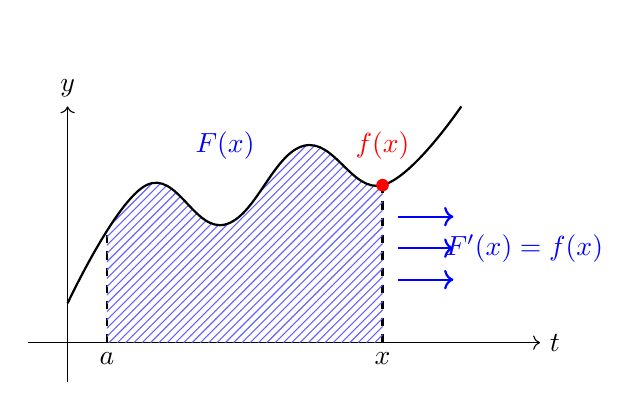
\begin{tikzpicture}[scale=1]
        % Define axes
        \draw[->] (-0.5,0) -- (6,0) node[right] {$t$};
        \draw[->] (0,-0.5) -- (0,3) node[above] {$y$};
        
        % Draw vertical lines for a and x (renamed from c and b)
        \draw[thick, dashed] (0.5,0) node[below] {$a$} -- (0.5,1.4);
        \draw[thick, dashed] (4,0) node[below] {$x$} -- (4,2);
        
        % Blue pattern only
        \begin{scope}
          \clip (0.5,-0.5) rectangle (4,4);
          \fill[pattern=north east lines, pattern color=blue!60] 
              plot[smooth, tension=0.7] coordinates {(0,0.5) (1,2) (2,1.5) (3,2.5) (4,2) (5,3)} 
              -- (5,0) -- (0.5,0) -- cycle;
        \end{scope}
        
        % Draw the function curve on top of everything
        \draw[thick] 
            plot[smooth, tension=0.7] coordinates {(0,0.5) (1,2) (2,1.5) (3,2.5) (4,2) (5,3)};
        
        % Draw 3 blue arrows vertically stacked to the right of the blue pattern
        \draw[->, blue, thick] (4.5-0.3,0.8) -- (5.2-0.3,0.8);
        \draw[->, blue, thick] (4.5-0.3,1.2) -- (5.2-0.3,1.2);
        \draw[->, blue, thick] (4.5-0.3,1.6) -- (5.2-0.3,1.6);
        
        % Add a red point at (4,2) and label it with f(x)
        \fill[red] (4,2) circle (0.08);
        \node[above, red] at (4,2.2) {$f(x)$};
        
        % Add label F'(x) = f(x) to the right of the blue arrows
        \node[blue] at (5.8,1.2) {$F'(x) = f(x)$};
        
        % Add F(x) label above the curve
        \node[blue] at (2,2.5) {$F(x)$};
      \end{tikzpicture}
      \caption{This theorem amazingly tells us that the rate at which the integral $F$ is increasing at $x$ (represented by the increasing area under the curve of $f$) is equal to the value of $f$ at the point $x$ itself! } 
      \label{fig:ftc1-illustration}
    \end{figure}
  \end{theorem}
  \begin{proof} 
    Listed. 
    \begin{enumerate}
      \item Since $f \in \mathcal{R}([a, b])$, let $M = \sup_{x \in [a, b]} |f(x)| < + \infty$. WLOG let $x, y \in [a, b]$ with $x < y$. Then, we can use the ``trick'' by writing the difference of $F$ as an integral, which follows from linearity of the integral over an interval. So, we have 
      \begin{align}
        |F(x) - F(y)| = \bigg| \int_x^y f(t) \, dt \bigg| & \leq \int_x^y |f(t)| \,dt \\
                                                          & \leq \int_x^y M \,dt  = M |y - x|
      \end{align}
      So given $\epsilon > 0$, we can take $\delta = \epsilon/M$ and $F$ is continuous. 

      \item Now let's claim 
        \begin{equation}
          \lim_{h \to 0} \frac{1}{h} \big( F(x_0 + h) - F(x_0) - f(x_0) h \big) = 0 \iff F^\prime (x_0) = f(x_0)
        \end{equation} 
        since if the limit exists, we can add $f(x_0)$ to both sides. The term in the limit is 
        \begin{equation}
          \frac{1}{h} \bigg| \int_a^{x_0 + h} f(t) \,dt - \int_a^{x_0} f(t) \,dt - f(x_0) h \bigg| \leq \frac{1}{h} \bigg| \int_{x_0}^{x_0 + h} f(t) \,dt - h f(x_0) \bigg|
        \end{equation}
        Now we do a trick that is simple but powerful. Notice that $h f(x_0) = \int_{x_0}^{x_0 + h} f(x_0) \,dt$, so we can join it with the integral.\footnote{Elgindi talked about how simple tricks can go a long way, e.g. the guy who was a master of Cauchy-Schwarz inequality.} So, 
        \begin{align}
          '' & = \frac{1}{h} \bigg| \int_{x_0}^{x_0 + h} f(t) - f(x_0) \,dt \bigg| \\ 
             & \leq \frac{1}{h} \int_{x_0}^{x_0 + h} \big| f(t) - f(x_0) \big| \,dt \\ 
             & \leq \frac{1}{h} \int_{x_0}^{x_0 + h} \sup_{t \in [x_0, x_0 + h]} \big| f(t) - f(x_0) \big| \,dt 
        \end{align} 
        Note that the supremum term in the integral is just a number, so evaluating it and taking the limit as $h \to 0$ gives 
        \begin{equation}
          \sup_{t \in [x_0, x_0 + h]} |f(t) - f(x_0)| \to 0 \text{ as } h \to 0
        \end{equation}
        since $f$ is continuous at $x_0$. 
    \end{enumerate}
  \end{proof}

  \begin{corollary}
    Every bounded function $f: [a, b] \longrightarrow \mathbb{R}$ on the closed interval $[a, b]$ and has only a finite number of points of discontinuity has a primitive, and every primitive of $f$ on $[a, b]$ has the form 
    \[\mathcal{F}(x) \coloneqq \int_a^x f(t)\,dt + c\]
    where $c$ is a constant. 
  \end{corollary}

  \begin{theorem}[Second Fundamental Theorem of Calculus]
    Let $f$ be a real-valued function on a closed interval $[a, b]$ with $\mathcal{F}$ any primitive of $f$ on $[a, b]$. If $f$ is Riemann-integrable (i.e. $f$ bounded with finite points of Lebesgue measure zero) on $[a, b]$, then 
    \begin{equation}
      \int_a^b f(x)\,dx  = \mathcal{F} \big|_a^b \equiv \mathcal{F}(b) - \mathcal{F}(a)
    \end{equation}

    \begin{figure}[H]
      \centering 
      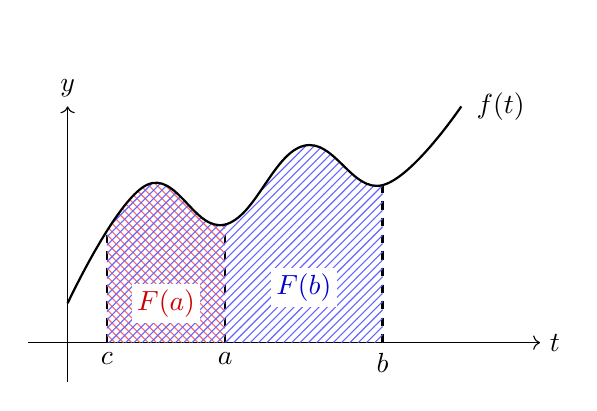
\begin{tikzpicture}[scale=1]
        % Define axes
        \draw[->] (-0.5,0) -- (6,0) node[right] {$t$};
        \draw[->] (0,-0.5) -- (0,3) node[above] {$y$};
        
        % Draw vertical lines for c, a, and b
        \draw[thick, dashed] (0.5,0) node[below] {$c$} -- (0.5,1.4);
        \draw[thick, dashed] (2,0) node[below] {$a$} -- (2,1.5);
        \draw[thick, dashed] (4,0) node[below] {$b$} -- (4,2);
        
        % Add borders to make areas clearer - using exact same coordinates as function
        \begin{scope}
          \clip (0.5,-0.5) rectangle (2,4);  % Clip to only show x from 0.5 to 5
          % Shade the area from c to a (F(a)) with red pattern
          \fill[pattern=north west lines, pattern color=red!60] 
              plot[smooth, tension=0.7] coordinates {(0,0.5) (1,2) (2,1.5) (3,2.5) (4,2) (5,3)} 
              -- (5,0) -- (0.5,0) -- cycle;
        \end{scope}

        \begin{scope}
          \clip (0.5,-0.5) rectangle (4,4);  % Clip to only show x from 0.5 to 5
          % Shade the area from c to a (F(a)) with red pattern
          \fill[pattern=north east lines, pattern color=blue!60] 
              plot[smooth, tension=0.7] coordinates {(0,0.5) (1,2) (2,1.5) (3,2.5) (4,2) (5,3)} 
              -- (5,0) -- (0.5,0) -- cycle;
        \end{scope}
        
        % Draw the function curve on top of everything
        \draw[thick] 
            plot[smooth, tension=0.7] coordinates {(0,0.5) (1,2) (2,1.5) (3,2.5) (4,2) (5,3)};
        
        % Label the curve
        \node[font=\bfseries] at (5.5,3) {$f(t)$};
        
        % Add labels for the areas with background
        \node[fill=white, text=red!80!black, font=\bfseries, inner sep=2pt] at (1.25,0.5) {$F(a)$};
        \node[fill=white, text=blue!80!black, font=\bfseries, inner sep=2pt] at (3,0.7) {$F(b)$};
      \end{tikzpicture}
      \caption{Graphical illustration of the Fundamental Theorem of Calculus, showing how the definite integral equals the difference of antiderivative values.} 
      \label{fig:ftc2-illustration}
    \end{figure}
  \end{theorem}
  \begin{proof}
    We already know that a bounded function on a closed interval having a finite number of discontinuities is integrable, and by the corollary, we are guaranteed an existence of a primitive $\mathcal{F}(x)$ of the function $f$ on $[a, b]$ with the form 
    \begin{equation}
      \mathcal{F} (x) \equiv \int_a^x f(t)\,dt + c
    \end{equation}
    Setting $x = a$, we find that $c = \mathcal{F}(a)$, and so 
    \begin{equation}
      \mathcal{F}(x) \equiv \int_a^x f(t)\,dt + \mathcal{F}(a)
    \end{equation}
    Evaluating $\mathcal{F}$ at $x = b$ gives
    \begin{equation}
      \int_a^b f(t)\,dt = \mathcal{F}(b) - \mathcal{F}(a)
    \end{equation}
  \end{proof}

  Now a direct application of the fundamental theorem of calculus is the integration by parts. By the product rule of differentiation, we have
  \begin{equation}
    (u \cdot v)^\prime (x) = (u^\prime \cdot v)(x) + (u \cdot v^\prime) (x)
  \end{equation}
  where by hypothesis, $u^\prime \cdot v, u \cdot v^\prime$ are continuous and hence integrable on $[a, b]$. Using the linearity of the integral and the 2nd fundamental theorem of calculus, we get
  \begin{equation}
    (u \cdot v) (x) \big|^b_a = \int_a^b (u^\prime \cdot v)(x)\,dx + \int_a^b (u \cdot v^\prime) (x)\,dx
  \end{equation}

  \begin{theorem}[Integration by Parts]
    Suppose $F, G: [a, b] \to \mathbb{R}$ are differentiable, with $F^\prime = f, G^\prime = g \in \mathcal{R}([a, b])$. Then 
    \begin{equation}
      \int_a^b F(x) g(x) \,dx = F(x) G(x) \big|_a^b - \int_a^b f(x) G(x) \,dx 
    \end{equation}
  \end{theorem} 
  \begin{proof}
    
  \end{proof}

  \begin{theorem}[Integral Form of the Remainder]
    If $f: E \longrightarrow \mathbb{R}$ has continuous derivatives up to order $n$ on the closed interval $[a, x]$, then Taylor's formula holds
    \begin{equation}
      f(x) = f(a) + \frac{f^\prime (a)}{1!} (x - a) + \ldots + \frac{f^{(n-1)}(a)}{(n-1)!} (x - a)^{n-1} + r_{n-1}(a; x)
    \end{equation}
    where 
    \begin{equation}
      r_{n-1} (a;x) = \frac{1}{(n-1)!} \int_a^x f^{(n)} (t) (x - t)^{n-1} \,dt
    \end{equation}
    This form is called \textbf{Taylor's formula with the integral form of the remainder}. 
  \end{theorem}
  \begin{proof}
    Using the 2nd fundamental theorem and the definite integration by parts formula, we can carry out the following chain of transformations, assuming continuity and differentiability when needed. 
    \begin{align*}
      f(x) - f(a) & = \int_a^x f^\prime (t) \,dt \\
      & = - \int_a^x f^\prime(t) (x - t)^\prime \,dt \\
      & = -f^\prime (t) (x - t)\big|_a^x + \int_a^x f^{\prime\prime} (t) (x - t) \,dt \\
      & = f^\prime (a) (x - a) - \frac{1}{2} \int_a^x f^{\prime\prime} (t) \big( (x - t)^2\big)^\prime \,dt \\
      & = f^\prime (x - a) - \frac{1}{2} f^{\prime\prime} (t) (x - t)^2 \big|_a^x + \frac{1}{2} \int_a^x f^{\prime\prime\prime} (t) (x - t)^2\,dt \\
      & = f^\prime(a) (x - a) + \frac{1}{2} f^{\prime\prime} (a) (x - a)^2 - \frac{1}{2 \cdot 3} \int_a^x f^{\prime\prime\prime} (t) \big((x - t)^3\big)^\prime\,dt \\
      & = \ldots \\
      & = f^\prime (a) (x - a) + \ldots + \frac{1}{(n-1)!} f^{(n-1)} (a)(x - a)^{n-1} + r_{n-1}(a;x)
    \end{align*}
    where $r_{n-1}(a;x)$ is given by the integral formula mentioned. 
  \end{proof}

\subsection{Integration over Paths and Rectifiable Curves}

  \begin{definition}[Integration For Vector Valued Functions]
    A function $f: [a, b] \to R^d$ is Riemann integrable if $f = (f_1, \ldots, f_d)$ and each component $f_i: [a, b] \to \mathbb{R}$ is in $\mathcal{R}([a, b])$. The integral is defined 
    \begin{equation}
      \int_a^b f(x) \,dx = \bigg(\int_a^b f_1, \ldots, \int_a^b f_d \bigg)
    \end{equation}
  \end{definition}

  Now since the codomain is $\mathbb{R}^d$, we can use the Euclidean norm $|v| \coloneqq \big( \sum_i v_i^2 \big)^{1/2}$ on it. 

  \begin{theorem}
    If $f \in \mathcal{R}([a, b], \mathbb{R}^d)$, then $|f| \in \mathcal{R}([a, b], \mathbb{R}^d)$ and 
    \begin{equation}
      \bigg| \int f \bigg| \leq \int |f|
    \end{equation}
  \end{theorem}
  \begin{proof}
    If $f \in \mathcal{R}([a, b], \mathbb{R}^d)$, then $f_i \in \mathcal{R}([a, b])$, and so 
    \begin{equation}
      |f| = \sqrt{f_1^2 + \ldots f_d^2} \in \mathcal{R}
    \end{equation}
    since $x \mapsto x^2$ and $x \mapsto \sqrt{x}$ are continuous. Now consider the vector $v = \int_a^b f$. Then 
    \begin{align}
      |v| = \bigg| \int_a^b f \bigg| \implies |v|^2 = \sum_{j=1}^d v_j^2 & = \sum_{j=1}^d v_j \int_a^b f_j \\ 
                                                                         & = \int_a^b \sum_{j=1}^d v_j f_j \\ 
                                                                         & = \int_a^b \sum_{j=1}^d v_j f_j \\
                                                                         & = \int_a^b \langle v, f(t) \langle \,dt \\ 
                                                                         & \leq  \int_a^b |v|\, |f(t)| \,dt
    \end{align}
    and so 
    \begin{equation}
      |v|^2 \leq |v| \cdot \int_a^b |f(t)| \,dt \implies |v| \leq \int_a^b |f(t)| \,dt 
    \end{equation}
  \end{proof}

  \begin{definition}[Curve]
    A \textbf{curve} is a function $\gamma: [0, 1] \to \mathbb{R}^d$. 
    \begin{enumerate}
      \item If $\gamma(0) = \gamma(1)$, then it is a \textbf{closed curve}. 
      \item If $\gamma$ is injective, then it is called a \textbf{simple curve}. 
    \end{enumerate}
  \end{definition}

  Curves are usually continuous but does not have to be. 

  \begin{example}
    The curve can have different parameterizations and/or image. For example, the two are different curves with the image in $S^1 \subset \mathbb{R}^2$. 
    \begin{align}
      \gamma(t) & = (\cos(2 \pi t), \sin(2 \pi t)) \\ 
      \Tilde{\gamma}(t) & = (\cos(4 \pi t), \sin(4 \pi t))
    \end{align} 
  \end{example}

  \begin{definition}[Length of a Curve]
    Given a curve $\gamma: [0, 1] \to \mathbb{R}^d$ and partition $P$ of $[0, 1]$, let 
    \begin{equation}
      \Lambda(\gamma, P) = \sum_{i=1}^N | \gamma(x_i) - \gamma(x_{i-1})| 
    \end{equation}
    i.e. the sum of the straight line distances between the curves. The \textbf{length} of the curve is defined as 
    \begin{equation}
      \Lambda(\gamma) \coloneqq \sup_P \Lambda(\gamma, P)
    \end{equation}
    If the length is finite, then we call this a \textbf{rectifiable curve}. 
  \end{definition}

  \begin{example}
    Consider the curve given by 
    \begin{equation}
      \gamma(t) = \bigg( t, t \sin \frac{1}{t} \bigg)
    \end{equation}
    $\gamma$ is continuous but $\gamma(t) < +\infty$. 
  \end{example}

  For most continuous curves, this is not finite, but there is a sufficient condition for it to be finite. 

  \begin{theorem}[$C^1$ Curves are Rectifiable]
    If $\gamma: [0, 1] \to \mathbb{R}^d$ is continuously differentiable, then $\gamma$ is rectifiable, and 
    \begin{equation}
      \Lambda(\gamma) = \int_0^1 |\gamma^\prime (t)| \,dt
    \end{equation}
  \end{theorem}
  \begin{proof}
    Since $\gamma^\prime (t)$ is continuous, then $|\gamma^\prime (t)|$ is continuous and $|\gamma^\prime (t)|$ is Riemann integrable. Now is $P$ is any partition of $[0, 1]$, then 
    \begin{align}
      \Lambda(x, P) = \sum_{i=1}^n |\gamma(t_i) - \gamma(t_{i-1})| & = \sum_{i=1}^n \bigg| \int_{t_{i-1}}^{t_i} \gamma^\prime (s) \,ds \bigg| \tag{Fund. Thm. of Calc.}\\ 
                                                                   & \leq \sum_{i=1}^n \int_{t_{i-1}}^{t_i} |\gamma^\prime (s)| \,ds \\ 
                                                                   & = \int_{t_0}^{t_n} |\gamma^\prime (s)| \,ds
    \end{align}
    So we've proved one inequality. Now we prove the other. Let $\epsilon > 0$ be given. Then since $\gamma^\prime (t)$ is continuous on compact $[0, 1]$, it must be uniformly continuous on $[0, 1]$. So $\exists \delta > 0$ s.t. 
    \begin{equation}
      |s - t| < \delta \implies |\gamma^\prime (s) - \gamma^\prime (t)| < \epsilon
    \end{equation} 
    Now take a partition $P$ of $[0, 1]$ s.t. $|t_i - t_{i-1}| < \delta$ for each $1 \leq i \leq N$. ...
  \end{proof}

  \begin{figure}[H]
    \centering 
    \includegraphics[scale=0.25]{img/Arc_Length_Integral.PNG}
    \caption{We can visualize this by partitioning the interval $[a, b]$ into the intervals $\Delta_i$, each with point $\xi_i \in \Delta_i$. This would partition the path to $\Gamma(\Delta_i)$, each with points $\Gamma(\xi_i)$, and at each point $\Gamma(\xi_i)$, we can imagine the velocity vector of the curve. By taking the magnitude of this vector $\Gamma^\prime (\xi_i)$, we multiply it by the length of the interval $\Delta x_i$ to get one rectangle, creating an approximation for one partition of the path. } 
    \label{fig:Arc_Length_Integral}
  \end{figure}

  \begin{corollary}[Length of the Graph of a $C^1$ Function]
    An immediate result of this formula is the formula for the length of a graph of a function $f: [a, b] \longrightarrow \mathbb{R}$ in $\mathbb{R}^2$, by looking at the paramaterization $t \mapsto (t, f(t)$. 
    \begin{equation}
      \Lambda(\gamma) = \int_a^b \sqrt{1 + (f^\prime (t))^2}\,dt
    \end{equation}
  \end{corollary}

  The question on the effect of paramaterization on the integral now arises. 

  \begin{definition}[Admissible Change of Parameter]
    The path $\Tilde{\Gamma}: [\alpha, \beta] \longrightarrow \mathbb{R}^3$ is obtained from $\Gamma: [a, b] \longrightarrow \mathbb{R}^3$ by an \textbf{admissible change of parameter} if there exists a smooth mapping 
    \[T: [\alpha, \beta] \longrightarrow [a, b]\]
    such that $T(\alpha) = a, T(\beta) = b$, $T^\prime (\tau) > 0$ (that is, the reparamaterization $T$ is monotonic) on $[\alpha, \beta]$, and 
    \[\Tilde{\Gamma} = \Gamma \circ T\]
    The series of mappings can be represented with the following commutative diagram, where $I_{\alpha, \beta} = [\alpha, \beta] \subset \mathbb{R}$ and $I_{a, b} = [a, b] \subset \mathbb{R}$. 
    \[
      \begin{tikzcd}
        I_{\alpha, \beta} \arrow{r}{T} \arrow{rd}{\Tilde{\Gamma}}& I_{a, b} \arrow{d}{\Gamma}\\
         & \mathbb{R}^3
      \end{tikzcd}
    \]

    \begin{figure}[H]
      \centering 
      \includegraphics[scale=0.25]{img/Admissible_Change_of_Parameter.jpg}
      \caption{Note that the points are labeled $0, 1, 2, 3, 4, 5$ do not represent numerical values, but rather the order in which the points are paramaterized. We can see from this ordering that $T$ is monotonic. } 
      \label{fig:Admissible_Change_of_Parameter}
    \end{figure}
  \end{definition}

  \begin{theorem}[Invariance of Arclength Integral under Admissible Change of Parameters]
    If a smooth path $\Tilde{\Gamma}: [\alpha, \beta] \longrightarrow \mathbb{R}^3$ is obtained from a smooth path $\Gamma: [a, b] \longrightarrow \mathbb{R}^3$ by an admissible change of parameter, then the lengths of the two paths are equal. That is, a
    \begin{equation}
      \int_a^b |\Gamma^\prime (t) |\,dt = \int_\alpha^\beta |\Tilde{\Gamma}^\prime (t)|\,dt \equiv \int_\alpha^\beta |(\Gamma \circ T)^\prime (t)|\,dt
    \end{equation}
  \end{theorem}

\subsection{Improper Integrals}

  Due to some limitations of the Riemann integral, we cannot integrate over "singularities" where either the interval or the function is unbounded. We develop the tools of improper integration to deal with this problem; there are two types of improper integrals. 

  \begin{definition}[Improper Integral of Unbounded Interval]
    Suppose the function $x \mapsto f(x)$ is defined on the interval $[a, +\infty)$ and is integrable on every closed interval $[a, b]$ contained in that interval. Then, we call the following term
    \[\int_a^{+\infty} f(x)\,dx \equiv \lim_{b \rightarrow + \infty} \int_a^b f(x)\,dx\]
    the \textbf{improper Riemann integral of $f$ over the interval $[a, +\infty)$} and 
    \[\int_{-\infty}^b f(x)\,dx \equiv \lim_{a \rightarrow -\infty} \int_a^b f(x)\,dx \]
    the \textbf{improper Riemann integral of $f$ over the interval $(-\infty, b]$}.If the limit exists, then we say that the integral \textbf{converges} and \textbf{diverges} otherwise. 
  \end{definition}

  \begin{definition}[Improper Integral of Unbounded Function]
    Suppose the function $x \mapsto f(x)$ is defined on the interval $[a, B)$ and integrable on any closed interval $[a, b] \subset [a, B)$. Then, we call the following term
    \[\int_a^B f(x)\,dx \equiv \lim_{b \rightarrow B^-} \int_a^b f(x)\,dx\]
    the \textbf{improper Riemann integral of $f$ over interval $[a, B)$} and
    \[\int_A^b f(x)\,dx \equiv \lim_{a \rightarrow A^+} \int_a^b f(x)\,dx\]
    the \textbf{improper Riemann integral of $f$ over interval $(A,b]$}.
  \end{definition}

  For cohesiveness, we can combine these two definitions of improper integrals into the following one. 

  \begin{definition}[Improper Integrals]
    Let $[a, \omega)$ be a finite or infinite interval and $x \mapsto f(x)$ a function defined on that interval and integrable over every closed interval $[a, b] \subset [a, \omega)$. Then, by definition
    \[\int_a^\omega f(x)\,dx \equiv \lim_{b \rightarrow \omega} \int_a^b f(x)\,dx\]
    if this limit exists as $b \rightarrow \omega, b \in [a, \omega)$. Similarly, given the finite or infinite interval $(\omega, b]$ with $f$ integrable over every closed interval $[a, b] \subset (\omega, b]$, we have
    \[\int_\omega^b f(x)\,dx \equiv \lim_{a \rightarrow \omega} \int_a^b f(x)\,dx\]
    Note that if $\omega \in \mathbb{R}$ and $f \in \mathcal{R}[a, \omega]$, the improper integral is equivalent to the regular Riemann integral. 
    \[\int_a^\omega f(x) = \lim_{b\rightarrow \omega} \int_a^b f(x)\,dx\]
  \end{definition}

  \begin{lemma}[Properties of the Improper Integral]
    Suppose $f, g$ are functions defined on interval $[a, \omega)$ (without loss of generality, we let $\omega$ be the upper limit of integration) and integrable on every closed interval $[a, b] \subset [a, \omega)$. Suppose the improper integrals 
    \[\int_a^\omega f(x)\,dx \text{ and } \int_a^\omega g(x)\,dx\]
    are well-defined. 
    \begin{enumerate}
      \item For any $\lambda_1, \lambda_2 \in \mathbb{R}$ the function $(\lambda_1 f + \lambda_2 g)(x)$ is integrable in the improper sense on $[a, \omega)$ and
      \[\int_a^\omega (\lambda_1 f + \lambda_2 g)(x)\,dx = \lambda_1 \int_a^\omega f(x)\,dx + \lambda_2 \int_a^\omega g(x)\,dx\]
      \item For any $c \in [a, \omega)$, 
      \[\int_a^\omega f(x)\,dx = \int_a^c f(x)\,dx + \int_c^\omega f(x)\,dx\]
      \item If $\varphi: [\alpha, \gamma) \longrightarrow [a, \omega)$ is a smooth strictly monotonic mapping with $\varphi(\alpha) = a$ and $\varphi(\beta) \rightarrow \omega$ as $\beta \rightarrow \gamma^-$, then the improper integral of the function $t \mapsto (f \circ \varphi)(t) \varphi^\prime (t)$ over $[\alpha, \gamma)$ exists and 
      \[\int_a^\omega f(x)\,dx = \int_\alpha^\gamma (f \circ \varphi)(t) \varphi^\prime (t)\,dt\]
    \end{enumerate}
  \end{lemma}

  Convergence of an Improper Integral

  Note that by definition, an improper integral 
  \[\int_a^\omega f(x)\,dx \equiv \lim_{b \rightarrow \omega} \int_a^b f(x) \,dx\]
  is a limit of the function 
  \[\mathcal{F}(b) \equiv \int_a^b f(x)\,dx\]
  as $b \rightarrow \omega$. This means that we can use the Cauchy criterion to determine the convergence of this limit, and hence, existence of this improper integral. 

  \begin{theorem}[Cauchy Criterion for Convergence of an Improper Integral]
  If the function $x \mapsto f(x)$ is defined on the interval $[a, \omega)$ and integrable on every closed interval $[a, b] \subset [a, \omega)$, then the integral 
  \[\int_a^\omega f(x)\,dx\]
  converges if and only if for every $\epsilon > 0$ there exists $B \in [a, \omega)$ such that the relation
  \[\Bigg| \int_{b_1}^{b_2} f(x)\,dx \bigg| < \epsilon\]
  holds for any $b_1, b_2 \in [a, \omega)$ satisfying $B < b_1$ and $B < b_2$. 
  \end{theorem}
  \begin{proof}
  We have
  \[\int_{b_1}^{b_2} f(x)\,dx = \int_a^{b_2} f(x)\,dx - \int_a^{b_1} f(x)\,dx = \mathcal{F}(b_2) - \mathcal{F}(b_1)\]
  and therefore the condition is simply the Cauchy criterion for the existence of a limit for the function $\mathcal{F}(b)$ as $b \rightarrow \omega$. 
  \end{proof}

  \begin{definition}[Absolute Convergence of an Improper Integral]
    The improper integral 
    \[\int_a^\omega f(x)\,dx\]
    \textbf{converges absolutely} if the integral
    \[\int_a^\omega |f|(x)\,dx\]
    converges. Clearly, the inequality
    \[\Bigg| \int_{b_1}^{b_2} f(x)\,dx \Bigg| \leq \Bigg| \int_{b_1}^{b_2} |f|(x)\,dx \Bigg|\]
    implies that if an improper integral converges absolutely, then it converges. 
  \end{definition}

  This study of absolute convergence reduces to the study of convergence of integrals of nonnegative functions. The following lemma is useful in determining convergence of such functions. 

  \begin{lemma}
    Let there be a function $f$ defined on interval $[a, \omega)$ that is also integrable over every closed interval $[a, b] \subset [a, \omega)$. If $f(x) \geq 0$ on $[a, \omega)$, then the improper integral 
    \[\int_a^\omega f(x)\,dx\]
    exists if and only if the function 
    \[\mathcal{F}(b) \equiv \int_a^b f(x)\,dx\]
    is bounded on $[a, \omega)$. 
  \end{lemma}
  \begin{proof}
  It is clear that 
  \[\int_a^\omega f(x)\,dx = \lim_{b \rightarrow \omega} \mathcal{F}(b)\]
  If $f(x)\geq 0$, then the function $\mathcal{F}(b)$ is nondecreasing on $[a, \omega)$ and therefore has a limit as $b \rightarrow \omega$ only if it is bounded (since every monotonically increasing sequence that is bounded always converges). 
  \end{proof}

  This leads to the familiar integral test for convergence of a series. 

  \begin{theorem}[Integral Test for Convergence of a Series]
  If the function $x \mapsto f(x)$ is defined on the interval $[1, +\infty)$, nonnegative, nonincreasing, and integrable on each closed interval $[1, b] \subset [1, +\infty)$, then the series 
  \[\sum_{n=1}^\infty f(n) = f(1) + f(2) + \ldots\]
  and the integral 
  \[\int_a^{+\infty} f(x)\,dx\]
  either both converge or both diverge. 
  \end{theorem}

  We can use the comparison test analogue to determine convergence of improper integrals. 

  \begin{theorem}[Comparison Test for Convergence of Improper Integrals]
  Suppose the functions $f(x), g(x)$ are defined on the interval $[a, \omega)$ and integrable on any closed interval $[a, b] \subset [a, \omega)$. If 
  \[0 \leq f(x) \leq g(x)\]
  on $[a, \omega)$, then 
  \[\int_a^\omega g(x)\,dx \text{ converges} \implies \int_a^\omega f(x)\,dx \text{ converges}\]
  and the inequality 
  \[\int_a^\omega f(x)\,dx \leq \int_a^\omega g(x)\,dx\]
  holds. Also, 
  \[\int_a^\omega f(x)\,dx \text{ diverges} \implies \int_a^\omega g(x)\,dx \text{ diverges}\]
  \end{theorem}

  Improper Integrals with Multiple Singularities

  \begin{definition}[Improper Integral with Both Limits as Singularities]
    Given singularities $\omega_1, \omega_2$, the improper integral is defined
    \[\int_{\omega_1}^{\omega_2} f(x)\,dx \equiv \int_{\omega_1}^c f(x)\,dx + \int_c^{\omega_2} f(x)\,dx\]
    where $c$ is an arbitrary point in $(\omega_1, \omega_2)$. 
  \end{definition}

  \begin{example}[Gaussian Integral]
  The integral 
  \[\int_{-\infty}^{+\infty} e^{-x^2}\,dx = \sqrt{\pi}\]
  \end{example}


\section{Surfaces}

  We can represent a $K$-dimensional subset $S \subset \mathbb{R}^N$ in multiple ways, where $K < N$. There are three conventional ways to do this. 
  \begin{enumerate}
      \item We can parameterize it with a function $f: D \subset \mathbb{R}^k \longrightarrow \mathbb{R}^n$ to create a \textbf{parameterized set} defined as the image of an \textit{injective} $f$ under $D$. Letting $\mathbf{x} \in \mathbb{R}^n$ and $\mathbf{u} \in \mathbb{R}^k$, the parameterization is defined 
      \[\mathbf{u} \mapsto f(\mathbf{u}) = \big( f_1 (\mathbf{u}), f_2 (\mathbf{u}), \ldots, f_n (\mathbf{u}) \big) \]
      
      \item A function $\mathbf{f}: \mathbb{R}^n \longrightarrow \mathbb{R}^m$ of the form $\mathbf{y} = \mathbf{f}(\mathbf{x})$ creates an \textbf{explicit representation} by defining all $(\mathbf{x}, \mathbf{y}) \in \mathbb{R}^{n+m}$ satisfying 
      \[\mathbf{y} = \mathbf{f}(\mathbf{x})\]
      
      \item A \textbf{level set} of the form $\mathbf{F}(\mathbf{x}) = \mathbf{0}$ creates an \textbf{implicit representation} by defining all $\mathbf{x} \in \mathbb{R}^n$ satisfying 
      \[\mathbf{F}(\mathbf{x}) = \mathbf{0}\]
      Now if $\mathbf{F}$ was scalar valued, then the equation $F(\mathbf{x}) = 0$ defines a hypersurface in $\mathbb{R}^n$ with codimension 1. If $\mathbf{F}$ is a $k$-vector valued function, then the implicit surface generally has codimension $k$, since we can interpret $\mathbf{F}(\mathbf{x}) = \mathbf{0}$ as a system of $k$ constraint equations. 
  \end{enumerate}
  Generally, the change of representations is simple only when the explicit representation $\mathbf{y} = \mathbf{f}(\mathbf{x})$ is given. The implicit form is $\mathbf{F}(\mathbf{x}, \mathbf{y}) = \mathbf{y} - \mathbf{f}(\mathbf{x}) = \mathbf{0}$, and the parameterized form is the map $\mathbf{x} \mapsto (\mathbf{x}, \mathbf{f}(\mathbf{x}))$. However, the explicit representation is very limited in usefulness, because it can only describe sets that are graphs of functions that pass the vertical line test. The implicit function theorem, stated later, states conditions under which an equation $\mathbf{F}(\mathbf{x}) = 0$ can be solved explicitly for any of the $x_i$'s. The other two representations are much more versatile, with the implicit representation being slightly more general, but the parametric form being more useful, since we can directly compute points on the $S$. Some examples are: 
  \begin{enumerate}
      \item a 1-dimensional path/curve in $\mathbb{R}^n$ 
      \item a 2-dimensional surface in $\mathbb{R}^3$ 
      \item a $k$-dimensional set in $\mathbb{R}^n$ 
  \end{enumerate}

  If these surfaces are smooth enough, then there must exist geometric tangent vectors, geometric tangent planes, and geometric orthogonal vectors on them. We say "geometric" to distinguish them from the vectors in the tangent space $T_{\mathbf{x}_0} \mathbb{R}^n$. It is important to know how to derive them. 

  \begin{theorem}[Explicit Representation]
  Let us have the surface $S \subset \mathbb{R}^{n+1}$ defined by $y = f(\mathbf{x})$ and a point on the surface $(\mathbf{x}_0, f(\mathbf{x}_0))$. 
  \begin{enumerate}
      \item To get the equation of the set of affine points forming the geometric tangent plane, we look at all points $(\mathbf{x}, y)$ satisfying 
      \[y = f(\mathbf{x}_0) + D f_{\mathbf{x}_0} (\mathbf{x} - \mathbf{x}_0)\]
      and to get an arbitrary tangent vector protruding from $\mathbf{x}_0$, we look at all vectors $(\mathbf{v}, w)$ of form 
      \[w = D f_{\mathbf{x}_0} \mathbf{v}\]
      i.e. all vectors of form $(\mathbf{v}, D f_{\mathbf{x}_0} \mathbf{v})$. 
      \item To get the equation of the orthogonal vector, convert this to the implicit representation $g(\mathbf{x}, y) = y - f(\mathbf{x}) = 0$, and see that the gradient is orthogonal to the tangent plane. So, the orthogonal vector at $\mathbf{x}_0$ is 
      \[\nabla g (\mathbf{x}_0, f(\mathbf{x}_0)) = \begin{pmatrix} - \nabla f(\mathbf{x}_0) \\ 1 \end{pmatrix}\]
      Note that indeed, dotting this with an arbitrary tangent vector of the form above gives 
      \[\begin{pmatrix} -\nabla f(\mathbf{x}_0) \\ 1 \end{pmatrix} \cdot \begin{pmatrix} \mathbf{v} \\ D f_{\mathbf{x}_0} \mathbf{v} \end{pmatrix} = - \nabla f(\mathbf{x}_0) \cdot \mathbf{v} + D f_{\mathbf{x}_0} \mathbf{v} = 0\]
  \end{enumerate}
  \end{theorem}

  Given a level set $S = \{ \mathbf{x} \in \mathbb{R}^n \mid f(\mathbf{x}) = c\}$, a vector $\mathbf{v}$ is a \textbf{tangent vector} of $S$ at $\mathbf{a}$ if the directional derivative (if it exists) satisfies
  \[\nabla_\mathbf{v} f (\mathbf{a}) = 0\]
  If $f$ is differentiable at $\mathbf{a}$, then this condition is equivalent to 
  \[D f_\mathbf{a} \mathbf{v} = 0\]
  Intuitively, $D f_\mathbf{a} \mathbf{v}$ answers the question: "If I move infinitesimally in the direction $\mathbf{v}$, what happens to $f$?" We would want this direction to preserve the value of $f = c$, and so the derivative should be $0$. Therefore, we look for the vectors $\mathbf{v}$ satisfying $D f_\mathbf{a} \mathbf{v} = 0$, i.e. the annihilator $(D f_\mathbf{a})^0 \subset \mathbb{R}^n$. This result is precisely the well-known theorem that states that "gradients are orthogonal to level sets." It is intuitive to claim that if we have some sort of directional vector $\mathbf{v}$, then this $\mathbf{v}$ must be "tangent" if the directional derivative towards $\mathbf{v}$ must be $0$, essentially staying within the level set of value $c$. 

  \begin{theorem}[Implicit Representation]
  Let us have the surface $S \subset \mathbb{R}^n$ defined by $F(\mathbf{x}) = 0$ and a point $\mathbf{a} \in S$. 
  \begin{enumerate}
      \item The gradient $\nabla F(\mathbf{x}_0)$ is simply the orthogonal vector at $\mathbf{x}_0$. 
      \item The set of all directional tangent vectors protruding from $\mathbf{x}_0$ is defined by the set of directional vectors $\mathbf{v}$ satisfying 
      \[\nabla F(\mathbf{x}_0) \cdot \mathbf{v} = 0\]
      and the set of all affine points forming the geometric tangent plane are all $\mathbf{x} \in \mathbb{R}^n$ satisfying 
      \[\nabla F(\mathbf{x}_0) \cdot (\mathbf{x} - \mathbf{x}_0) = 0\]
  \end{enumerate}
  \end{theorem}
  \begin{proof}
  This is trivial since we can invoke Reisz representation theorem and see that 
  \[D f_\mathbf{a} \mathbf{v} = 0 \implies \nabla_\mathbf{a} f \cdot \mathbf{v} = 0\]
  \end{proof}

  This theorem now simplifies our derivation of tangent planes of a function $f: \mathbb{R}^n \longrightarrow \mathbb{R}$. To find the equation of a tangent plane of $y = f(\mathbf{x})$ at $\mathbf{x} = \mathbf{a}$, we can simply write the one-line equation as 
  \[y = f(\mathbf{a}) + D f_{\mathbf{a}} (\mathbf{x} - \mathbf{x}_0)\]
  However, if we had an implicit function of the form $g(\mathbf{x}, y) = c$, then separating this into an explicit function of $y$ is hard. Therefore, we can simply treat $g$ itself as a function of the $n+1$ variables $(\mathbf{x}, y)$, and treat $g(\mathbf{x}, y) = c$ as a level set. 

  \begin{theorem}[Parametric Representation]
  Let us have $f: D \subset \mathbb{R}^k \longrightarrow \mathbb{R}^n$, with injective $f$ defining a surface $f(D) \subset \mathbb{R}^n$. Let us have $\mathbf{u}_0 \in D$ with $f(\mathbf{u}_0) = \mathbf{x}_0 \in f(D)$. Our idea is this: we compute $k$ directional derivatives of $f$ in $k$ linearly independent direction vectors at $\mathbf{u}_0$, which will give us $k$ (linearly independent, due to injectiveness of $f$, but not necessarily orthogonal) geometric tangent vectors protruding from $\mathbf{x}_0$ that span the tangent space $T_{\mathbf{x}_0}$. If $k = n-1$, then the orthogonal vector is uniquely defined to be the vector spanning $T_{\mathbf{x}_0}^\perp$, and is $k < n-1$, there is no unique orthogonal vector defined. 
  \begin{enumerate}
      \item The set of all directional tangent vectors $\mathbf{v}$ protruding from $\mathbf{x}_0$ is represented by the set of all linear combinations of the partials, aka the image of the Jacobian of $f$
      \[\{c_1 \partial_{u_1} f (\mathbf{u}_0) + \ldots + c_k \partial_{u_k} f (\mathbf{u}_0) \mid \mathbf{c} \in \mathbb{R}^n\} = \mathrm{Im} \begin{pmatrix} \vert & \ldots & \vert \\ \partial_{u_1} f (\mathbf{u}_0) & \ldots & \partial_{k} f (\mathbf{u}_0) \\ \vert & \ldots & \vert \end{pmatrix} = \mathrm{Im} D f_{\mathbf{u}_0}\]
      The tangent space is the space of all $\mathbf{x} \in \mathbb{R}^n$ of the form 
      \[f(\mathbf{x}_0) + D f_{\mathbf{x}_0} \mathbf{u} \text{ for all } \mathbf{u} \in \mathbb{R}^k\]
      \item If $k=n-1$, the orthogonal vector is the unique vector that is orthogonal to all $\partial_{u_i} f(\mathbf{u}_0)$, which can be computed using linear algebra techniques (e.g. kernel of $D f_{\mathbf{x}_0}$). If $n=3, k=2$, then this can simply be computed using the cross product. 
  \end{enumerate}
  \end{theorem}


\section{Integration of Forms}

\subsection{Line Integrals}

  \begin{definition}[Orientations, Simple Curves, Closed Curves]
  A path function $p: [a,b]\subset \mathbb{R} \longrightarrow \mathbb{R}^n$ determines a curve in $\mathbb{R}^n$ with endpoints $p(a)$ and $p(b)$. The direction the curve $p$ takes, that is from $p(a)$ to $p(b)$ in $\mathbb{R}^n$ is called the \textit{orientation} of $p$. A path or a curve with a defined orientation is called an \textit{oriented curve}. 

  A \textit{simple curve} $C$ to be the image of an injective piecewise $C^1$ map $c: I \subset \mathbb{R} \longrightarrow \mathbb{R}^3$. Since it is inejctive, it does not intersect itself, and $C$ is piecewise smooth in $\mathbb{R}^n$. If $I = [a,b]$, then $c(a)$ and $c(b)$ are the endpoints of the curve. A simple curve with an orientation is called an \textit{oriented simple curve}. 

  A closed curve $C$ is the image of piecewise $C^1$ map $c: [a,b] \longrightarrow \mathbb{R}^n$ such that $c(a) = c(b)$. That is, the endpoints of $C$ are equal. A \textit{simple closed curve} is a closed curve that is injective over the interval $[a,b)$. Note that a closed curve has two possible orientations. 
  \end{definition}

  If $C$ is an oriented simple curve or an oriented simple closed curve, then we can unambiguously define line integrals along them. 

  \begin{definition}
  Let $h$ be an injective function that takes $[\alpha,\beta] \subset \mathbb{R}$ to the interval $[a, b] \subset \mathbb{R}$. Given an oriented simple path function $p: [a,b]\subset \mathbb{R} \longrightarrow \mathbb{R}^n$, the composition
  \[\rho = p \circ h: [\alpha, \beta] \longrightarrow \mathbb{R}^n\]
  is called a \textit{reparamaterization} of $p$. Note that since $h$ is injective, it takes endpoints to endpoints. If $h$ preserves the direction in which the path travels, that is, if 
  \[(p \circ h)(\alpha) = a \text{ and } (p \circ h)(\beta) = b\]
  then $h$ is \textit{orientation preserving}. If
  \[(p \circ h)(\alpha) = b \text{ and } (p \circ h)(\beta) = a\]
  then $h$ is \textit{orientation reversing}. Note that a path $c$ having the same image as $p$ does not imply that $c$ is a reparamaterization of $p$, since $c$ may not be injective. 
  \begin{center}
      \includegraphics[scale=0.25]{img/Orientation_Preserving_Reversing.PNG}
  \end{center}
  \end{definition}

  \begin{definition}[Scalar Line Integral]
  Let $f: \mathbb{R}^n \longrightarrow \mathbb{R}$, which can be interpreted as a scalar field. Now define a $C^1$ path function 
  \[c: [a,b] \subset \mathbb{R} \longrightarrow \mathbb{R}^n \]
  such that the composition of functions
  \[f \circ c: [a, b] \subset \mathbb{R} \longrightarrow \mathbb{R}^n\]
  is continuous. Then, the \textit{path integral}, or \textit{scalar line integral}, of $f$ along the path $c$. is defined
  \begin{align*}
      \int_c f \;d s & = \int_a^b f\big(c(t)\big) ||c^\prime (t)|| \;d t \\
      & = \int_a^b f\big( x_1 (t), x_2 (t), ..., x_n (t)\big) ||c^\prime (t)|| \; d t
  \end{align*}
  If $c(t)$ is only piece-wise $C^1$, we can define the path integral by breaking $[a,b]$ into pieces over with $f\big( c(t)\big) ||c^\prime (t)||$ is continuous and then summing the integrals over the pieces. 
  That is, 
  \[\int_a^b f\big(c(t)\big) ||c^\prime (t)|| \;d t = \sum_{i = 0}^{n-1} \int_{\alpha_i}^{\alpha_{i+1}} f\big(c(t)\big) ||c^\prime (t)|| \; d t\]
  \end{definition}
  Note that since $f$ is a scalar-valued function, we can interpret a path integral as the sum of infinitesmal segments of the path $c$ having a weight determined by $f$ at each section. 
  If $f$ is a constant function outputting $1$ at every point, then the path integral just outputs the length of the path $c$ in $\mathbb{R}^n$. 
  \[L = \int_a^b f\big( c(t)\big) ||c^\prime (t)|| \; d t = \int_a^b ||c^\prime (t)|| \; d t\]

  \begin{definition}[Vector Line Integral]
  Let $F: \mathbb{R}^n \longrightarrow \mathbb{R}^n$ be a vector field on $\mathbb{R}^n$ that is continuous on the $C^1$ oriented path $c: [a, b] \subset \mathbb{R} \longrightarrow \mathbb{R}^n$. The \textit{line integral} of $F$ along $c$ is defined by the formula 
  \[\int_c F \cdot d s = \int_a^b F\big( c(t)\big) \cdot c^\prime (t) \; d t\]
  where $\cdot$ represents the dot product of $F$ with $c^\prime$ over the interval $[a,b]$. It is also commonly written in differential notation, 
  \[\int_c F \cdot ds = \int_c F \cdot (dx_1, \ldots, d x_n) = \int_c F_1 dx_1 + F_2 dx_2 + \ldots F_n dx_n\]
  \begin{center}
      \includegraphics[scale=0.27]{img/Vector_Line_Integral.PNG}
  \end{center}
   Similarly with path integrals, we can also define line integrals as the sum of integrals over piece-wise continuous sections of $c$. That is, given an oriented curve $C$ made up of several oriented component curves $C_i$, $i = 1, 2, ..., k$, we can paramaterize $C$ by paramaterizing the pieces $C_i$'s separately. Thus, we can treat $C = C_1 + ... C_k$ and get
  \[\int_C F \cdot d s = \sum_{i = 1}^k \int_{C_i} F \cdot d s\]
  Note that a vector line integral is a generalization of scalar line integrals, so any results holding for vector line integrals also holds for their scalar counterpart. 
  \end{definition}

  \begin{example}[Work]
  In mechanics, work $W$ is defined as 
  \[W = F \cdot d\]
  where $F$ is force and $d$ is displacement. With this knowledge, the reader can easily see that the work done by vector field $F$ on a particle traveling along a path $c$ from time $a$ to time $b$ can be calculated by the line integral
  \begin{align*}
      W & = \int_a^b F\big( c(t)\big) \cdot c^\prime (t) \; d t \\
      & = \int_c F_1 dx + F_2 dy + F_3 dz
  \end{align*}
  \end{example}

  \begin{theorem}[Invariance of Path Paramaterizations on Vector Line Integrals]
  Let $F$ be a vector field and $f$ be a scalar field, both continuous on the $C^1$ path function $p: [a,b] \longrightarrow \mathbb{R}^n$ and let $q: [\alpha, \beta] \longrightarrow \mathbb{R}^n$ be a reparamaterization of $p$. Then, 
  \begin{align*}
      q \text{ is orientation preserving} & \implies \int_p F \cdot d s = \int_q F \cdot d s \\
      q \text{ is orientation reversing} & \implies \int_p F \cdot d s = - \int_q F \cdot d s
  \end{align*}
  \end{theorem}

\subsection{Conservative Vector Fields}

  We now introduce a fundamental theorem about line integrals over gradient fields. Recall the fundamental theorem of calculus and it's equivalent form. 

  \begin{theorem}[Fundamental Theorem of Single Variable Calculus]
  Let function $\nabla g: \mathbb{R} \longrightarrow \mathbb{R}$ be the gradient of the single variable $C^1$ function $g: \mathbb{R} \longrightarrow \mathbb{R}$; that is, $\nabla g$ is a conservative vector field on $\mathbb{R}$. Then, 
  \[\int_a^b \nabla g (x) \,dx = g(b) - g(a)\]
  Note that in the single variable case, 
  \[\frac{d}{dx} g(x) = \nabla g(x)\]
  This means that the value of the integral of $\nabla g$ only depends on the value of $g$ at the endpoints of the interval $[a,b]$. 
  \end{theorem}

  We can extend this to line integrals for functions mapping $\mathbb{R}^n$ to $\mathbb{R}$. 

  \begin{theorem}[Invariance of Line Integrals in Conservative Vector Fields]
  Given that $F: \mathbb{R}^n \longrightarrow \mathbb{R}^n$ is a $C^1$ conservative vector field with $\nabla f = F$ for $C^2$ function $f: \mathbb{R}^n \longrightarrow \mathbb{R}$ and path function $p: [a,b] \longrightarrow \mathbb{R}^n$ is a piecewise $C^1$ path, then 
  \[\int_p F \cdot d s = \int_p \nabla f \cdot d s = f\big(p(b)\big) - f\big(p(a)\big)\]
  That is, the line integral of any path in a conservative vector field is dependent on the value of $f$ at the endpoints $p(a)$ and $p(b)$. 
  \begin{center}
      \includegraphics[scale=0.2]{img/Line_Integral_Independence_of_path.PNG}
  \end{center}
  \end{theorem}

  In physics, calculating the work done by a force represented by a vector field requires us to know the path that it travels through. 
  \[W = \int_p F \cdot ds\]
  However, in many cases $F$ is assumed to be conservative, so it is only necessary that we find the displacement of the particle from its endpoints, resulting in the simplification of the formula.  
  \[W = \int_p \nabla f \cdot ds = f\big( p(b)\big) - f \big(p(a)\big)\]

  \begin{corollary}[Equivalent Conditions for Vector Field to be Conservative]
  The following conditions are equivalent: 
  \begin{enumerate}
      \item $F: \mathbb{R}^n \longrightarrow \mathbb{R}^n$ is a conservative vector field. 
      \item The line integral of $F: \mathbb{R}^n \longrightarrow \mathbb{R}^n$ in curve $C$ is path independent; that is, if $C_1$ and $C_2$ are two paramaterizations of $C$, 
      \[\int_{C_1} F \cdot ds = \int_{C_2} F \cdot ds\]
      \item Given that $C$ is a closed loop, the line integral of $F: \mathbb{R}^n \longrightarrow \mathbb{R}^n$ across $C$ is $0$. 
      \[\oint_C F \cdot ds = 0\]
      \item The curl of $F: \mathbb{R}^3 \longrightarrow \mathbb{R}^3$ vanishes
      \[\curl{F} = \nabla \times F = \begin{pmatrix}
      \frac{\partial F}{\partial x} \\\frac{\partial F}{\partial y} \\\frac{\partial F}{\partial z} 
      \end{pmatrix} \times \begin{pmatrix}
      F_1\\F_2\\F_3
      \end{pmatrix}= 0\]
      \item The following partial derivatives of $F: \mathbb{R}^2 \longrightarrow \mathbb{R}^2$ are equal
      \[\frac{\partial F_1}{\partial y} = \frac{\partial F_2}{\partial x}\]
  \end{enumerate}
  \end{corollary}

  We can develop a bit of intuition to determine whether a vector field is conservative or not. If vector field $F$ is conservative, then there exists a smooth scalar field $f$ such that $\nabla f = F$. For each latitude and longitude on a certain map, we can give it an altitude as a function of those coordinates (picture a map with a bunch of hills and valleys). The gradient and thus the vector field is all the vectors that point in the direction of highest ascent. he vector field is all the vectors that point in the direction of highest ascent. Extending the metaphor the path integral is like starting on at a point and climbing the hills and valleys, creating work as you go up a hill (proportional to the steepness and thus the dot product of your motion vector with the gradient vector field in the path integral) and decreasing the work you put in by going down a hill. Since the path is closed, it is like you are going up and down the same amount overall, so the path integral is zero. Following this analogy, the vector field determined by this function (marked as arrows in the $x, y$ plane) is conservative. 
  \begin{center}
      \includegraphics[scale=0.28]{img/Conservative_Vector_Field.jpg}
  \end{center}
  If we can construct a closed loop around $F$ where the line integral is nonzero, then it means that we have ended up at a "higher" or "lower" (altitude) at the same point. This means that rather than being a certain landscape, there exist different "levels" of values at one point, like a spiraling staircase. For example, look at the solenoidal vector field below, where we can construct a closed loop (a circle going around the origin counterclockwise). There is no "surface" that can be defined such that it contains the solenoid. 
  \begin{center}
      \includegraphics[scale=0.28]{img/Solenoid_nonconservative.jpg}
  \end{center}
  Clearly, as a particle travels through the vector field along the path, it does positive work while it has zero displacement, and clearly, there exists no function that can output both these values as determined by vector field $F$. 

  \begin{theorem}[Helmholtz Decomposition]
  Let $F: \mathbb{R}^3 \longrightarrow \mathbb{R}^3$ be a $C^2$ vector field. Then, $F$ can be decomposed into a curl-free component and a divergence-free component. That is, there exists vector fields $A$ and $\Phi$
  \[F = - \nabla \cdot \Phi + \nabla \times A\]
  \end{theorem}

  \subsubsection{Curvature}
  \begin{definition}[Curvature at a Point]
  Let $c: [a, b] \longrightarrow C \subset \mathbb{R}^3$ be a unit-speed paramaterization of $C$, meaning that $||c^\prime (t)|| = 1$ for all $t \in [a,b]$, and let $p = c(t_0)$ be a point in $C$. The \textit{curvature} $\kappa(p)$ at $p$ is a mapping defined
  \[\kappa: C \longrightarrow \mathbb{R}, \;\; \kappa(p) \equiv ||c^{\prime \prime} (t_0)||\]
  Notice that since we require a unit speed paramaterization of $C$, we do not need to worry about how a given curve is paramaterized. 
  \end{definition}

  Since the curvature is defined pointwise for each point in curve $C$, we can integrate over all the curvatures in $C$ to define the total curvature. 

  \begin{definition}[Total Curvature]
  The \textit{total curvature} of a curve $c: [a,b] \longrightarrow C \subset \mathbb{R}^3$ is the scalar line integral 
  \[\int_C \kappa \, ds\]
  \end{definition}

  We now present an important theorem in differential geometry. 
  \begin{theorem}[Fary-Milnor Theorem]
  Given a unit speed paramaterization $c: [a,b] \longrightarrow C \subset \mathbb{R}^3$, if $C$ is closed (that is, $c(a)=c(b)$), then 
  \[\oint_C \kappa\, ds \geq 2 \pi\]
  and equals $2\pi$ only when $C$ is a circle. Furthermore, if $C$ is a closed space curve with 
  \[\oint_C \kappa\, ds \leq 4\pi\]
  then $C$ is "unknotted." That is, $C$ can be continuously deformed without every intersecting itself into a planar circle. Therefore, for knotted curves $C$, we have
  \[\oint_C \kappa \, ds > 4\pi\]
  \end{theorem}

\subsection{Surface Integrals}

  Surface integrals are the $2$-dimensional analogue, or the double integral version, of line integrals. It is the integration of surfaces. 

  \subsubsection{2-Dimensional Paramaterizations of Surfaces}
  Just like how we create path functions using a paramaterization function $p: [a, b] \subset \mathbb{R} \longrightarrow \mathbb{R}^n$, we can parameterize surfaces by defining a function 
  \[\varphi: D \subset \mathbb{R}^2 \longrightarrow \mathbb{R}^n, \;\;\; \varphi (u, v) \equiv \begin{pmatrix} x_1 (u, v) \\ \vdots \\ x_n (u, v) \end{pmatrix}\]
  The surface 
  \[S = \varphi(D)\]
  corresponding to the function $\varphi$ is its image. If $\varphi$ is differentiable or is of class $C^1$, then we call $S$ a \textit{differentiable} or $C^1$ surface, respectively. 

  For those that are familiar with differential geometry, this makes every paramaterized surface a 2-manifold induced by the single homeormophism $\varphi$. In fact, it is more than just locally homeomorphic; it is \textit{globally} homeomorphic. 


  \begin{definition}[Tangent Vectors of Surfaces Embedded in $\mathbb{R}^3$]
  Given surface paramaterization 
  \[\varphi: \mathbb{R}^2 \longrightarrow \mathbb{R}^3, \;\;\; \varphi(u, v) \equiv \begin{pmatrix}
  x (u, v) \\ y(u, v) \\ z(u, v) 
  \end{pmatrix}\]
  it is visually clear that there can be up to two linearly independent tangent vectors at a point on the surface $S$. We can calculate these two vectors by embedding two nonparallel paths in $D \subset \mathbb{R}^2$ and taking the derivative with respect to a point traveling through these paths, which would give us a tangent vector on $S$. To keep things simple, we take the partial derivatives with respect to $u$ and $v$. 
  \begin{center}
      \includegraphics[scale=0.28]{img/Partial_Derivatives_with_respect_to_U_V.PNG}
  \end{center}
  Clearly, these paths are functions 
  \begin{align*}
      \frac{\partial \varphi}{\partial u} \equiv \begin{pmatrix}
       \frac{\partial x}{\partial u} \\ \frac{\partial y}{\partial u} \\ \frac{\partial z}{\partial u}
      \end{pmatrix} : \mathbb{R}^2 \longrightarrow \mathbb{R}^3\\
      \frac{\partial \varphi}{\partial v} \equiv \begin{pmatrix}
       \frac{\partial x}{\partial v} \\ \frac{\partial y}{\partial v} \\ \frac{\partial z}{\partial v}
      \end{pmatrix} : \mathbb{R}^2 \longrightarrow \mathbb{R}^3
  \end{align*}
  where 
  \[\frac{\partial \varphi}{\partial u} (u_0 ,v_0), \; \frac{\partial \varphi}{\partial v} (u_0, v_0)\]
  represent two vectors in $\mathbb{R}^3$ that are tangent to $S$ at the point $\varphi(u_0, v_0) \in \mathbb{R}^3$. 
  \end{definition}

  We must make sure that the surface $S$ is smooth in the sense that (informally) there aren't any wrinkles, points, folds, or self-intersections in such a way that the tangent plane to the surface is not well-defined. 

  \begin{definition}[Regular Surfaces]
  To formalize this concept, we say that $S$ is \textit{regular}, or \textit{smooth}, at point $(u_0, v_0)$ if
  \[\frac{\partial \varphi}{\partial u} \times \frac{\partial \varphi}{\partial v} \neq 0\]
  where $\times$ is the Euclidean cross product. That is, if the vector that is orthogonal to the two tangent vectors is well defined at a point, the surface is said to be smooth at that point. Note that $\frac{\partial \varphi}{\partial u}$ is parallel to $\frac{\partial \varphi}{\partial v}$ if and only if their cross product is $0$. 
  \begin{center}
      \includegraphics[scale=0.3]{img/Cross_Product_Regular_Surfaces.PNG}
  \end{center}
  It is quite clear that $(\frac{\partial \varphi}{\partial u} \times \frac{\partial \varphi}{\partial v})(u_0, v_0) \neq 0 \implies \frac{\partial \varphi}{\partial u}$ and $\frac{\partial \varphi}{\partial v}$ are linearly independent. This means that an entire span of tangent vectors, i.e. a tangent plane, of the surface $S$ at $\varphi(u_0, v_0)$ exists. 
  $S$ is said to be \textit{regular} if it is regular at all points $\varphi(u_0, v_0) \in S$. 
  \end{definition}

  In fact, the tangent plane at $\varphi(u_0, v_0)$ is the set of points 
  \[\{\varphi(u_0, v_0) + \frac{\partial \varphi}{\partial u} (u_0, v_0) c_1 + \frac{\partial \varphi}{\partial v} (u_0, v_0) c_2 \; | \; c_1, c_2 \in \mathbb{R} \}\]
  which is precisely the affine tangent plane spanned by $T_u$ and $T_v$. Note also that the vector $T_u \times T_v$, if nonzero, is normal to this plane, which leads to this equivalent definition. 

  \begin{definition}[Tangent Planes of Surfaces]
  Given a paramaterized surface $\varphi: D \subset \mathbb{R}^2 \longrightarrow \mathbb{R}^3$ that is regular at $\varphi(u_0, v_0)$, the tangent plane of the surface $S$ at $\varphi(u_0, v_0) = (x_0, y_0, z_0)$ is defined
  \[\{(x, y, z) \in \mathbb{R}^3 \;|\; (x-x_0, y-y_0, z-z_0) \cdot n = 0\}\]
  where $n = (\frac{\partial \varphi}{\partial u} \times \frac{\partial \varphi}{\partial v})(u_0, v_0)$. 
  \end{definition}

  We finally construct the concept of signed areas before defining surface integration. 
  We have all the tools we need to calculate surface areas, but remember that integration also covers the concept of \textit{signed areas}, which could be negative. In order to define this, we define the concept of orientation on surfaces. 

  \subsubsection{Orientation of Surfaces}

  \begin{definition}[Oriented Surfaces]
  An \textit{oriented surface} is a two-sided surface with one side specified as the \textit{outside/positive} side and the other side as the \textit{inside/negative} side. Note that an oriented surface is not guaranteed to have two sides (e.g. a Mobius strip). To ensure that there exist two sides, $S$ must be regular. 

  Surprisingly, a paramaterization does not have an intrinsic orientation. Rather, we determine the orientation ourselves by choosing a unit vector that generally points towards the outside of the surface $S$. Again, this choice is arbitrary, but it is customary to choose a vector that generally points "out." Either way, the orientation (unit) vector at every point $\varphi(u, v) \in S$, denoted as $n$, is 
  \[n\big(\varphi(u, v)\big) = \pm \frac{\frac{\partial \varphi}{\partial u} \times \frac{\partial \varphi}{\partial v}}{\big|\big|\frac{\partial \varphi}{\partial u} \times \frac{\partial \varphi}{\partial v}\big|\big|}\]
  which can be visually calculated using the right hand rule. 
  \begin{center}
      \includegraphics[scale=0.23]{img/Orientation_Unit_Vector.PNG}
  \end{center}
  \end{definition}

  \begin{definition}[Orientation Preserving, Reversing Paramaterizations]
  Given an oriented surface $S$ with its positive side determined by the direction of unit vector $n\big( \varphi(u,v)\big)$, the paramaterization $\varphi$ is said to be \textit{orientation preserving} if 
  \[n \big( \varphi(u, v)\big) = \frac{\frac{\partial \varphi}{\partial u} \times \frac{\partial \varphi}{\partial v}}{\big|\big|\frac{\partial \varphi}{\partial u} \times \frac{\partial \varphi}{\partial v}\big|\big|}\]
  and \textit{orientation reversing} if
  \[n \big( \varphi(u, v)\big) = - \frac{\frac{\partial \varphi}{\partial u} \times \frac{\partial \varphi}{\partial v}}{\big|\big|\frac{\partial \varphi}{\partial u} \times \frac{\partial \varphi}{\partial v}\big|\big|}\]
  \end{definition}

  So, to find whether a paramaterization is orientation preserving or reversing, it suffices to find the cross product $T_u \times T_v$ and see if it points in the same direction of the normal vector $n$ (which should have already been determined when deciding the orientation of $S$). 

  Given a paramaterization $\varphi$ and an un-oriented surface $S$, we can also just construct $\varphi$ to be orientation-preserving (or reversing) by \textit{defining} the normal vector $n$ to be 
  \[n\big( \varphi(u, v)\big) = \frac{\frac{\partial \varphi}{\partial u} \times \frac{\partial \varphi}{\partial v}}{\big|\big|\frac{\partial \varphi}{\partial u} \times \frac{\partial \varphi}{\partial v}\big|\big|} \;\; \bigg( \text{or } n\big( \varphi(u, v)\big) = - \frac{\frac{\partial \varphi}{\partial u} \times \frac{\partial \varphi}{\partial v}}{\big|\big|\frac{\partial \varphi}{\partial u} \times \frac{\partial \varphi}{\partial v}\big|\big|} \bigg)\]
  So rather than finding out whether a paramaterization $\varphi$ is orientation preserving or reversing by comparing $T_u \times T_v$ with $n$, we have defined $n$ in a way such that $\varphi$ must be orientation preserving (or reversing). We can utilize these tools of paramaterization to now define the surface integral. 

  \subsubsection{Scalar, Vector Surface Integrals}

  A physical interpretation of a scalar surface integral is the weighted surface area of a certain surface. 

  \begin{definition}[Scalar Surface Integrals]
  Let $f: \mathbb{R}^3 \longrightarrow \mathbb{R}$ be a $C^1$ scalar field defined on a paramaterized surface $S \subset \mathbb{R}^3$ with paramaterization $\varphi: D \subset \mathbb{R}^2 \longrightarrow \mathbb{R}^3$. That is, $\varphi(D) = S$. We define the integral $f$ over $S$ to be
  \begin{align*}
      \iint_S f \; dS & = \iint_S f(x, y, z) \; dS \\
      & = \iint_D f\big( \varphi(u, v)\big) \bigg|\bigg|\frac{\partial \varphi}{\partial u} \times \frac{\partial \varphi}{\partial v}\bigg|\bigg| \; du \,dv
  \end{align*}
  Note that this will require us to transform $f$, a function of $x, y, z$, into the function $f \circ \varphi$ of $u, v$. Additionally, if the paramaterization of the surface $S$ is not defined, then it one must be constructed. It is also clear that if $S$ is a union of surfaces $S_i$, then its surface integral is the sum of the surface integrals of the $S_i$'s. 
  \end{definition}

  Letting the scalar field $f$ be the constant field equal to $1$, the scalar surface integral measures the surface area of $S$. 
  \[A(S) = \iint_S \; dS = \iint_D \Big|\Big|\frac{\partial \varphi}{\partial u} \times \frac{\partial \varphi}{\partial v}\Big|\Big| \; du\, dv\]
  It is easy to see that the orientation of the paramaterization $\varphi$ does not affect scalar surface integrals, since the sign of the orientation gets nullified by the absolute value sign over $||\frac{\partial \varphi}{\partial u} \times \frac{\partial \varphi}{\partial v}||$. 

  Its physical interpretation is to measure the rate at which a fluid (determined by a vector field $F$) is crossing a given surface $S$. It also has many applications in electromagnetism. 

  \begin{definition}[Vector Surface Integrals]
  Let $F$ be a vector field defined on surface $S$, the image of a paramaterized surface $\varphi$. The \textit{surface integral} of $F$ over $S$ is defined below, which is equivalent to summing up the dot product of the vector field and the normal vector to the surface. 
  \begin{center}
      \includegraphics[scale=0.3]{img/Vector_Surface_Integral.jpg}
  \end{center}
  It can be calculated with the following formulas by converting it into a scalar surface integral where the scalar field is the value of the dot product of the vector field with the normal vectors of the surface. 
  \begin{align*}
      \iint_{S} F \cdot d S & = \iint_S (F \cdot n) \; dS \\
      & = \iint_D \Bigg( F\big( \varphi(u, v)\big) \cdot \frac{\frac{\partial \varphi}{\partial u} \times \frac{\partial \varphi}{\partial v}}{\Big|\Big|\frac{\partial \varphi}{\partial u} \times \frac{\partial \varphi}{\partial v} \Big|\Big|} \Bigg) \, \bigg|\bigg|\frac{\partial \varphi}{\partial u} \times \frac{\partial \varphi}{\partial v}\bigg|\bigg|\; du\,dv \\
      & = \iint_D F\big(\varphi(u, v)\big) \cdot \bigg( \frac{\partial \varphi}{\partial u} \times \frac{\partial \varphi}{\partial v}\bigg) \; du\,dv
  \end{align*}
  \end{definition}

  Since we are now talking about vector fields, the orientation of the paramaterization is now significant. Visually, if the orientation of the surface $S$ generally aligns with the vector field $F$, then the integral will be positive (since two vectors $\alpha, \beta$ generally pointing in the same direction implies that $\alpha \cdot \beta > 0$). The orientation of the paramaterization, which is dependent on $\frac{\partial \varphi}{\partial u} \times \frac{\partial \varphi}{\partial v}$, determines the direction of the normal vector $n$ (since it is defined to be $(\frac{\partial \varphi}{\partial u} \times \frac{\partial \varphi}{\partial v}) / \big|\big|\frac{\partial \varphi}{\partial u} \times \frac{\partial \varphi}{\partial v}\big|\big|$. Therefore, changing the orientation of $\varphi$ will reverse the direction of $n$, which will then reverse the sign of the integral since $n$ now points in the opposite direction of the vector field $F$ than it previously did (by reversing the sign of the dot products). This is formalized in the theorem below. 

  \begin{theorem}[Invariance of Surface Paramaterizations on Vector Surface Integrals]
  Let $S$ be an oriented surface and let $\varphi_1$ and $\varphi_2$ be two regular paramaterizations with $F$ a continuous vector field defined on $S$. Then, assuming $\varphi_1$ is orientation preserving, 
  \begin{align*}
      \varphi_2 \text{ is orientation preserving } & \implies \iint_{\varphi_1} F \cdot d S = \iint_{\varphi_2} F \cdot d S \\
      \varphi_2 \text{ is orientation reversing } & \implies - \iint_{\varphi_1} F \cdot d S = \iint_{\varphi_2} F \cdot d S 
  \end{align*}
  \end{theorem}

  \subsubsection{Surface Integrals over Graphs}
  Given that we have the graph of a function $g: \mathbb{R}^2 \longrightarrow \mathbb{R}$ rather than a general surface, we can paramaterize it simply as
  \[\varphi(u, v) \equiv \big(u, v, g(u, v) \big)\]
  \begin{center}
      \includegraphics[scale=0.25]{img/Paramaterize_Surfaces_as_Graphs.PNG}
  \end{center}
  This means that 
  \[\frac{\partial \varphi}{\partial u} \times \frac{\partial \varphi}{\partial v} = 
  \begin{pmatrix}
  -\frac{\partial g}{\partial u} \\ -\frac{\partial g}{\partial v} \\ 1
  \end{pmatrix} \implies \bigg|\bigg|\frac{\partial \varphi}{\partial u} \times \frac{\partial \varphi}{\partial v} \bigg|\bigg| = \sqrt{1 + \Big(\frac{\partial g}{\partial u}\Big)^2 + \Big( \frac{\partial g}{\partial v}\Big)^2}\]
  So we can simplify the equation for the surface area $S$ of the graph of $g$ over the region $D$ in the $x y$-plane, as 
  \begin{align*}
      A(S) & = \iint_S \; d S = \iint_D \bigg|\bigg|\frac{\partial \varphi}{\partial u} \times \frac{\partial \varphi}{\partial v} \bigg|\bigg| \; d A \\
      & = \iint_D \sqrt{1 + \Big(\frac{\partial g}{\partial u}\Big)^2 + \Big( \frac{\partial g}{\partial v}\Big)^2} \; d u \, d v
  \end{align*}
  With the same $g$, we can find the weighed surface area of $S$ over the scalar function $f: \mathbb{R}^3 \longrightarrow \mathbb{R}$ with the formula
  \[\iint_S f \; d S = \iint_D f\big(u, v, g(u, v)\big) \sqrt{1 + \Big(\frac{\partial g}{\partial u}\Big)^2 + \Big( \frac{\partial g}{\partial v}\Big)^2} \; d u \, d v\]
  Finally, with the same graph $g$, the surface integral over the vector field $F$ is
  \begin{align*}
      \iint_S F \cdot d S & = \iint_D F\big(\varphi(u, v)\big) \cdot \bigg( \frac{\partial \varphi}{\partial u} \times \frac{\partial \varphi}{\partial v}\bigg) \; d u \, d v \\
      & = \iint_D \bigg( F_1(u, v) \Big(- \frac{\partial g}{\partial u}\Big) + F_2 (u, v) \Big( - \frac{\partial g}{\partial v} \Big) + F_3 (u, v) \bigg) \; d u \, d v
  \end{align*}

\subsection{Integral Theorems}

  Recall the differential notation for writing line integrals. For 2 and 3 dimensions, it is written as
  \begin{align*}
      & \int_C F \cdot d s = \int_C F \cdot (d x, d y) = \int_C F_1 \, d x + F_2 \, d y \\
      & \int_C F \cdot d s = \int_C F \cdot (d x, d y, d z) = \int_C F_1 \, d x + F_2 \, d y + F_3 \, d z 
  \end{align*}
  \subsubsection{Green's Theorem}
  Green's Theorem gives the relationship between a line integral around a simple closed curve $C$ and a double integral over the plane region $D$ bounded by $C$. 

  \begin{theorem}[Green's Theorem in $\mathbb{R}^2$]
  Let there be a 2-dimensional $C^1$ vector field $F$ on $\mathbb{R}^2$ defined on a simple oriented closed piecewise-smooth curve $C$ and its bounded region $D \subset \mathbb{R}^2$ (that is, $C = \partial D$). Let the orientation of the path of $C$ be such that it is traveling \textit{counterclockwise}, i.e. a point traveling through $C$ would see the region $D$ to its \textit{left}, denoted as $C^+$ and the clockwise orientation as $C^-$.  Then, 
  \[\oint_{C^+} F_1 \, d x + F_2 \, d y = \iint_D \bigg( \frac{\partial F_2}{\partial x} - \frac{\partial F_1}{\partial y} \bigg) \; d x \, d y\]
  By reversing the orientation, it is clear that we have
  \[\oint_{C^-} F_1 \, d x + F_2 \, d y = - \iint_D \bigg( \frac{\partial F_2}{\partial x} - \frac{\partial F_1}{\partial y} \bigg) \; d x \, d y\]
  Note that this theorem is expressed in terms of the components of the vector field $F$. 
  \begin{center}
  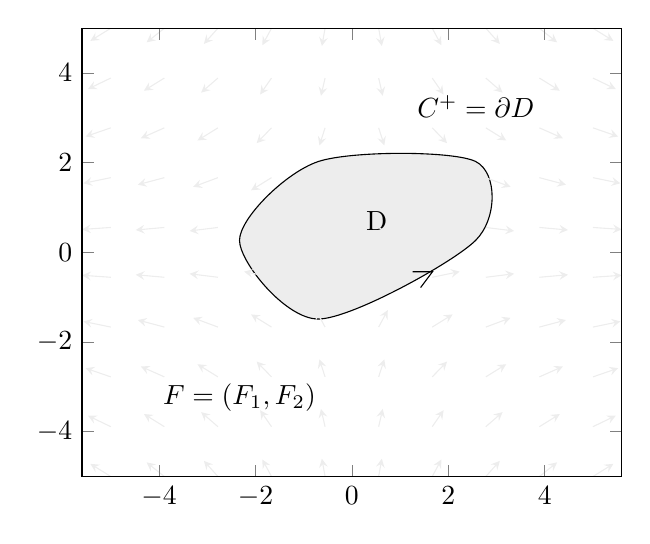
\begin{tikzpicture}
      \draw[fill=lightgray] plot [smooth cycle] coordinates {(2,3) (3,4) (5,4) (5,3) (3,2)};
      \node [above left] at (4,3) {D};
      \begin{axis}[view={0}{90}]
      \addplot3 [lightgray,-stealth,samples=10,
          quiver={
              u={3*x/pow(x^2 + y^2,1/2)},
              v={-2*y/pow(x^2 + y^2,1/2)},
              scale arrows=0.2,
          },] { 1};
      \end{axis}
      \node at (2,1) {$F = (F_1, F_2)$};
      \node at (5,4.7) {$C^+ = \partial D$};
      \draw (4.3,2.4)--(4.45,2.6)--(4.2,2.6);
  \end{tikzpicture}
  \end{center}
  \end{theorem}

  Green's theorem has many applications in physics. For example, in order to solve two-dimensional flow integrals measuring the sum of fluid outflowing from a volume, Green's theorem allows us to calculate the total outflow summed about an enclosing area . 

  \begin{corollary}
  Let $D$ be a region for which Green's theorem applies with positively oriented boundary $\partial D$. Then, the area of $D$ can be computed with the formula
  \[A(D) = \frac{1}{2} \oint_{\partial D} x \, d y - y \, d x\]
  \end{corollary}

  Green's theorem can be used to determine the area of centroid of plane figures solely by integrating over the perimeter. 

  \subsubsection{Stokes' Theorem}
  Green's theorem relates line integrals to double integrals. Stokes' theorem generalizes Green's theorem by relating line integrals to surface integrals of 2-dimensional surfaces embedded in $\mathbb{R}^3$. 

  \begin{theorem}[Stokes' Theorem]
  Let $S$ be an oriented regular surface defined by paramaterization $\varphi: D \subset \mathbb{R}^2 \longrightarrow \mathbb{R}^3$, and let the image of the boundary $\partial D$ under $\varphi$ be the boundary $\partial S$ of $S$. We can interpret $\partial S$ as a path mapping from $\mathbb{R} \longrightarrow S \subset \mathbb{R}^3$. 
  \begin{center}
    \includegraphics[scale=0.27]{img/Boundary_Mapping.PNG}
  \end{center}
  The orientation unit vector $n$ of $S$ induces the positive orientation of $\partial S$, denoted $\partial S^+$. Visually, if you are walking along the curve with your head is pointing in the same direction as the unit normal vectors while the surface is on the left then you are walking in the positive direction on $\partial S$. 
  \begin{center}
      \includegraphics[scale=0.8]{img/Stokes_Theorem_Orientation.png}
  \end{center}
  Given that $F$ is a $C^1$ vector field defined on $S$, then
  \[\iint_S \curl{F} \cdot dS = \iint_S \big( \nabla \times F \big) \cdot d S = \oint_{\partial S^+} F \cdot d s\]
  If $S$ has no boundary, that is, if the image of $p^\prime = \partial S$ is not a simple closed curve, then the integral is $0$. 
  \end{theorem}

  The above theorem implies that the vector surface integral of a surface without a boundary (i.e. a closed graph, such as a sphere) is always $0$ along the curl of any $C^1$ field. Geometrically, this means that given a closed solid $S$ with field $\nabla \times F$, the rate of flow of the vector field into $S$ is equal to the flow out of $S$. 

  \subsubsection{Gauss' Theorem}
  The divergence theorem relates the flux of a vector field through a closed surface to the divergence of the field in the volume enclosed. 

  \begin{theorem}[Gauss' Divergence Theorem]
  Let $V$ be a subset of $\mathbb{R}^3$. Denote by $\partial V$ the oriented closed surface that bounds $V$ (with outward pointing normal orientation vectors), and let $F$ be a $C^1$ vector field defined on a neighborhood of $V$. Then, 
  \[\iiint_V \Div{F} \; d V = \iiint_V (\nabla \cdot F) \; d V = \oiint_{\partial V} F \cdot d S = \oiint_{\partial V} (F \cdot n) \; dS\]
  where the two left-most integrals are volume integrals, and the two right-most integrals are surface integrals. Intuitively, this makes sense; the volume integrals represent the total of the sources in volume $V$, and the right hand side represents the total flow across the boundary $\partial V$. 
  \begin{center}
      \includegraphics[scale=0.35]{img/Gauss_Theorem_Volume.png}
  \end{center}
  \end{theorem}

\section{Sequences of Functions}

  Let us slightly extend the notion of limits of sequences with functions. 

  \begin{definition}[Pointwise Convergence]
    \label{def:pointwise-convergence}
    Let $E \subset \mathbb{R}$ and $f, f_n : E \to \mathbb{R}$. We say that $f_n \to f$ \textbf{pointwise} if 
    \begin{equation}
      \lim_{n \to \infty} f_n (x) = f(x) \text{ for all } x \in E
    \end{equation}
  \end{definition}

  The next question to ask is whether properties of functions are preserved under the limit operations. For example, if the $f_n$'s are continuous, differentiable, or Riemann integrable, is the same true for the limit function $f$? What are the relations between $f_n^\prime$ and $f^\prime$ or $\int f_n$ and $\int f$? To say that a function $f$ is continuous at a point $x$ means 
  \begin{equation}
    \lim_{t \to x} f(t) = f(x)
  \end{equation}
  For functions, the analogous result is whether 
  \begin{equation}
    \lim_{t \to x} \lim_{n \to \infty} f_n (t) = \lim_{n \to \infty} \lim_{t \to x} f_n (t)
  \end{equation}

  Is this true? Let's look at a few examples. 

  \begin{example}[Double Sequence May be Swappable]
    Consider the double sequence $\big( \frac{1}{m + n} \big)_{m, n \in \mathbb{N}}$. We can compute the limit as both $n, m \to +\infty$ in many ways. 
    \begin{enumerate}
      \item We can first set $m \to +\infty$, then $n \to +\infty$. 
      \item We can first set $n \to +\infty$, then $m \to +\infty$. 
      \item We might want to take $n$ twice as slow as $m$. 
    \end{enumerate}
    All of these converge to the same value of $0$, so there is no problem. 
  \end{example}

  \begin{example}
    Let $f_n (x) = x/n$. Then $f_n \to 0$ pointwise, where $0$ is the $0$ function. This is true since for every fixed $x$, we can set $n$ so large that $x/n < \epsilon$ for any $\epsilon$. 
  \end{example}

  In this case, we are considering a double sequence in $\mathbb{R}$. However, if we fix one value, then it becomes a sequence of functions, and we already have established that classes of functions form a vector space. In general, interchanging limits are not allowed. 

  \begin{example}[Cannot Exchange Limits Under Pointwise Convergence]
    Consider the slightly different sequence $\big( \frac{m}{m + n} \big)_{m, n}$. 
    \begin{enumerate}
      \item If $m >> n$, i.e. take the sequence of values $(10^k, k)$, then this will approach $1$. 
      \item If $n >> m$, i.e take the sequence of values $(k, 10^k)$, then this will approach $0$. 
      \item In intermediate cases, you can in fact get any number between $0$ and $1$. 
    \end{enumerate}
  \end{example}

  Therefore, in general, the limits are not equal. Even worse, the properties of these functions are violated. To get equality, we need to make a stronger assumption than simple existence of limits. 

  \begin{example}[Pointwise Limit of Continuous Functions is not Continuous]
    Let $f_n (x) : [0, 1] \to \mathbb{R}$  defined $f_n (x) = x^n$. Then, 
    \begin{align}
      0 \leq x < 1 & \implies x^n \to 0 \text{ as } n \to \infty \\ 
      x = 1 & \implies x^n \to 1 \text{ as } n \to \infty
    \end{align}
    So, 
    \begin{equation}
      f_n \to f^\ast (x) \coloneqq \begin{cases} 
        0 & \text{ if } x < 1 \\ 
        1 & \text{ if } x = 1
      \end{cases}
    \end{equation}
    Note that all $f_n$ are continuous but $f^\ast$ is discontinuous since 
    \begin{equation}
      \lim_{x \to 1} \lim_{n \to \infty} f_n (x) = 0 \neq 1 = \lim_{n \to \infty} \lim_{x \to 1} f_n (x)
    \end{equation}
  \end{example}

  \begin{example}[Pointwise Series Sum of Continuous Functions is not Continuous]
    Consider 
    \begin{equation}
      f_n (x) = \frac{x^2}{(1 + x^2)^n}
    \end{equation}
    and let 
    \begin{equation}
      f(x) = \sum_{n=0}^\infty f_n (x) = \sum_{n=0}^\infty \frac{x^2}{(1 + x^2)^n}
    \end{equation}
    Since $f_n (0) = 0$, we have $f(0) = 0$. For $x \neq 0$, the series is a convergent geometric series with sum $1 + x^2$. Therefore, 
    \begin{equation}
      f(x) = \begin{cases} 
        0 & \text{ if } x = 0 \\ 
        1 + x^2 & \text{ if } x \neq 0
      \end{cases}
    \end{equation}
    Therefore the sum of a convergent series of continuous functions may not be continuous. 
  \end{example}

  \begin{example}[Cannot Exchange Integrals and Limits Under Pointwise Convergence]
    Consider the function $f_n: [0, 1] \to \mathbb{R}$ defined by $f_n (0) = f_n (1/n) = 0$ and $f_n (1/2n) = 2n$, with everything else linearly interpolated. Then $f_n \to 0$ since it is constantly $0$ at $0$ and for every $x > 0$, there exists $1/N < x$ and so $f_n (x) = 0$ for all $n \geq N$. However, $\int_0^1 f_n (x) \,dx = 1$, so 
    \begin{equation}
      \lim_{n \to \infty} \int_0^1 f_n (x)\,dx \neq \int_0^1 \lim_{n \to \infty} f_n (x)\,dx
    \end{equation}
    So integration is not continuous with respect to the topology induced by pointwise convergence. 
  \end{example}

  The problem is not in the construction of the limits or the integral, but with the pointwise convergence. With pointwise convergence, 
  \begin{enumerate}
    \item we cannot exchange two limits, which implies limit of derivatives may not equal to the derivative of the limit
    \item limits do not preserve continuity 
    \item cannot exchange integrals and limits 
    \item cannot exchange sums
  \end{enumerate}

  \begin{example}
    Review. 
    \begin{equation}
      \bigg( 1 - \frac{1}{n} \bigg)^n \to e^{-1}
    \end{equation}
  \end{example}

  So now the motivation is to find properties of these sequences of functions that do allow these manipulations. 

\subsection{Uniform Convergence}

  The problem seems to be that certain points may converge at a much slower rate than others. Therefore, we want to impose some sort of uniform condition, which says that the values of the function at every point must converge. 

  \begin{definition}[Uniform Convergence]
    \label{def:uniform-convergence}
    Given $f_n : E \to \mathbb{R}$ of bounded functions, $(f_n)$ is said to \textbf{converge uniformly} to a bounded function $f: E \to \mathbb{R}$ if $\forall \epsilon > 0$, there exists $N \in \mathbb{N}$ s.t. 
    \begin{equation}
      n \geq N \implies |f_n (x) - f(x) | < \epsilon \text{ for all } x \in E
    \end{equation}
    the ``for all $x \in E$'' is the uniform part, which is similar to uniform continuity. 
  \end{definition}

  \begin{theorem}[Uniform Convergence iff Supremum of Difference Converges to 0]
    This is an immediate consequence of the definition. 
    \begin{equation}
      f_n \to f \text{ uniformly on } E \iff \lim_{n \to \infty} \sup_{x \in E} |f_n (x) - f(x)| = 0
    \end{equation}
  \end{theorem}
  \begin{proof}
    We can prove this with a bunch of iff statements. Let $f_n \to f$ uniformly, then this is equivalent to $\forall \epsilon > 0$, $\exists N \in \mathbb{N}$ s.t. $n \geq N$ implies
    \begin{align}
      & |f_n (x) - f(n)| < \epsilon \quad \forall x \in E \\ 
      & \iff M_n \sup_{x \in E} |f_n (x) - f(x)| \leq \epsilon \\ 
      & \iff M_n \to 0 \text{ as } n \to 0
    \end{align}
    which implies that $M_n \to 0$ as $n \to 0$. 
  \end{proof}

  Generally, to prove uniform convergence, you will need to find that $|f_n (x) - f(x)|$ is bounded by something that is independent of $x$, and it goes to $0$ as $n \to \infty$. Here is an equivalent condition. 

  \begin{definition}[Uniformly Cauchy]
    A sequence $f_n: E \to \mathbb{R}$ is called \textbf{uniformly Cauchy} if $\forall \epsilon > 0$, there exists $N \in \mathbb{N}$ s.t. $\forall n, m \geq N$, 
    \begin{equation}
      |f_n (x) - f_m (x)| < \epsilon \text{ for all } x \in E
    \end{equation}
  \end{definition}

  \begin{lemma}[Cauchy Criterion of Uniform Convergence]
    $(f_n)$ converges uniformly iff $(f_n)$ is uniformly Cauchy. 
  \end{lemma}
  \begin{proof}
    We prove bidirectionally. 
    \begin{enumerate}
      \item $(\rightarrow)$. Suppose $(f_n)$ converges uniformly on $E$, and let $f$ be the limit function. Then there exists $N \in \mathbb{N}$ s.t. 
      \begin{equation}
        n \geq N \implies |f_n (x) - f(x)| < \frac{\epsilon}{2} \text{ for all } x \in E
      \end{equation} 
      Therefore, 
      \begin{equation}
        n, m \geq N \implies |f_n (x) - f_m (x)| \leq |f_n (x) - f(x)| + |f(x) - f_m (x)| < \frac{\epsilon}{2} + \frac{\epsilon}{2} = \epsilon 
      \end{equation}
      for all $x \in E$. 

      \item $(\leftarrow)$. Suppose the uniform Cauchy criterion holds. For every $x \in E$, the sequence $(f_n (x))_n$ converges as a Cauchy sequence in $\mathbb{R}$. Call this limit $f(x)$. Thus the sequence $(f_n)$ converges pointwise to $f$. 

      Now let $\epsilon > 0$. Then, by uniform Cauchy, $\exists N \in \mathbb{N}$ s.t. 
      \begin{equation}
        n, m \geq N \implies |f_n (x) - f_m (x)| < \epsilon \quad \forall x \in E
      \end{equation}
      Now, if we fix $n$\footnote{This is a classic trick used to convert Cauchy convergence to regular convergence. What we want to do is that since given some $x_n$, the rest of the points $x_m$ must also be close to $x_n$, so the limit of the $x_m$ must also be close to $x_n$, which is basically the definition of convergence.}, we know that 
      \begin{equation}
        m \geq N \implies |f_n (x) - f_m (x)| < \epsilon 
      \end{equation}
      Now we can take the limit as $m \to \infty$, and therefore the limit of the LHS must be bounded by that of the RHS. 
      \begin{equation}
        \lim_{m \to \infty} |f_n (x) - f_m (x)| = |f_n (x) - f(x)| \leq \epsilon
      \end{equation}
      Now this is true for all $n \geq N$, which basically is the definition of convergence.\footnote{If you are dissatisfied with the $\leq$, just set $\epsilon/2$ to get strictly less than. }
    \end{enumerate}
  \end{proof}

  The wrong proof (that uniformly Cauchy implies uniform convergence) that I had in my first attempt was that I tried to directly bound the distances using some variant of the triangle inequality, like 
  \begin{equation}
    |f_n (x) - f_m (x)| \leq |f_n (x) - f(x)| + |f(x) - f_m (x)|
  \end{equation}
  However, this doesn't really help since this is an \textit{upper bound}. Perhaps we can use the reverse triangle inequality. 
  \begin{equation}
    | |f_n (x)| - |f_m (x)| | \leq |f_n (x) - f_m (x)|
  \end{equation}
  but again, this inequality lacks $f(x)$ entirely. 

  \begin{example}
    We have uniform convergence
    \begin{equation}
      \frac{\sin(e^n x)}{n} \to 0 \text{ since  } \bigg| \frac{\sin(e^n x)}{n} \bigg| \leq \frac{1}{n} \to 0
    \end{equation}
  \end{example}

  \begin{example}
    $f_n (x) = x^n$ does not converge uniformly to \textit{any} function in $[0, 1]$. It suffices to find a sequence $(y_n) \subset [0, 1]$ s.t. $|f_n (y_n) - f(y_n)| \not\to 0$ as $n \to \infty$. Take $y_n = 1 - \frac{1}{n}$. Then $f_n (y_n) \to \frac{1}{e} \neq 0$, but $f(y_n) \to 1$. 
  \end{example}

  \begin{example}
    The triangle functions do not converge uniformly since $f_n$ is unbounded, i.e. $f_n (\frac{1}{2n}) = 2n$, while $f_n ( \frac{1}{n}) = 0$. So we can construct two sequences that  
    \begin{equation}
      (1/2n) \to \infty, (1/n) \to 0 \text{ as } n \to \infty
    \end{equation}
  \end{example}

  \begin{lemma}[Uniform Convergence Implies Pointwise Convergence]
    Uniform convergence implies pointwise convergence. 
  \end{lemma}
  \begin{proof}
    Say $f_n \to f$ uniformly. Then for every $\epsilon > 0$, there exists a $N \in \mathbb{N}$ s.t. 
    \begin{equation}
      n \geq N \implies |f_n (x) - f(x)| < \epsilon \text{ for all } x \in E
    \end{equation}
    So just fix a point $x$, take any $\epsilon > 0$, and we have our $\delta$ due to uniform convergence. 
  \end{proof}

  \begin{theorem}[Weierstrass M-Test]
    Suppose $(f_n)$ is a sequence of functions on $E$, and suppose 
    \begin{equation}
      |f_n (x)| \leq M_n \text{ for all } x \in E
    \end{equation}
    for each $n \in \mathbb{N}$. Then if $\sum_n M_n$ converges, $\sum_n f_n$ converges uniformly.  
  \end{theorem}
  \begin{proof}
    If $\sum_n M_n$ converges, then for arbitrary $\epsilon > 0$, we have 
    \begin{equation}
      \bigg| \sum_{i=n}^m f_i (x) \bigg| \leq \sum_{i = n}^m M_n \leq \epsilon
    \end{equation}
    provided $n, m \in \mathbb{N}$ are large enough. Therefore this is uniformly Cauchy, and so uniformly convergent. 
  \end{proof} 

  Here is my wrong first attempt for a proof. Assume that $\sum_{k=1}^\infty M_k$ converges, and we wish to show that $\forall \epsilon > 0$, $\exists N \in \mathbb{N}$ s.t. 
  \begin{equation}
    n \geq N \implies \bigg| \underbrace{\sum_{k=1}^\infty f_k (x) - \sum_{k=1}^n f_k (x)}_{\text{not allowed}} \bigg| = \bigg| \sum_{k=n+1}^\infty f_k (x) \bigg|< \epsilon 
  \end{equation}
  The problem is that in our statement, we are assuming that we can actually subtract a finite term $\sum_{k=1}^n f_k (x)$ from a potentially divergent one: $\sum_{k=1}^\infty f_k(x)$. Therefore, we are assuming that this is convergent in the first place! This is exactly why we want to work with Cauchy sequences, which doesn't carry this kind of assumption, and so the sum from $i=n$ to $m$ is guaranteed to be finite. 

  After this, the rest of the steps are fine, since I use the fact that absolutely convergent series are also convergent, and so 
  \begin{equation}
    \bigg| \sum_{k=n+1}^\infty f_k (x) \bigg| \leq \sum_{k=n+1}^\infty |f_k (x)| \leq \sum_{k=n+1}^\infty M_k
  \end{equation}

  \begin{example}[Converse of Weierstrass M-test Not True]
    The converse is clearly not true, since we can just take any uniformly convergent bounded sequence and set $M_n \to +\infty$ as $n \to \infty$. 
  \end{example}

  The final theorem is a significant one. So far, we uniform convergence to prove that the limit of some sequence satisfies some property. In here, it's sort of the opposite. 

  \begin{theorem}[Dini's Theorem]
    \label{thm:dini}
    Suppose $K$ is compact, and 
    \begin{enumerate}
      \item $(f_n)$ is a sequence of continuous functions on $K$. 
      \item $f_n \to f$ pointwise on $K$. 
      \item $f$ is continuous.\footnote{Note that the pointwise limit of continuous functions may not be continuous!}
      \item $f_n \leq f_{n+1}$ for all $n \in \mathbb{N}$. 
    \end{enumerate}
    Then $f_n \to f$ uniformly on $K$. 
  \end{theorem} 
  \begin{proof}
    For convenience, let's define $g_n \coloneqq f - f_n \geq 0$, which is continuous on $K$. It suffices to prove that $g_n \to 0$ uniformly; that is, $\forall \epsilon > 0$, $\exists N \in \mathbb{N}$ s.t. 
    \begin{equation}
      n \geq N \implies |g_n (x)| < \epsilon
    \end{equation}
    Fix $\epsilon > 0$, and from compactness, we should already be thinking of trying to construct an open cover of $K$. Let 
    \begin{equation}
      E_n \coloneqq \{ x \in K \mid g_n (x) < \epsilon \}
    \end{equation}
    Note three things. 
    \begin{enumerate}
      \item First, $E_n$ is open as the preimage of continuous $g_n$. 
      \item Second $g_n$ is decreasing, so $g_n \geq g_{n+1}$, and so 
      \begin{equation}
        E_n \subset E_{n+1} \quad \forall n \in \mathbb{N}
      \end{equation}
      \item Third, $g_n \to 0$ pointwise, so at some point the $E_n$'s must cover all of $K$.\footnote{Remember that this is for \textit{fixed} $\epsilon$! This final point is not true if $\epsilon$ is not fixed.} 
      \begin{equation}
        \bigcup_{n = 1}^{\infty} E_n = K
      \end{equation}
    \end{enumerate}
    We have constructed an open cover, and now we take the fact that $K$ is compact to get a finite subcover $\{E_{n_k}\}_{k}$. But since the $E_n$'s are nested, we can set $N = \max_k \{n_k\}$, which implies $E_N = K$. Therefore, as long as $n \geq N$, $g_n$ is small enough so that it will map all of $E_N = K$ to a value less than $\epsilon$. We have 
    \begin{equation}
      n \geq N \implies g_n (x) = |g_n (x)| < \epsilon
    \end{equation}
  \end{proof}

  Let's reflect on this proof and how we used the theorem's assumptions. First, monotonicity of $f_n$ was needed to make sure that $E_n$ was increasing. Second, compactness of $K$ was needed to extract a finite subcover that we can exploit. 

\subsection{Limits of Uniformly Convergent Functions} 

  Now we will formalize and prove the manipulations that are unlocked by uniform convergence. 

  \begin{theorem}[Limits are Swappable]
    Suppose $f_n \to f$ uniformly over a set $E$ of a metric space. Let $x \in E^\prime$, and suppose that $\lim_{t \to x} f_n (t) = A_n$ for all $n$. Then, 
    \begin{enumerate}
      \item $(A_n)$ converges, and 
      \item we have 
        \begin{equation}
          \lim_{t \to x} f(t) = \lim_{n \to \infty} A_n \iff \lim_{t \to x} \lim_{n \to \infty} f_n (t) = \lim_{n \to \infty} \lim_{t \to x} f_n (t)
        \end{equation}
    \end{enumerate}
  \end{theorem}
  \begin{proof}
    Let $\epsilon > 0$, then by uniform continuity, there exists a $N \in \mathbb{N}$ s.t. 
    \begin{equation}
      n, m \geq N \implies |f_n (t) - f_m (t)| < \epsilon
    \end{equation}
    Now let $t \to x$, and since the limit exists, we have 
    \begin{equation}
      n, m \geq N \implies |A_n - A_m| < \epsilon
    \end{equation} 
    and so $(A_n)$ is by definition a Cauchy sequence in $\mathbb{R}$. Say that $A_n \to A$. 

    Now we wish to prove that $\lim_{t \to x} f(t) = A$. Take $\epsilon > 0$, and we wish to show that there exists some $\delta > 0$ s.t. 
    \begin{equation}
      |t - x| < \delta \implies |f(t) - A| < \epsilon
    \end{equation}
    Note that by the triangle inequality
    \begin{equation}
      |f(t) - A| \leq |f(t) - f_n (t)| + |f_n (t) - A_n| + |A_n - A|
    \end{equation}
    Therefore, we can take $\frac{\epsilon}{3} > 0$. 
    \begin{enumerate}
      \item By uniform convergence of $f_n \to f$, there exists a $N_1 \in \mathbb{N}$ s.t. 
      \begin{equation}
        n \geq N_1 \implies |f_n (x) - f(x)| < \frac{\epsilon}{3} \text{ for all } x \in E
      \end{equation}

      \item By convergence of $A_n \to A$, there exists a $N_2 \in \mathbb{N}$ s.t. 
      \begin{equation}
        n \geq N_2 \implies |A_n - A| < \frac{\epsilon}{3} 
      \end{equation}

      \item Therefore, choose $N = \max\{N_1, N_2\}$, and for this $N$, by convergence of $f_n (t) \to A_n$ we can choose a $\delta$ s.t. 
        \begin{equation}
          |x - t| < \delta \implies |f_n (t) - A_n| < \frac{\epsilon}{3} 
        \end{equation}
    \end{enumerate}
    This essentially bounds the three values, and so by choosing the $\delta$ in (3), we get 
    \begin{equation}
      |t - x| < \delta \implies |f(t) - A| \leq \frac{\epsilon}{3} + \frac{\epsilon}{3} + \frac{\epsilon}{3} = \epsilon
    \end{equation}
  \end{proof}

  \begin{corollary}[Uniform Limits of Continuous Functions are Continuous]
    If $(f_n)$ is a sequence of continuous functions on $E$, and if $f_n \to f$ uniformly on $E$, then $f$ is continuous on $E$. 
  \end{corollary}
  \begin{proof}
    Using the sequential definition of continuity, we claim that $\lim_{t \to x} f(t) = f(x)$. We know from the previous theorem that 
    \begin{equation}
      \lim_{t \to x} \underbrace{\lim_{n \to \infty} f_n (t)}_{= f(t)} = \lim_{n \to \infty} \underbrace{\lim_{t \to x} f_n (t)}_{= f_n (x)}
    \end{equation}
    where the LHS follows from $(f_n)$ being uniformly convergent, which implies pointwise convergence, and the RHS follows from $f_n$ being continuous.  
  \end{proof} 

  However, the converse is not true. A sequence of continuous functions may converge to a continuous function though not uniformly. Now let's move onto integration. 

  \begin{theorem}[Limits of Integrals are Integrals of Uniform Limits]
    Let $(f_n)$ be a sequence of Riemann integrable functions on $[a, b]$. If $f_n \to f$ uniformly on $[a, b]$, then $f \in \mathcal{R}([a, b])$ and 
    \begin{equation}
      \lim_{n \to \infty} \int_a^b f_n(x) \,dx = \int_a^b f(x) \,dx = \int_a^b \lim_{n \to \infty} f_n (x) \,dx 
    \end{equation}
  \end{theorem} 
  \begin{proof}
    Let $\epsilon_n = \sup | f_n (x) - f(x)|$ with the supremum taken over $a \leq x \leq b$. Then, 
    \begin{equation}
      f_n - \epsilon_n \leq f \leq f_n + \epsilon_n
    \end{equation}
    so the upper and lower integrals of $f$ satisfy 
    \begin{equation}
      \int_a^b (f_n - \epsilon_n) \,dx \leq \int_{\bar{a}}^b f(x) \,dx \leq \int_a^{\bar{b}} f(x) \,dx \leq \int_a^b (f_n + \epsilon_n) \,dx
    \end{equation}
    Hence, we have 
    \begin{equation}
      0 \leq \int_a^{\bar{b}} f(x)\,dx - \int_{\bar{a}}^b f(x) \,dx \leq 2 \epsilon_n (b - a) 
    \end{equation}
    and taking $n \to \infty$ sets $\epsilon_n \to 0$. 
  \end{proof}

  \begin{corollary}[Series Function May be Integrated Term by Term]
    If $f_n \in \mathcal{R}([a, b])$, and $f$ is defined 
    \begin{equation}
      f(x) \coloneqq \sum_{n=1}^\infty f_n (x) 
    \end{equation}
    with the series converging uniformly on $[a, b]$, then 
    \begin{equation}
      \int_a^b f(x) \,dx = \sum_{n=1}^\infty \int_a^b f_n (x)\,dx
    \end{equation}
  \end{corollary}

  Now we move onto differentiation. 

  \begin{theorem}[Limits of Derivatives]
    Suppose $(f_n)$ is a sequence of differentiable functions on $[a, b]$. If 
    \begin{enumerate}
      \item there exists some $x_0 \in [a, b]$ such that $(f_n (x_0))_n$ converges, and 
      \item $(f_n^\prime) \to f^\prime$\footnote{At this point, $f^\prime$ is just notation since $f$ isn't even defined.} on $[a, b]$, 
    \end{enumerate}
    Then $(f_n)$ converges uniformly to a function $f$, with 
    \begin{equation}
      f^\prime (x) = \lim_{n \to \infty} f_n^\prime (x) 
    \end{equation}
  \end{theorem} 
  \begin{proof}
    Choose $N \in \mathbb{N}$ s.t. for $n, m \geq N$, the following hold 
    \begin{equation}
      |f_n (x_0) - f_m (x_0)| < \frac{\epsilon}{2}, \qquad |f_n^\prime (t) - f_m^\prime (t)| < \frac{\epsilon}{2 (b - a)}
    \end{equation}
    which is possible due to convergence of $f_n (x_0)$ and uniform convergence of the derivative. Then applying the mean value theorem to the function $(f_n - f_m)$ gives 
    \begin{equation}
      |f_n (x) - f_m (x) - f_n (t) + f_m (t)| = (f_n - f_m)^\prime (c) |x - t| 
    \end{equation}
    for any $x, t \in [a, b]$ and $c \in (x, t)$. However, $(f_n - f_m)^\prime$ is bounded, so 
    \begin{equation}
      |f_n (x) - f_m (x) - f_n (t) + f_m (t)| \leq \frac{|x - t| \epsilon}{2 (b - a)} \leq \frac{\epsilon}{2}
    \end{equation}
    and therefore we can use the triangle inequality to get 
    \begin{align}
      |f_n (x) - f_m (x)| & \leq |f_n (x) - f_m (x) - f_n (x_0) + f_m (x_0)| + | f_n (x_0) - f_m (x_0)| \\
                          & \leq \frac{\epsilon}{2} + \frac{\epsilon}{2} = \epsilon
    \end{align}
    and so $f_n$ is uniformly Cauchy $\iff$ $(f_n)$ converges uniformly. 

    To show the equality of the limit, we fix a point $x \in [a, b]$ and define 
    \begin{equation}
      \phi_n (t) = \frac{f_n (t) - f_n (x)}{t - x}, \qquad \phi(t) = \frac{f(t) - f(x)}{t - x} 
    \end{equation}
    for $t \in (a, b), t \neq x$. Then, 
    \begin{equation}
      \lim_{t \to x} \phi_n (t) = f_n^\prime (x) 
    \end{equation}
    and we can see from the above inequality that 
    \begin{equation}
      | \phi_n (t) - \phi(t) | \leq \frac{\epsilon}{2 (b - a)}
    \end{equation}
    for $n, m \geq N$. So we can conclude 
    \begin{equation}
      \phi(t) = \lim_{n \to \infty} \phi_n (t)
    \end{equation}
  \end{proof}
  \begin{proof}
    Here is an alternative shorter proof of the equality (but not uniform convergence of $f_n$!) where we assume $f_n \in C^1([a, b])$. 
    Let's call the limit of $f^\prime_n$ to be $g$ to avoid confusion. We know that since $f_n^\prime$ is continuous, it's integrable and by the fundamental theorem of calculus we have 
    \begin{equation}
      f_n (x) - f_n (0) = \int_0^x f_n^\prime (t) \,dx 
    \end{equation}
    Since $f_n^\prime \to g$ uniformly and $f_n^\prime \in C^0$, $g$ is continuous and so we can define the function
    \begin{equation}
      f(x) \coloneqq f(0) + \int_0^x g(t) \,dt
    \end{equation}
    But we can see that by uniform convergence, we can swap integrals  
    \begin{align}
      f(x) - f(0) & = \int_0^x g(t) \,dt \\ 
                  & = \int_0^x \lim_{n \to \infty} f_n^\prime (t) \,dt \\
                  & = \lim_{n \to \infty} \int_0^x f_n^\prime (t) \,dt \\ 
                  & = \lim_{n \to \infty} f_n (x) - f_n (0) 
    \end{align}
    which implies that $f(x) - f(0) = \lim_{n \to \infty} f_n (x) - f_n (0)$ and so $f(x) = \lim_{n \to \infty} f_n (x)$. But since $f^\prime$ is continuous, the function $f$ defined above is differentiable, with derivative $f^\prime (x)$ to be whatever function is in the integral, i.e. $g(x)$. So
    \begin{equation}
      f^\prime (x) = g(x) = \lim_{n \to \infty} f_n^\prime (x)
    \end{equation}
  \end{proof}

\subsection{Equicontinuous Families} 

  Note that uniform convergence may not be met due to some counterexamples. In general, there are 3 ways that uniform convergence can fail to happen. 

  \begin{enumerate}
    \item \textit{Concentration}. Note that $x^n$ as $n \to \infty$ almost converges except at one point. 
    \item \textit{Translation}. Consider $f_n (x) = \sin(x - n)$. Then by increasing $n$ we are shifting it to $+\infty$. 
    \item \textit{Oscillation}. Consider $f_n (x) = \sin(nx)$. As $n$ increases the function oscillates widely. This is sort of like the worst.\footnote{It turns out that this is the same as (2) under the Fourier transform.} 
  \end{enumerate}

  We would like uniform convergence, so we want conditions to avoid lack of uniform convergence. Keep in mind to counterexamples. To avoid translation, work with compact space, or if not compact, have the functions decay uniformly. To avoid oscillation, we can bound the derivative, which is a restriction on each function $|f_n^\prime (x)| \leq M$. The Cauchy criterion is too much. To avoid going to infinity, just bound $f$: $|f_n (x)| \leq M$ for all $n \in \mathbb{N}, x \in X$. 

  The bounding of derivatives can be a bit strong. We aren't always working with differentiable functions, so we introduce a similar concept. 

  \begin{definition}[Equicontinuous Family]
    A family of functions $\mathcal{F}$ on $E$ is said to be \textbf{equicontinuous} if $\forall \epsilon > 0$ there exists a $\delta > 0$ s.t. 
    \begin{equation}
      |x - y| < \delta \implies |f(x) - f(y)| < \epsilon
    \end{equation}
    for all $x, y \in E, f \in \mathcal{F}$. 
  \end{definition}

  So this doesn't even depend on $f$. You can think of this as uniformly continuous for a class of functions that doesn't depend on $f$. The first class of equicontinuous functions you should know are those with bounded derivatives. 

  \begin{lemma}[Functions with Bounded Derivatives Are Equicontinuous]
    Fix $M \geq 0$. Then 
    \begin{equation}
      \mathcal{F}_n \coloneqq \{f : [0, 1] \to \mathbb{R} \mid |f^\prime (x)| \leq M \} 
    \end{equation}
    is an equicontinuous family. 
  \end{lemma}
  \begin{proof}
    For any $f \in \mathcal{F}$, the MVT $|f(x) - f(y)| = |f^\prime (c) (x - y)|$ for some $c \in (x, y)$. But since $f^\prime (c)$ is bounded by $M$, take $\delta = \epsilon/M$. 
  \end{proof}

  \begin{example}
    $\mathcal{F} = \{\sin(nx)\}_{n \in \mathbb{N}}$ is not equicontinuous on $[0, 1]$ since 
    \begin{equation}
      \bigg| \sin\Big( n \frac{\pi}{2n} \Big) - \sin \Big( n \frac{\pi}{n} \Big) \bigg| = 1
    \end{equation}
    for all $n$. So setting $x_n = \frac{\pi}{2n}, y_n = \frac{\pi}{n}$, we have $d(x_n, y_n) \to 0$ while $d(f(x_n), f(y_n)) \geq 1$. So this is not equicontinuous. 
  \end{example} 

  \begin{definition}[Pointwise Bounded]
    Given a sequence of functions $(f_n)$ over $E$, we say the sequence is \textbf{pointwise bounded} if it satisfies each of the equivalent conditions. 
    \begin{enumerate}
      \item There exists some function $\phi(x)$ s.t. $|f_n (x)| < \phi(x)$ for all $x \in E, n \in \mathbb{N}$. 
      \item For every $x \in E$, the sequence $(|f_n (x)|)_n$ is bounded. 
    \end{enumerate}
  \end{definition}

  \begin{definition}[Uniformly Bounded]
    Given a sequence of functions $(f_n)$ over $E$, we say the sequence is \textbf{uniformly bounded} if there exists some $M$ s.t. $|f_n (x)| \leq M$ for all $x \in E, n \in \mathbb{N}$. 
  \end{definition}

  Therefore, uniform boundedness is stronger, since this bound doesn't even depend on $x$. 

  \begin{lemma}[Uniform Boundedness Implies Pointwise Boundedness]
    Uniform boundedness implies pointwise boundedness. 
  \end{lemma}
  \begin{proof}
    Take $\phi(x) = M$. 
  \end{proof}

  We may wonder what the conditions are for the converse. The following theorem gives us those conditions. 

  \begin{theorem}[Conditions for Uniform Boundedness]
    If $K$ is compact, with 
    \begin{enumerate}
      \item $f_n$ is continuous on $K$ for each $n$
      \item $f_n$ pointwise bounded. 
      \item $f_n$ equicontinuous on $K$
    \end{enumerate}
    Then $\{f_n\}$ is uniformly bounded. 
  \end{theorem}
  \begin{proof}
    
  \end{proof}

  If $(f_n)$ is pointwise bounded on $E$ and $E_1$ is a countable subset of $E$, it is always possible to find a subsequence $(f_{n_k})$ that converges for every $x \in E_1$. As an intuitive example, suppose 
  \begin{enumerate}
    \item $(f_{2n} (q_1))$ converges 
    \item $(f_{3n} (q_2))$ converges 
    \item $(f_{5n} (q_3))$ converges 
    \item $(f_{7n} (q_4))$ converges 
  \end{enumerate}
  So combining the first two, we have that $(f_{6n}(q_i))$ converges for $i = 1, 2$. Continuing on, $(f_{30n} (q_i))$ converges for $i = 1, 2, 3$. But you can't do this infinitely. So if you want a single subsequence s.t. all the sequences converges, we can do 
  \begin{equation}
    f_2, f_6, f_{30}, f_{210}, f_{2310}, \ldots
  \end{equation}
  Since 
  \begin{enumerate}
    \item if you take out $f_2$, it is a subsequence of $(f_{3n})$ which converges for $q_2$, and 
    \item if you also take out $f_{6}$, it is a subsequence of $(f_{6n})$ which converges for $q_1, q_2$, and 
    \item if you also take out $f_{30}$, it is a subsequence of $(f_{30n})$ which converges for $q_1, q_2, q_3$
  \end{enumerate}
  so $f_{n_k} (q_i)$ converges for all $i$. Now let's formalize this argument. 

  \begin{lemma} 
    Let $(f_n)$ be a sequence of functions on $[0, 1]$ that's uniformly bounded. Let $\{q_m\}_{m=1}^\infty$ be a countable set of numbers in $[0, 1]$. Then $\exists$ a subsequence $(f_{n_k})$ for which $f_{n_k} (q_m)$ is convergent for all $m \in \mathbb{N}$. 
  \end{lemma}
  \begin{proof}
    Intuitively, if we find a sequence of functions, we want to look at each point---say $1$---and look at $(f_n (1))_n$. $(f_n (1))$ is bounded and so contains a convergent subsequence $(f_{n_k} (1))_k$. Now with this subsequence, we look at $(f_{n_k} (0))_k$ which is bounded and therefore $(f_{n_{k_j}}(0))_j$ converges, and $(f_{n_{k_{j}}}(1))_j$ must converge as a subsequence of convergent $(f_{n_k} (1))_k$. Now do this for all $q$'s, and we get a single subsequence that converges for all of them. 

    For ease of notation, let $f_{ij}$ denote the $j$th term of the $i$th subsequence. Then there exists $(f_{n, 1})_n$ s.t. $(f_{n, 1} (q_1))_n$ converges. Take a subsequence $f_{n, 2}$ of $f_{n, 1}$ s.t. $(f_{n, 2} (q_2))_n$ converges. Given $(f_{n, k})_n$, find a subsequence of it, called $(f_{n, k+1})_n$ for which $(f_{n, k+1} (q_{k+1}))_n$ converges. Now $(f_{n, n})_n$ is a subsequence of the original one ($n$th term of $n$th subsequence) for which $(f_{q, n})_n$ is eventually a subsequence of $(f_{n, j})_n$ for any fixed $j$. 
  \end{proof} 

  Now the Ascolli's theorem gives us conditions to get rid of translation, oscillations, and infinity. To prove the second statement, we will need a lemma, so we state it now, along with providing a neat trick for constructing sequences. 

  \begin{theorem}[Arzela-Ascolli's Theorem]
    We claim the following. 
    \begin{enumerate}
      \item If a sequence of continuous functions $f_n: [0, 1] \to \mathbb{R}$ (or more generally, over a compact set) converges uniformly, then they form an equicontinuous family. 
      \item If a sequence of functions $f_n: [0, 1] \to \mathbb{R}$ is equicontinuous and so uniformly bounded, then it has a uniformly convergent subsequence. 
    \end{enumerate}
  \end{theorem}
  \begin{proof}
    Assume $(f_n)$ is uniformly convergent. Then it is uniformly Cauchy. To prove equicontinuity, given a $\epsilon > 0$ we need to find a $\delta > 0$ for all the functions. Since $f_n$ is uniformly Cauchy, $\exists N$ s.t. if $n \geq N$, then 
    \begin{equation}
      \sup_{x \in [0, 1]} | f_n (x) - f_N (x) | < \epsilon/3
    \end{equation} 
    Consider the first $N$ functions $f_1, \ldots, f_N$. They are all continuous on a compact set and so uniformly continuous. So for each $f_i$, there exists a $\delta_i$ s.t. $|x - y| < \delta_i \implies |f_i (x) - f_i (y)| < \epsilon$. So take $\delta = \frac{1}{3} \min_i \delta_i > 0$. So for all $1 \leq i \leq N$, 
    \begin{equation}
      |x - y| < \delta \implies |f_i (x) - f_i (y)| < \epsilon/3
    \end{equation} 
    and for $n \geq N$, 
    \begin{equation}
      |f_n (x) - f_n (y)| \leq \underbrace{|f_n (x) - f_N (x)}_{< \epsilon/3} + \underbrace{f_N (x) - f_N (y)}_{< \epsilon/3} + \underbrace{f_N (y) - f_n (y)}_{< \epsilon/3} < \epsilon
    \end{equation} 
    For the second part, let $E = \mathbb{Q} \cap [0, 1]$. It is a good thing that $E$ is dense in $[0, 1]$. Let $(f_n)$ be an equicontinuous on $[0, 1]$ and uniformly bounded. Due to the lemma, there exists a $(f_{n_k})_k$ so that the $f_{n_k}$ converges pointwise on $E$ (since $E$ is countable). We will now use equicontinuity of $(f_{n_k})_k$ to prove it's uniformly Cauchy on $[0, 1]$, which will imply that it's convergent. To make notation easier we will call $f_{n_k} = g_k$. Let $\epsilon > 0$. Since $g_k$ is equicontinuous, $\exists \delta > 0$ s.t. 
    \begin{equation}
      |x - y| < \delta \implies |g_k (x) - g_k (y)| < \epsilon
    \end{equation} 
    Since $E = \{q_1, q_2, \ldots \}$ is dense in $[0, 1]$, $\{B_\delta (q_i) \}_{i=1}^\infty$ is an open cover of $[0, 1]$. Since $[0, 1]$ is compact, there exists a finite subcover 
    \begin{equation}
      [0, 1] \subset \bigcup_{j=1}^N B_{\delta} (q_{i_j})
    \end{equation}
    Since $(g_k (q_{i_j}))$ converges for each $1 \leq j \leq N$, there exists $M_j$ s.t. 
    \begin{equation}
      n, m \geq M_j \implies |g_n (q_{i_j} - g_m (q_{i_j}))| < \epsilon
    \end{equation}
    Take $M = \max_j M_j$. Now if $m, n \geq M$, given $x \in [0, 1]$ $\exists q_i$ with $1 \leq i \leq N$ so that $x \in B_\delta (q_i)$, and so 
    \begin{align}
      |g_n (x) - g_m (x)| & \leq \underbrace{| g_n (x) - g_n (q_i)|}_{< \epsilon} + \underbrace{| g_n (q_i) - g_m (q_i)|}_{< \epsilon} + \underbrace{|g_m (q_i) - g_m (x)|}_{< \epsilon} < 3\epsilon
    \end{align}
    where the first and third inequalities come from equicontinuity, and the middle come from convergence on $E$. So by setting $\delta/3$ we are done. 
  \end{proof}

  \begin{example}
    An important application is in the existence of minimizers/maximizers for optimization problems involving functions. To minimize 
    \begin{equation}
      J(f) = \int_0^1 \sqrt{1 + f^\prime (t)} \,dt 
    \end{equation}
    is the length of the curve of $f: [0, 1] \to \mathbb{R}$. To minimize the length of the curve, we must search over a set of functions. So to use EVT, you must know what the compact subsets of functions. 
  \end{example}

  Ascolli's theorem exactly characterizes these compact subsets. These compact subsets of function spaces is the closure of equicontinuous functions. 

  \begin{corollary}
    A set of functions $K \subset C([0, 1])$ is compact iff it is, under the supremum metric $\sup_{x \in [0, 1]}$, 
    \begin{enumerate}
      \item closed 
      \item bounded 
      \item equicontinuous
    \end{enumerate}
    The first two are needed for finite dimensions. The third condition is for function spaces. 
  \end{corollary} 

  \begin{theorem}[Contraction Mapping Theorem]
    Let $(X, d)$ be a metric space with $J: X \to X$ and let there exist $c < 1$ s.t.  
    \begin{equation}
      d(J(x), J(y)) \leq c d(x, y) \text{ for all } x, y \in X
    \end{equation}
    Then there exists a unique $x^\ast \in X$ s.t. $J(x^\ast) = x^\ast$. 
  \end{theorem}

\subsection{The Stone-Weierstrass Theorem} 

  The Stone-Weierstrass theorem is a bit more general, while the Weierstrass approximation theorem is for polynomials. 

  \begin{theorem}[Weierstrass Approximation Theorem]
    If $f \in C([a, b])$, there exists a sequence of polynomials $(p_n)$ that converges uniformly to $f$. 
  \end{theorem}

  \begin{lemma} 
    If $f: [0, 1] \to \mathbb{R}$ is continuously differentiable on $[0, 1]$, then 
    \begin{equation}
      \lim_{n \to \infty} \int_0^1 f(x) \sin(nx) \,dx = 0
    \end{equation} 
    This means that as $n \to \infty$, the integral becomes small. 
  \end{lemma}
  \begin{proof}
    
  \end{proof}

  Now we prove a stronger version. 

  \begin{theorem}
    For every $f \in C([0, 1])$, 
    \begin{equation}
      \lim_{n \to \infty} \int_0^1 f(x)\, \sin(nx) \,dx = 0
    \end{equation}
  \end{theorem}
  \begin{proof}
    Let $\epsilon > 0$. Then by the Weierstrass approximation theorem\footnote{aka, the set of polynomials is dense in the set of continuous functions with the supremum metric. Remember polynomial interpolation, which is for a finite number of points. This is a little different.}, there exists a polynomial $p: [0, 1] \to \mathbb{R}$ for which 
    \begin{equation}
      \sup_{x \in [0, 1]} | p(x) - f(x)| < \epsilon 
    \end{equation}
    Now consider 
    \begin{align}
      \bigg| \int_0^1 f(x) \, \sin(nx) \,dx \bigg| & \leq \bigg| \int_0^1 p(x) \sin(nx) \,dx \bigg| + \bigg| \int_0^1 (f(x) - p(x)) \sin(nx) \,dx \bigg| \\
                                                   & \leq \bigg| \int_0^1 p(x) \sin(nx) \,dx \bigg| + \epsilon \\
                                                   & \leq 2 \epsilon 
    \end{align}
    where the first inequality is the triangle inequality, the second is due to the Weierstrass approximation theorem, and the third is due to $p(x)$ being infinitely differentiable, and so by the lemma above it is $\leq \epsilon$. 

  \end{proof}

  \begin{theorem}
    
  \end{theorem}
  \begin{proof}
    Suppose for the sake of contradiction that $\sin(n_k x) \to g(x)$ uniformly for subsequence $(n_k)_k$. Then $g(x)$ must be continuous on $[0, 1]$. Then 
    \begin{equation} 
      \int_a^b g(x)^2 \,dx = \lim_{n \to \infty} \int_0^1 g(x) \sin(n_k x) \,dx = 0
    \end{equation}
    due to the theorem, which implies that $g = 0$. But since $g(nx) = \pm 1$ for some $x$ for all $n$, we have a contradiction. 
  \end{proof}

\subsection{Approximation of the Identity} 

  \begin{definition}[Approximation of the Identity]
    A family of functions $\{\varphi_\epsilon\}$ parameterized by $\epsilon$ is called an \textbf{approximation of the identity} if 
    \begin{enumerate}
      \item $\int_{-\infty}^{\infty} \varphi_\epsilon (y) \,dy = 1$ 
      \item $\lim_{\epsilon \to 0} \int_{|y| > \delta} \varphi_\epsilon (y) \,dy = 0$ for all $\delta > 0$ 
      \item $\varphi_\epsilon \geq 0$.\footnote{This condition is flexible, but it makes things a bit easier for now.}
    \end{enumerate}
  \end{definition}

  \begin{example}
    Consider the functions $f_\epsilon$ satisfying $f(-\epsilon) = f(\epsilon) = 0$, $f(0) = 1/\epsilon$, and everything in between linearly interpolated. Then this is an approximation of the identity. 
  \end{example}

  \begin{example}
    Take any $\varphi \geq 0$ s.t. $\int_{-\infty}^\infty \varphi = 1$ and define 
    \begin{equation}
      \varphi_\epsilon = \frac{1}{\epsilon} \varphi \bigg( \frac{x}{\epsilon} \bigg)
    \end{equation}
    which we can think of as squeezing the function horizontally to $0$ and making the amplitude very large. Then we see that 
    \begin{equation}
      \int_{-\infty}^{\infty} \varphi_\epsilon (y) \,dy = \int_{-\infty}^{\infty} \frac{1}{\epsilon} \varphi \bigg(\frac{y}{\epsilon} \bigg) = \int_{-\infty}^\infty \varphi(x) \,dx = 1
    \end{equation}
    Fix $\delta > 0$. Then 
    \begin{equation}
      \int_\delta^{\infty} \varphi_\epsilon (x) \,dx = \int_\delta^\infty \frac{1}{\epsilon} \varphi \bigg( \frac{x}{\epsilon} \bigg) \,dx = \int_{\delta/\epsilon}^\infty \varphi(y) \,dy \to 0 \text{ as } \epsilon \to 0
    \end{equation}
    Since $\delta$ is fixed, we have $\delta/\epsilon \to +\infty$ as $\epsilon \to 0$, and so this integral of the tail above converges to $0$.  
  \end{example} 

  The approximation of the identity (AoI) has an amazing property. 

  \begin{theorem}
    Let $\{\varphi_\epsilon\}$ be an AoI. Assume $f: \mathbb{R} \to \mathbb{R}$ is bounded and continuous. Then 
    \begin{equation}
      \lim_{\epsilon \to 0} \int_{-\infty}^\infty \varphi_\epsilon (y) \, f(y) \,dy = f(0)
    \end{equation}

    \begin{figure}[H]
      \centering 
      \caption{The triangle has area $1$. Now if you integrate the product of $\varphi_\epsilon (y)$ and $f(y)$, it's like taking the product and multiplying by $f$. But as $\epsilon \to 0$, the triangle's area is $1$, and at the end you just multiply by $f(0)$. } 
      \label{fig:aoi}
    \end{figure}
  \end{theorem}
  \begin{proof}
    We have 
    \begin{align}
      \bigg| \int_{-\infty}^\infty \varphi_\epsilon (y) \, f(y) \,dy - f(0) \bigg| & = \bigg| \int_{-\infty}^\infty \varphi_\epsilon (y) \, \big( f(y) - f(0) \big) \,dy \bigg| \\ 
                                                                                   & \leq \bigg| \int_{-\delta}^{\delta} \varphi_\epsilon (y) \big( f(y) - f(0) \big) \,dy \bigg| + \bigg| \int_{|y| > \delta} \varphi_\epsilon (y) \big( f(y) - f(0) \big) \,dy \bigg| \\ 
                                                                                   & \leq \sup_{y \in [-\delta, \delta]} |f(y) - f(0)| + 2 M \int_{|y| > \delta} \varphi_\epsilon (y) \,dy 
    \end{align}
    where the final step follows from the left integral is less than $\sup_{[-\delta, \delta]} |f(y) - f(0)|$, and for the right integral, we have $f(y) - f(0) \leq 2 \sup |f| \leq 2 M$. Since you don't know the limit exists, you take the limsup, 
    \begin{equation}
      \limsup_{\epsilon \to 0} \bigg| \int_{-\infty}^\infty \varphi_\epsilon (y) \, f(y) \,dy - f(0) \bigg| \leq \sup_{y \in [-\delta, \delta]} |f(y) - f(0)| \to 0 \text{ as } \delta \to 0
    \end{equation}
  \end{proof}

  \begin{corollary}[Convolution]
    If $\{f_\epsilon\}$ is an AoI with $f$ bounded and continuous and $x \in \mathbb{R}$, we have 
    \begin{equation}
      \lim_{\epsilon \to 0} \int_{-\infty}^\infty \varphi_\epsilon (y) \, f(x - y) \,dy  = f(x)
    \end{equation}
    This is called the \textbf{convolution} of $f$ with $\varphi_\epsilon$. 
  \end{corollary}

  \begin{definition}[Dirac Delta Function]
    $\varphi_\epsilon \to \delta_0$ as $\epsilon \to 0$, the Dirac delta function. This is a limit. 
  \end{definition}

  \begin{theorem}
    Consider the functions 
    \begin{equation}
      \varphi_n (x) = \begin{cases} 
        c_n (1 - x^2)^n & \text{ if } x \in [-1, 1] \\ 
        0 & \text{ else }
      \end{cases}, \qquad c_n = \bigg( \int_{-1}^1 (1 - x^2)^n \,dx \bigg)^{-1}
    \end{equation}
    Then, 
    \begin{equation}
      \int_{-1}^1 \varphi_n (x) = \int_{-\infty}^\infty \varphi_n (x) \,dx = 1
    \end{equation}
    so $\{\varphi_n\}$ is an approximation of the identity. 
  \end{theorem}
  \begin{proof}
    Note that $c_n$ is chosen such that $\int_{-\infty}^\infty \varphi_n (x) \,dx = 1$ and $\varphi_n \geq 0$. We want to show 
    \begin{equation}
      \int_{|x| > \delta} \varphi_n (x) \,dx \to 0 \text{ as } n \to \infty \text{ for all } \delta > 0
    \end{equation}
    We claim that $c_n \leq 10 \sqrt{n}$. since we wish to upper bound the multiplicative inverse of an integral, it suffices to lower bound the inverse---i.e. the integral itself. 
    \begin{align}
      \int_{-1}^1 (1 - x^2)^n \,dx = 2 \int_0^1 (1 - x^2)^n \,dx & \geq 2 \int_0^{1/\sqrt{n}} (1 - x^2)^n \,dx \\
                                                                 & \geq 2 \int_0^{1/\sqrt{n}} (1 - nx^2) \,dx 
    \end{align}
    where the last inequality follows from the binomial inequality $(1 - s)^n \geq 1 - sn$. Therefore, the final integral is now computable, so it equals 
    \begin{equation}
      '' = 2 \bigg(x - \frac{nx^3}{3}\bigg) \bigg|_0^{1/\sqrt{n}} = \frac{4}{3} \frac{1}{\sqrt{n}} \implies c_n \leq \bigg( \frac{4}{3} \frac{1}{\sqrt{n}})^{-1} < \sqrt{n}
    \end{equation}  
    Now we have 
    \begin{align}
      \int_{|x| > \delta} \varphi_n (x) \,dx & = 2 \int_\delta^{+\infty} \varphi_n (x) \,dx \\ 
                                             & = 2 \int_\delta^1 c_n (1 - x^2)^n \,dx \\ 
                                             & \leq 20 \sqrt{n} \int_\delta^1 (1 - x^2)^n \,dx \\ 
                                             & \leq 20 \sqrt{n} (1 - \delta^2)^n \to 0 \text{ as } n \to \infty 
    \end{align} 
    Note that we could have claim that the bound be $c_n \leq (10\sqrt{n})^{1000}$ and this would still be true. 
  \end{proof} 

  \begin{theorem}[Stone-Weierstrass Theorem]
    Let $f \in C([a, b])$. Then $\forall \epsilon > 0$, $\exists$ a polynomial $p$ s.t. 
    \begin{equation}
      d(f, p) \coloneqq \sup_{x \in [a, b]} d\big( f(x), p(x) ) < \epsilon
    \end{equation}
    This is equivalent to saying that $\mathbb{R}[x]$ is dense in $C([a, b])$, or that for any $f \in C([a, b])$, $\exists$ sequence $(p_n)$ of polynomials s.t. $p_n \to p$ uniformly on $[a, b]$. 
  \end{theorem}
  \begin{proof}
    By translation and dilation, it suffices to take $[a, b] = [-1, 1]$. This is because translation/dilations are automorphisms (?). It also suffices to consider only $f$ for which $f(-1) > 0$ and $f(1) = k$ for some number $k$. This is because we can always replace $f$ with $\Tilde{f}$ defined by 
    \begin{equation}
      \Tilde{f}(x) \coloneqq f(x) - \bigg( \frac{(1 + x) f(1) + (1 - x)f(-1)}{2} \bigg)
    \end{equation} 
    Let's extend $f$ by $0$ outside of $[-1, 1]$. $f$ is now a bounded continuous function $\mathbb{R}$ implying that $f$ is uniformly continuous. Then we can take the integral. 
    \begin{equation}
      \varphi_n (x) = \begin{cases} 
        \frac{(1 - x^2)^n}{\int (1 - x^2)^n \,dx} & \text{ if } x \in [-1, 1] \\ 
        0 & \text{ else} 
      \end{cases} 
    \end{equation}
    Since $f$ is bounded, uniformly continuous on $\mathbb{R}$, and since $\{\varphi\}$ is an approximation of the identity, 
    \begin{equation}
      \int_{-\infty}^\infty \varphi_n (t) f(x - t) \,dt \to f(x)
    \end{equation} 
    and so $p_n$ is defined on $[-\frac{1}{2}, \frac{1}{2}]$ with $p_n \to f$ uniformly. 
  \end{proof}

  Now we can use the exact same strategy to prove convergence of Fourier series. 

  \begin{definition}[$L^2$ Inner Product]
    The $L^2$ inner product is defined on $C([a, b])$ as 
    \begin{equation}
      \langle f, g \rangle \coloneqq \frac{1}{b - a} \int_a^b f(x) \overline{g(x)} \,dx 
    \end{equation}
    where $f, g$ are complex valued. 
  \end{definition}

  We know that orthonormal bases behave nicely. We present one particularly important one. 

  \begin{lemma} 
    The functions $\{e^{inx}\}_{n \in \mathbb{Z}}$ are orthonormal in $C([0, 2\pi])$.
  \end{lemma} 
  \begin{proof}
    We have for $n, m \in \mathbb{Z}$
    \begin{equation}
      \langle e^{inx}, e^{imx} \rangle = \frac{1}{2\pi} \int_0^{2\pi} e^{inx} \overline{e^{imx}} \,dx = \frac{1}{2\pi} \int_0^{2\pi} e^{inx} e^{-imx} \,dx = \frac{1}{2\pi} \int_0^{2\pi} e^{i(n-m) x} \,dx
    \end{equation}
    So if $n = m$, then $\langle f, g \rangle = 1$. If not, then 
    \begin{equation}
      \langle f, g \rangle = \frac{1}{2 \pi i (n - m)} e^{i (n - m) x} \bigg|_0^{2\pi} = 0 
    \end{equation}
    and we are done. 
  \end{proof}

  \begin{lemma}
    Define 
    \begin{equation}
      \varphi_N (x) = \sum_{k = -N}^{N} e^{i k x}
    \end{equation}
    Then, the family $\{\varphi_N\}_{N = 0}^\infty$ forms an AoI. This is called a \textit{generalized AoI}. 
  \end{lemma}

  With this, we can prove that any sufficiently smooth (i.e. $C^1$) functions can be approximated with Fourier series. 




\end{document}
